\documentclass[a4paper,10pt,oneside]{book}

\usepackage{url}
\usepackage{natbib}
\usepackage{longtable}
\usepackage{graphicx}
\usepackage[latin1]{inputenc}
\usepackage{makeidx} 
\pagestyle{plain}
\makeindex

\author{Julia Baum \and Coil\'{i}n Minto \and Daniel Ricard \and Boris Worm}

\title{\begin{LARGE}Summary contents of the RAM II stock-recruitment database\end{LARGE} \\ \vspace{0.5cm} \textit{\begin{large}Document for NCEAS working group ``Finding Common Ground in Marine Conservation and Management''              \end{large}}}

% Summary contents of RAM's updated stock-recruitment database


\begin{document}
\maketitle
\tableofcontents

\chapter{Introduction}

% \citep{Myers:etal:1995a}
In 1995 Ransom A. Myers and colleagues first published a summary of their newly compiled worldwide database of stock-recruitment data for marine species (Myers, R. A., J. Bridson, and N.J. Barrowman. 1995. Summary of Worldwide Spawner and Recruitment Data. Can. Tech. Rep. Fish. Aquat. Sci.2020: iv + 327 p.). This database has since been used in a large number of publications, leading to important advances in fisheries science and ecology (please refer to the following URL for a list of Dr. Myers' publications: \url{http://as01.ucis.dal.ca/ramweb/content.php?lang=en&i=4&sub=0}). Increasingly, however, analyses became limited by the lack of updating for many of the stocks, providing potentially an outdated picture of the status of marine fisheries. 

In early 2008, a group of scientists associated with the National Centre for Ecological Analysis and Synthesis (NCEAS) working group ``Finding Common Ground in Marine Conservation and Management'' decided to update his database with new stock assessments. This was done in particular to gauge the recovery potential of stocks in relation to current regimes of biomass and fishing mortality. At the same time it was decided to transfer the database to a modern relational database management system using the Structured Query Language (SQL).

This document is meant to support research efforts associated with the NCEAS working group and an associated distributed graduate seminar. The current document contains summary graphs for all stock assessments that are currently loaded in the updated stock-recruitment database under development at Dalhousie University. It is meant as a starting point for feedback. Please provide comments to the contacts given below. Once the database has been completed and feedback incorporated we envision to publish this documents as a technical report and make the database freely available.

\vspace{0.3cm}
\begin{Large}DISCLAIMER: \end{Large} This database is under development and the preliminary summary results presented here have not been quality controlled. In particular, all NMFS stocks that were obtained from Mike Fogarty have been transfered into the relational system in an ad-hoc fashion and are still being added to the database. Additionally, we will soon provide better online access to the database. We anticipate and actively encourage contributions of new stocks, updated assessments, and additional information that would complete the data available on each stock.

The current database details can be accessed by NCEAS group members at the following URL:
\url{http://www.marinebiodiversity.ca/RAMlegacy/srdb}

\newpage



\section{Contacts}

For further information about the databse design, its content and how to access it, please contact:
\begin{itemize}
 \item Julia Baum, NCEAS group member, Email: juliakbaum@gmail.com, Phone: +1 858-822-5912 (W); +1 858 752-0633 (cell)
 \item Coil\'{i}n Minto, NCEAS group member, Email: mintoc@mathstat.dal.ca, Phone: +1 902-494-2146
 \item Daniel Ricard, Database manager, Email: ricardd@mathstat.dal.ca, Phone: +1 902-494-2146
\end{itemize}

For further information about the NCEAS working group, please contact:
\begin{itemize}
 \item Boris Worm, NCEAS group co-leader, Email: bworm@ dal.ca, Phone: +1 902-494-2178
\end{itemize}



% Dr. Ransom A. Myers compiled a worldwide database of stock-recruitment data for marine species. In early 2008, a group of colleagues decided to update his database with new stock assessments.

% This document is meant to support research efforts associated with the National Centre for Ecological Analysis and Synthesis (NCEAS) working group ``Finding Common Ground in Marine Conservation and Management''. The current document contains summary graphs for the different fish stock assessments present in the updated stock-recruitment database under development at Dalhousie University.

\chapter{Stock-recruitment database summary tables}

\section{Number of assessments per species}

%\begin{center}
\begin{table}[htbp]
\caption{Number of assessments per species.}
\begin{scriptsize}\begin{tabular}{l | l | r}
Common name & \textit{Scientific name} & \# assessments \\
\hline
Acadian redfish & \textit{Sebastes fasciatus} & 1 \\
Albacore tuna & \textit{Thunnus alalunga} & 1 \\
American lobster & \textit{Homarus americanus} & 1 \\
American plaice & \textit{Hippoglossoides platessoides} & 5 \\
Arrowtooth flounder & \textit{Reinhardtius stomias} & 2 \\
Atlantic butterfish & \textit{Peprilus triacanthus} & 1 \\
Atlantic cod & \textit{Gadus morhua} & 29 \\
Atlantic sharpnose shark & \textit{Rhizoprionodon terraenovae} & 1 \\
Australian rockling & \textit{Genypterus blacodes} & 2 \\
Blacknose shark & \textit{Carcharhinus acronotus} & 1 \\
Black rockfish & \textit{Sebastes melanops} & 1 \\
Blacktip shark & \textit{Carcharhinus limbatus} & 1 \\
Blue rockfish & \textit{Sebastes mystinus} & 1 \\
Bocaccio & \textit{Sebastes paucispinis} & 1 \\
Bonnethead shark & \textit{Sphyrna tiburo} & 1 \\
Canary rockfish & \textit{Sebastes pinniger} & 1 \\
Capelin & \textit{Mallotus villosus} & 3 \\
Chilipepper rockfish & \textit{Sebastes goodei} & 1 \\
common European sole & \textit{Solea vulgaris} & 6 \\
common gemfish & \textit{Rexea solandri} & 1 \\
Cowcod & \textit{Sebastes levis} & 1 \\
Darkblotched rockfish & \textit{Sebastes crameri} & 1 \\
Deepwater redfish & \textit{Sebastes mentella} & 1 \\
Dover sole & \textit{Microstomus pacificus} & 1 \\
Dusky rockfish & \textit{Sebastes ciliatus} & 1 \\
English sole & \textit{Parophrys vetulus} & 1 \\
European Plaice & \textit{Pleuronectes platessa} & 8 \\
Flathead sole & \textit{Hippoglossoides elassodon} & 1 \\
Golden Redfish & \textit{Sebastes norvegicus} & 1 \\
Gray triggerfish & \textit{Balistes capriscus} & 1 \\
Greenland halibut & \textit{Reinhardtius hippoglossoides} & 3 \\
Haddock & \textit{Melanogrammus aeglefinus} & 14 \\
Hawaiian morwong & \textit{Nemadactylus macropterus} & 1 \\
Herring & \textit{Clupea harengus} & 14 \\
Hoki & \textit{Macruronus novaezelandiae} & 2 \\
King Mackerel & \textit{Scomberomorus cavalla} & 2 \\
Longnose skate & \textit{Raja rhina} & 1 \\
Mackerel & \textit{Scomber scombrus} & 1 \\
Monkfish & \textit{Lophius americanus} & 2 \\
Northern rockfish & \textit{Sebastes polyspinis} & 1 \\
Northern rock sole & \textit{Lepidopsetta polyxystra} & 1 \\
Norway Pout & \textit{Trisopterus esmarkii} & 2 \\
Pacific cod & \textit{Gadus macrocephalus} & 6 \\
Pacific hake & \textit{Merluccius productus} & 2 \\
Pacific herring & \textit{Clupea pallasii} & 5 \\
Pacific ocean perch & \textit{Sebastes alutus} & 1 \\
Pollock & \textit{Pollachius virens} & 5 \\
Red snapper & \textit{Lutjanus campechanus} & 2 \\
Rex sole & \textit{Glyptocephalus zachirus} & 1 \\
Rougheye rockfish & \textit{Sebastes aleutianus} & 1 \\
Sablefish & \textit{Anoplopoma fimbria} & 1 \\
Sandbar shark & \textit{Carcharhinus plumbeus} & 1 \\
Sand eel & \textit{Ammodytes marinus} & 1 \\
School whiting & \textit{Sillago flindersi} & 1 \\
Sea scallop & \textit{Placopecten magellanicus} & 1 \\
Silverfish & \textit{Seriolella punctata} & 1 \\
Snow crab & \textit{Chionoecetes opilio} & 1 \\
Spanish mackerel & \textit{Scomberomorus maculatus} & 2 \\
Sprat & \textit{Sprattus sprattus} & 1 \\
Striped bass & \textit{Morone saxatilis} & 1 \\
Summer flounder & \textit{Paralichthys dentatus} & 1 \\
Tautog & \textit{Tautoga onitis} & 1 \\
Tiger flathead & \textit{Neoplatycephalus richardsoni} & 1 \\
Vermilion snapper & \textit{Rhomboplites aurorubens} & 1 \\
Walleye pollock & \textit{Theragra chalcogramma} & 1 \\
Whiting & \textit{Merlangius merlangus} & 4 \\
Widow rockfish & \textit{Sebastes entomelas} & 1 \\
Winter flounder & \textit{Pseudopleuronectes americanus} & 3 \\
Witch flounder & \textit{Glyptocephalus cynoglossus} & 1 \\
Yelloweye rockfish & \textit{Sebastes ruberrimus} & 1 \\
Yellowfin tuna & \textit{Thunnus albacares} & 1 \\
Yellowtail flounder & \textit{Limanda ferruginea} & 4 \\
\end{tabular}



\end{scriptsize}
\end{table}
%\end{center}

\newpage
\section{Number of assessments per stock}
\begin{center}\begin{footnotesize}
\begin{longtable}{l | l | l | r}

\caption{Number of assessments per species and stock. Note that in some instances there is more than one assessment per stock.}

\\ \hline
Common name & \textit{Scientific name} & stockID & \# assessments \\
\hline \hline
\endfirsthead

\tablename\ \thetable{} -- continued \\ \hline
Common name & \textit{Scientific name} & stockID & \# assessments \\
\hline \hline
\endhead

%\hline {{\bfseries Cont. & & &}} \\ \hline
\hline {{\bfseries Cont.} } \\ \hline
\endfoot

\hline \hline
\endlastfoot

Acadian redfish & \textit{Sebastes fasciatus} & ACADREDGOMGB & 1 \\
Albacore tuna & \textit{Thunnus alalunga} & ALBANPAC & 1 \\
American lobster & \textit{Homarus americanus} & LOBSTERRI & 1 \\
American plaice & \textit{Hippoglossoides platessoides} & AMPL3LNO & 2 \\
American plaice & \textit{Hippoglossoides platessoides} & AMPL3M & 2 \\
American plaice & \textit{Hippoglossoides platessoides} & AMPLGOMGB & 1 \\
Arrowtooth flounder & \textit{Reinhardtius stomias} & ARFLOUNDGA & 1 \\
Arrowtooth flounder & \textit{Reinhardtius stomias} & ARFLOUNDPCOAST & 1 \\
Atlantic butterfish & \textit{Peprilus triacanthus} & BUTTERGOMCHATT & 1 \\
Atlantic cod & \textit{Gadus morhua} & COD1 & 1 \\
Atlantic cod & \textit{Gadus morhua} & COD2J3KL & 1 \\
Atlantic cod & \textit{Gadus morhua} & COD2J3KLIS & 1 \\
Atlantic cod & \textit{Gadus morhua} & COD3NO & 3 \\
Atlantic cod & \textit{Gadus morhua} & COD4T & 1 \\
Atlantic cod & \textit{Gadus morhua} & COD4VsW & 1 \\
Atlantic cod & \textit{Gadus morhua} & COD4X & 1 \\
Atlantic cod & \textit{Gadus morhua} & COD5Z & 1 \\
Atlantic cod & \textit{Gadus morhua} & COD5Zjm & 1 \\
Atlantic cod & \textit{Gadus morhua} & CODBA2532 & 1 \\
Atlantic cod & \textit{Gadus morhua} & CODCOASTNOR & 2 \\
Atlantic cod & \textit{Gadus morhua} & CODFAPL & 2 \\
Atlantic cod & \textit{Gadus morhua} & CODGB & 1 \\
Atlantic cod & \textit{Gadus morhua} & CODGOM & 1 \\
Atlantic cod & \textit{Gadus morhua} & CODICE & 2 \\
Atlantic cod & \textit{Gadus morhua} & CODIS & 1 \\
Atlantic cod & \textit{Gadus morhua} & CODKAT & 2 \\
Atlantic cod & \textit{Gadus morhua} & CODNEAR & 2 \\
Atlantic cod & \textit{Gadus morhua} & CODNS & 2 \\
Atlantic cod & \textit{Gadus morhua} & CODVIa & 2 \\
Atlantic sharpnose shark & \textit{Rhizoprionodon terraenovae} & SNOSESHARATL & 1 \\
Australian rockling & \textit{Genypterus blacodes} & PINKLINGGABSESSF & 1 \\
Australian rockling & \textit{Genypterus blacodes} & PINKLINGSESSF & 1 \\
Blacknose shark & \textit{Carcharhinus acronotus} & BNOSESHARATL & 1 \\
Black rockfish & \textit{Sebastes melanops} & BLACKROCKNPCOAST & 1 \\
Blacktip shark & \textit{Carcharhinus limbatus} & BTIPSHARSATL & 1 \\
Blue rockfish & \textit{Sebastes mystinus} & BLUEROCKCAL & 1 \\
Bocaccio & \textit{Sebastes paucispinis} & BOCACCSPCOAST & 1 \\
Bonnethead shark & \textit{Sphyrna tiburo} & BHEADSHARATL & 1 \\
Canary rockfish & \textit{Sebastes pinniger} & CROCKPCOAST & 1 \\
Capelin & \textit{Mallotus villosus} & CAPEICE & 2 \\
Capelin & \textit{Mallotus villosus} & CAPENOR & 1 \\
Chilipepper rockfish & \textit{Sebastes goodei} & CHILISPCOAST & 1 \\
common European sole & \textit{Solea vulgaris} & SOLEIS & 2 \\
common European sole & \textit{Solea vulgaris} & SOLENS & 2 \\
common European sole & \textit{Solea vulgaris} & SOLEVIId & 2 \\
common gemfish & \textit{Rexea solandri} & GEMFISHSESSF & 1 \\
Cowcod & \textit{Sebastes levis} & COWCODSCAL & 1 \\
Darkblotched rockfish & \textit{Sebastes crameri} & DKROCKPCOAST & 1 \\
Deepwater redfish & \textit{Sebastes mentella} & REDDEEPI\_II & 1 \\
Dover sole & \textit{Microstomus pacificus} & DSOLEGA & 1 \\
Dusky rockfish & \textit{Sebastes ciliatus} & DUSKYROCKGA & 1 \\
English sole & \textit{Parophrys vetulus} & ESOLEPCOAST & 1 \\
European Plaice & \textit{Pleuronectes platessa} & PLAIC7d & 2 \\
European Plaice & \textit{Pleuronectes platessa} & PLAICIIIa & 2 \\
European Plaice & \textit{Pleuronectes platessa} & PLAICIS & 2 \\
European Plaice & \textit{Pleuronectes platessa} & PLAICNS & 2 \\
Flathead sole & \textit{Hippoglossoides elassodon} & FLSOLEGA & 1 \\
Golden Redfish & \textit{Sebastes norvegicus} & GOLDREDNEAR & 1 \\
Gray triggerfish & \textit{Balistes capriscus} & GTRIGGM & 1 \\
Greenland halibut & \textit{Reinhardtius hippoglossoides} & GHAL23KLMNO & 1 \\
Greenland halibut & \textit{Reinhardtius hippoglossoides} & GHALNEAR & 2 \\
Haddock & \textit{Melanogrammus aeglefinus} & HAD4X5Y & 1 \\
Haddock & \textit{Melanogrammus aeglefinus} & HAD5Zejm & 1 \\
Haddock & \textit{Melanogrammus aeglefinus} & HADFAPL & 2 \\
Haddock & \textit{Melanogrammus aeglefinus} & HADGB & 1 \\
Haddock & \textit{Melanogrammus aeglefinus} & HADICE & 2 \\
Haddock & \textit{Melanogrammus aeglefinus} & HADIS & 2 \\
Haddock & \textit{Melanogrammus aeglefinus} & HADNEAR & 2 \\
Haddock & \textit{Melanogrammus aeglefinus} & HADNS-IIIa & 1 \\
Haddock & \textit{Melanogrammus aeglefinus} & HADVIa & 2 \\
Hawaiian morwong & \textit{Nemadactylus macropterus} & MORWONGSESSF & 1 \\
Herring & \textit{Clupea harengus} & HERR2224IIIa & 1 \\
Herring & \textit{Clupea harengus} & HERR4RFA & 1 \\
Herring & \textit{Clupea harengus} & HERR4RSP & 1 \\
Herring & \textit{Clupea harengus} & HERR4VWX & 1 \\
Herring & \textit{Clupea harengus} & HERRIsum & 2 \\
Herring & \textit{Clupea harengus} & HERRNIRS & 2 \\
Herring & \textit{Clupea harengus} & HERRNS & 2 \\
Herring & \textit{Clupea harengus} & HERRNWATLC & 1 \\
Herring & \textit{Clupea harengus} & HERRVIa & 1 \\
Herring & \textit{Clupea harengus} & HERRVIaVIIbc & 2 \\
Hoki & \textit{Macruronus novaezelandiae} & HOKIENZ & 1 \\
Hoki & \textit{Macruronus novaezelandiae} & HOKIWNZ & 1 \\
King Mackerel & \textit{Scomberomorus cavalla} & KMACKGM & 1 \\
King Mackerel & \textit{Scomberomorus cavalla} & KMACKSATLC & 1 \\
Longnose skate & \textit{Raja rhina} & LNOSESKAPCOAST & 1 \\
Mackerel & \textit{Scomber scombrus} & MACKGOMCHATT & 1 \\
Monkfish & \textit{Lophius americanus} & MONKGOMNGB & 1 \\
Monkfish & \textit{Lophius americanus} & MONKSGBMATL & 1 \\
Northern rockfish & \textit{Sebastes polyspinis} & NROCKGA & 1 \\
Northern rock sole & \textit{Lepidopsetta polyxystra} & NRSOLEEBSAI & 1 \\
Norway Pout & \textit{Trisopterus esmarkii} & NPOUTNS & 2 \\
Pacific cod & \textit{Gadus macrocephalus} & PCODGA & 3 \\
Pacific cod & \textit{Gadus macrocephalus} & PCODHS & 2 \\
Pacific cod & \textit{Gadus macrocephalus} & PCODWCVANI & 1 \\
Pacific hake & \textit{Merluccius productus} & PHAKEPCOAST & 2 \\
Pacific herring & \textit{Clupea pallasii} & HERRCC & 1 \\
Pacific herring & \textit{Clupea pallasii} & HERRPRD & 1 \\
Pacific herring & \textit{Clupea pallasii} & HERRQCI & 1 \\
Pacific herring & \textit{Clupea pallasii} & HERRSOG & 1 \\
Pacific herring & \textit{Clupea pallasii} & HERRWCVANI & 1 \\
Pacific ocean perch & \textit{Sebastes alutus} & POPERCHPCOAST & 1 \\
Pollock & \textit{Pollachius virens} & POLL4VWX5Zc & 1 \\
Pollock & \textit{Pollachius virens} & POLLFAPL & 1 \\
Pollock & \textit{Pollachius virens} & POLLNEAR & 2 \\
Pollock & \textit{Pollachius virens} & POLLNS-VI-IIIa & 1 \\
Red snapper & \textit{Lutjanus campechanus} & RSNAPEGM & 1 \\
Red snapper & \textit{Lutjanus campechanus} & RSNAPWGM & 1 \\
Rex sole & \textit{Glyptocephalus zachirus} & REXSOLEGA & 1 \\
Rougheye rockfish & \textit{Sebastes aleutianus} & REYEROCKGA & 1 \\
Sablefish & \textit{Anoplopoma fimbria} & SABLEFPCOAST & 1 \\
Sandbar shark & \textit{Carcharhinus plumbeus} & SBARSHARATL & 1 \\
Sand eel & \textit{Ammodytes marinus} & SEELNS & 1 \\
School whiting & \textit{Sillago flindersi} & SWHITSESSF & 1 \\
Sea scallop & \textit{Placopecten magellanicus} & SCALLNWATLC & 1 \\
Silverfish & \textit{Seriolella punctata} & SILVERFISHSESSF & 1 \\
Snow crab & \textit{Chionoecetes opilio} & SNOWCRABBS & 1 \\
Spanish mackerel & \textit{Scomberomorus maculatus} & SPANMACKGM & 1 \\
Spanish mackerel & \textit{Scomberomorus maculatus} & SPANMACKSATLC & 1 \\
Sprat & \textit{Sprattus sprattus} & SPRATNS & 1 \\
Striped bass & \textit{Morone saxatilis} & STRIPEDBASSGOMCHATT & 1 \\
Summer flounder & \textit{Paralichthys dentatus} & SFLOUNMATLC & 1 \\
Tautog & \textit{Tautoga onitis} & TAUTOGRI & 1 \\
Tiger flathead & \textit{Neoplatycephalus richardsoni} & TIGERFLATSESSF & 1 \\
Vermilion snapper & \textit{Rhomboplites aurorubens} & VSNAPGM & 1 \\
Walleye pollock & \textit{Theragra chalcogramma} & WPOLLGA & 1 \\
Whiting & \textit{Merlangius merlangus} & WHITBLACKW & 1 \\
Whiting & \textit{Merlangius merlangus} & WHITNS-VIId-IIIa & 1 \\
Whiting & \textit{Merlangius merlangus} & WHITVIa & 2 \\
Widow rockfish & \textit{Sebastes entomelas} & WROCKPCOAST & 1 \\
Winter flounder & \textit{Pseudopleuronectes americanus} & WINFLOUNDRI & 1 \\
Winter flounder & \textit{Pseudopleuronectes americanus} & WINFLOUNGOM & 1 \\
Winter flounder & \textit{Pseudopleuronectes americanus} & WINFLOUNSNEMATL & 1 \\
Witch flounder & \textit{Glyptocephalus cynoglossus} & WITFLOUNNWATLC & 1 \\
Yelloweye rockfish & \textit{Sebastes ruberrimus} & YEYEROCKPCOAST & 1 \\
Yellowfin tuna & \textit{Thunnus albacares} & YFINEPAC & 1 \\
Yellowtail flounder & \textit{Limanda ferruginea} & YELL5Z & 1 \\
Yellowtail flounder & \textit{Limanda ferruginea} & YELLCCODGOM & 1 \\
Yellowtail flounder & \textit{Limanda ferruginea} & YELLGB & 1 \\
Yellowtail flounder & \textit{Limanda ferruginea} & YELLSNEMATL & 1 \\

\end{longtable}\end{footnotesize}
\end{center}


\chapter{Summary plots}

\section{Template plots with descriptions}
For each assessment present in the stock-recruitment database where time-series data is present, a summary page containing four plots is generated. Each page follows a similar layout. The top-left plot shows the temporal trend in spawning stock biomass and/or CPUE and in fishing mortality. The top-right plot shows the stock-recruitment relationship with fitted Ricker and Beverton-Holt models, assuming gamma error structure. The bottom-left plot shows the spawning stock biomass vs. fishing mortality phase diagram. When available, biomass and fishing mortality reference points are also added. Finally, the bottom-left plot shows the temporal exploitation history of the stock using total catch and/or landings. Please refer to Figure~\ref{fig:legend} for plot legends.

\begin{center}
\begin{figure}\label{fig:legend}
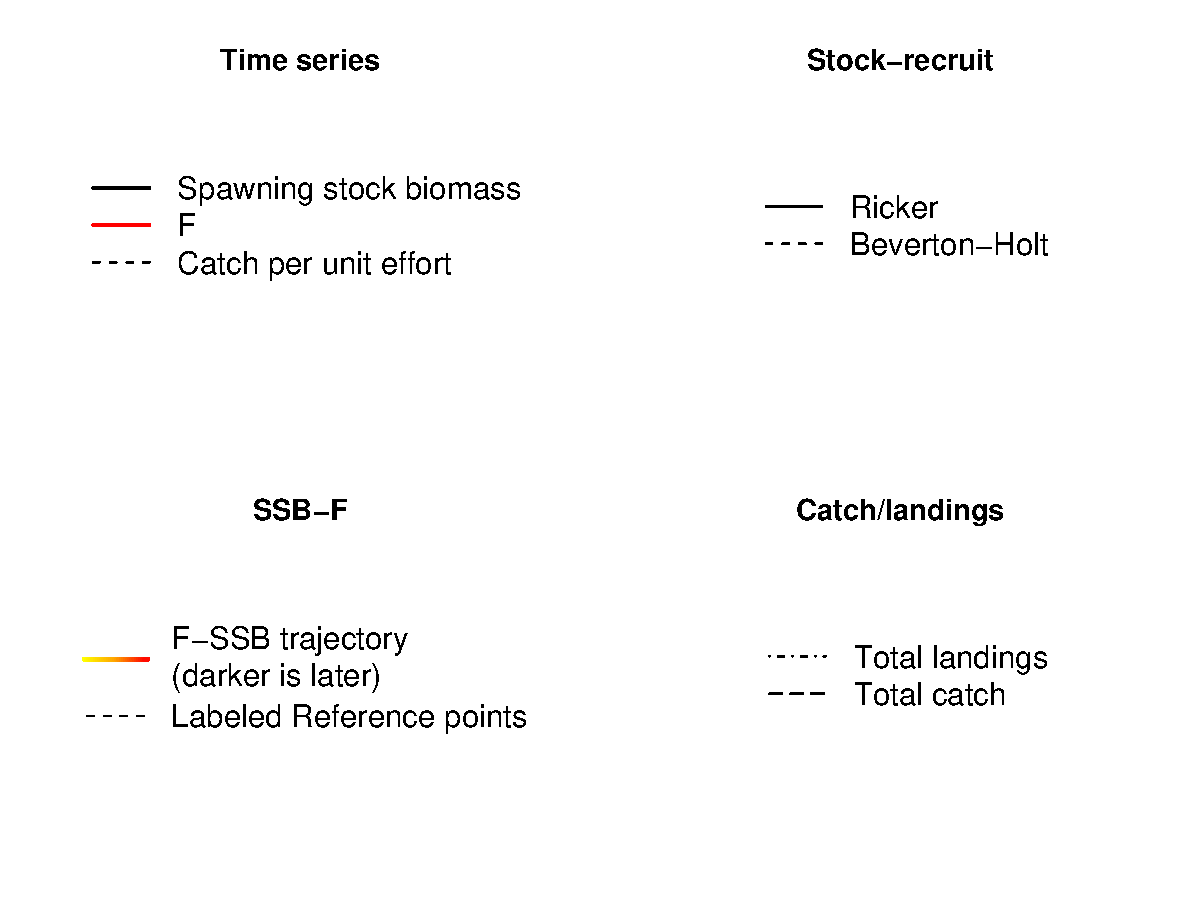
\includegraphics[width=1.2\textwidth]{../R/report_legend.pdf}
\caption{Line type specification for summary plots.}
\end{figure}

\end{center}


\section{Carcharhiniformes}\index{Carcharhiniformes}

\subsection{Carcharhinidae}\index{Carcharhinidae}\index{Carcharhiniformes!Carcharhinidae}

\subsubsection{Carcharhinus acronotus - Blacknose shark}\index{Blacknose shark}\index{Carcharhinus acronotus}\index{Carcharhinidae!Carcharhinus acronotus}
\begin{center}
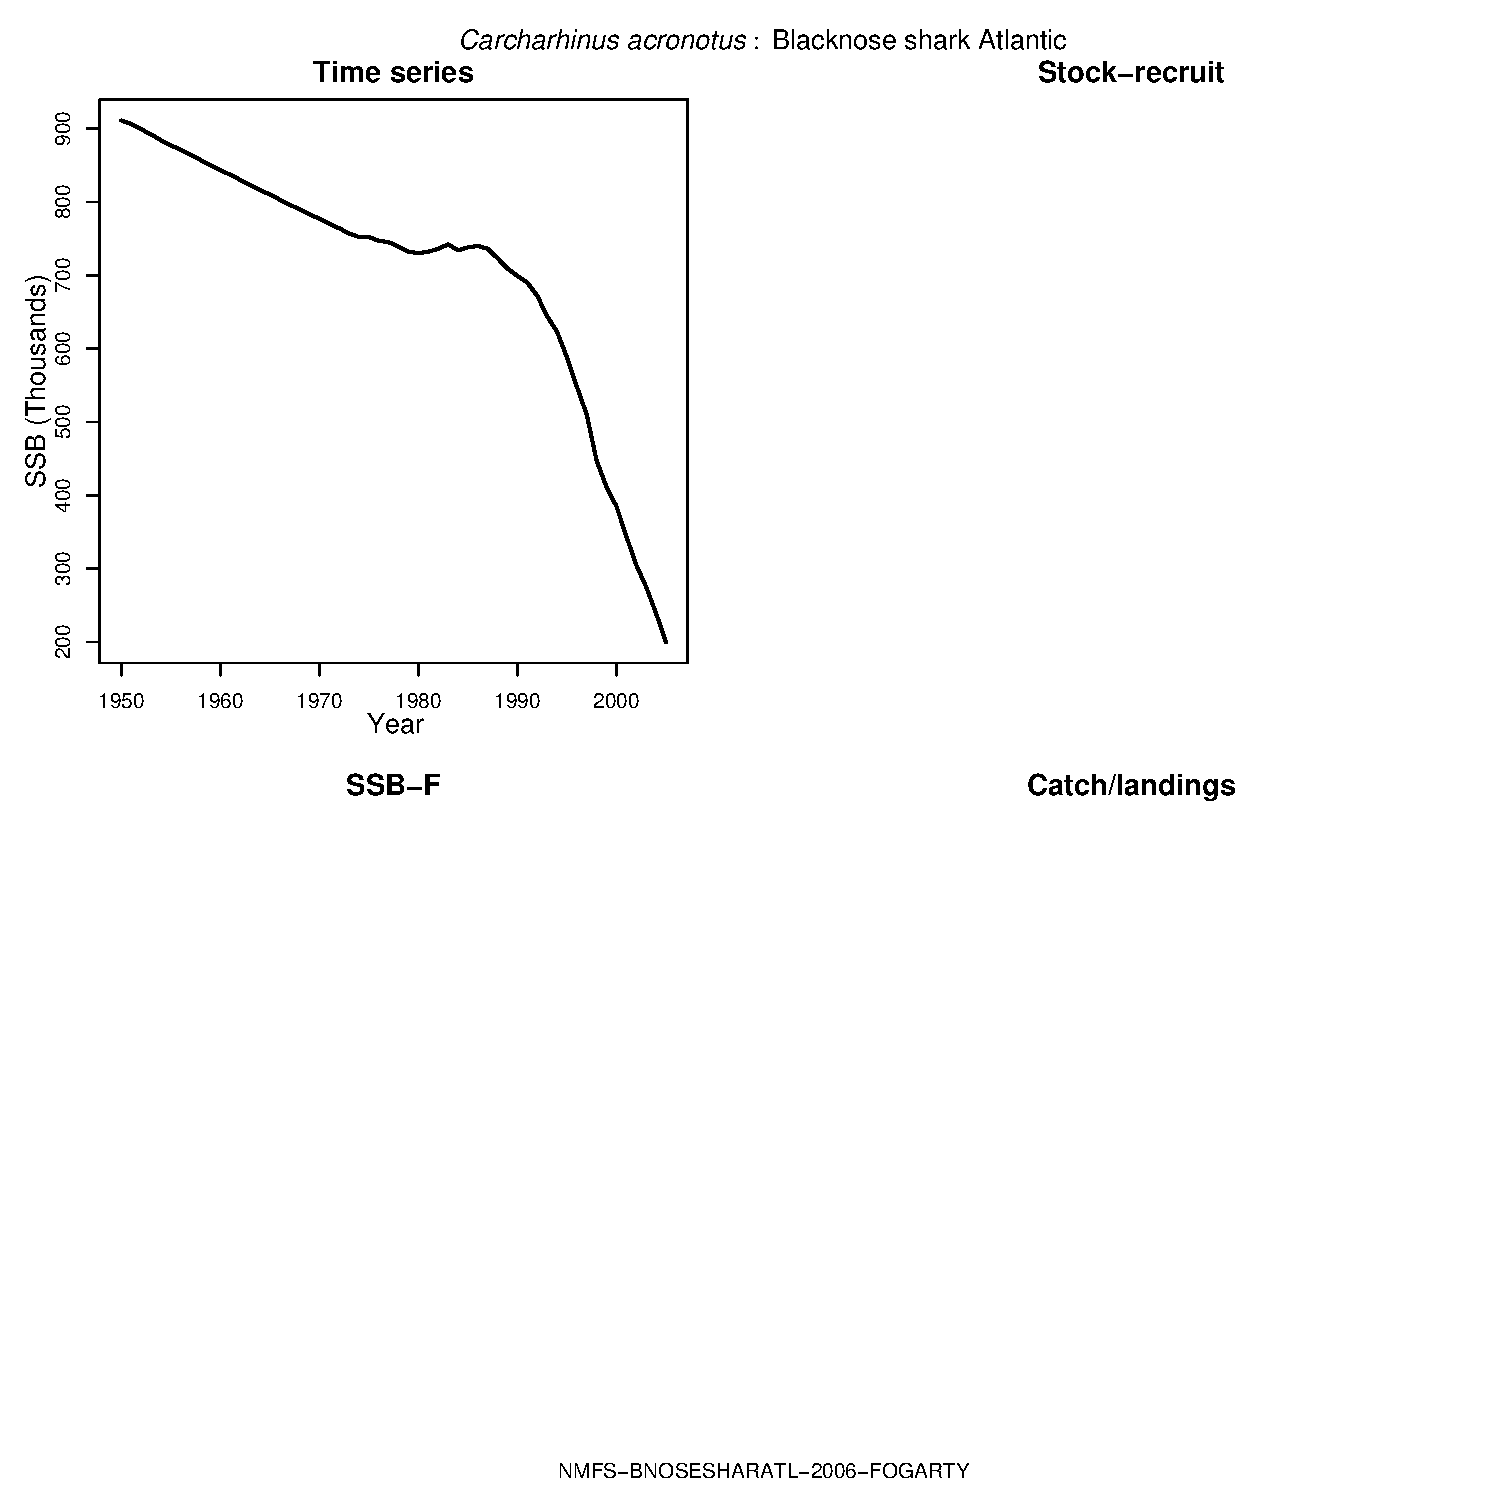
\includegraphics[width=1.2\textwidth]{../R/figures/NMFS-BNOSESHARATL-2006-FOGARTY.pdf}
\end{center}

\subsubsection{Carcharhinus limbatus - Blacktip shark}\index{Blacktip shark}\index{Carcharhinus limbatus}\index{Carcharhinidae!Carcharhinus limbatus}
\begin{center}
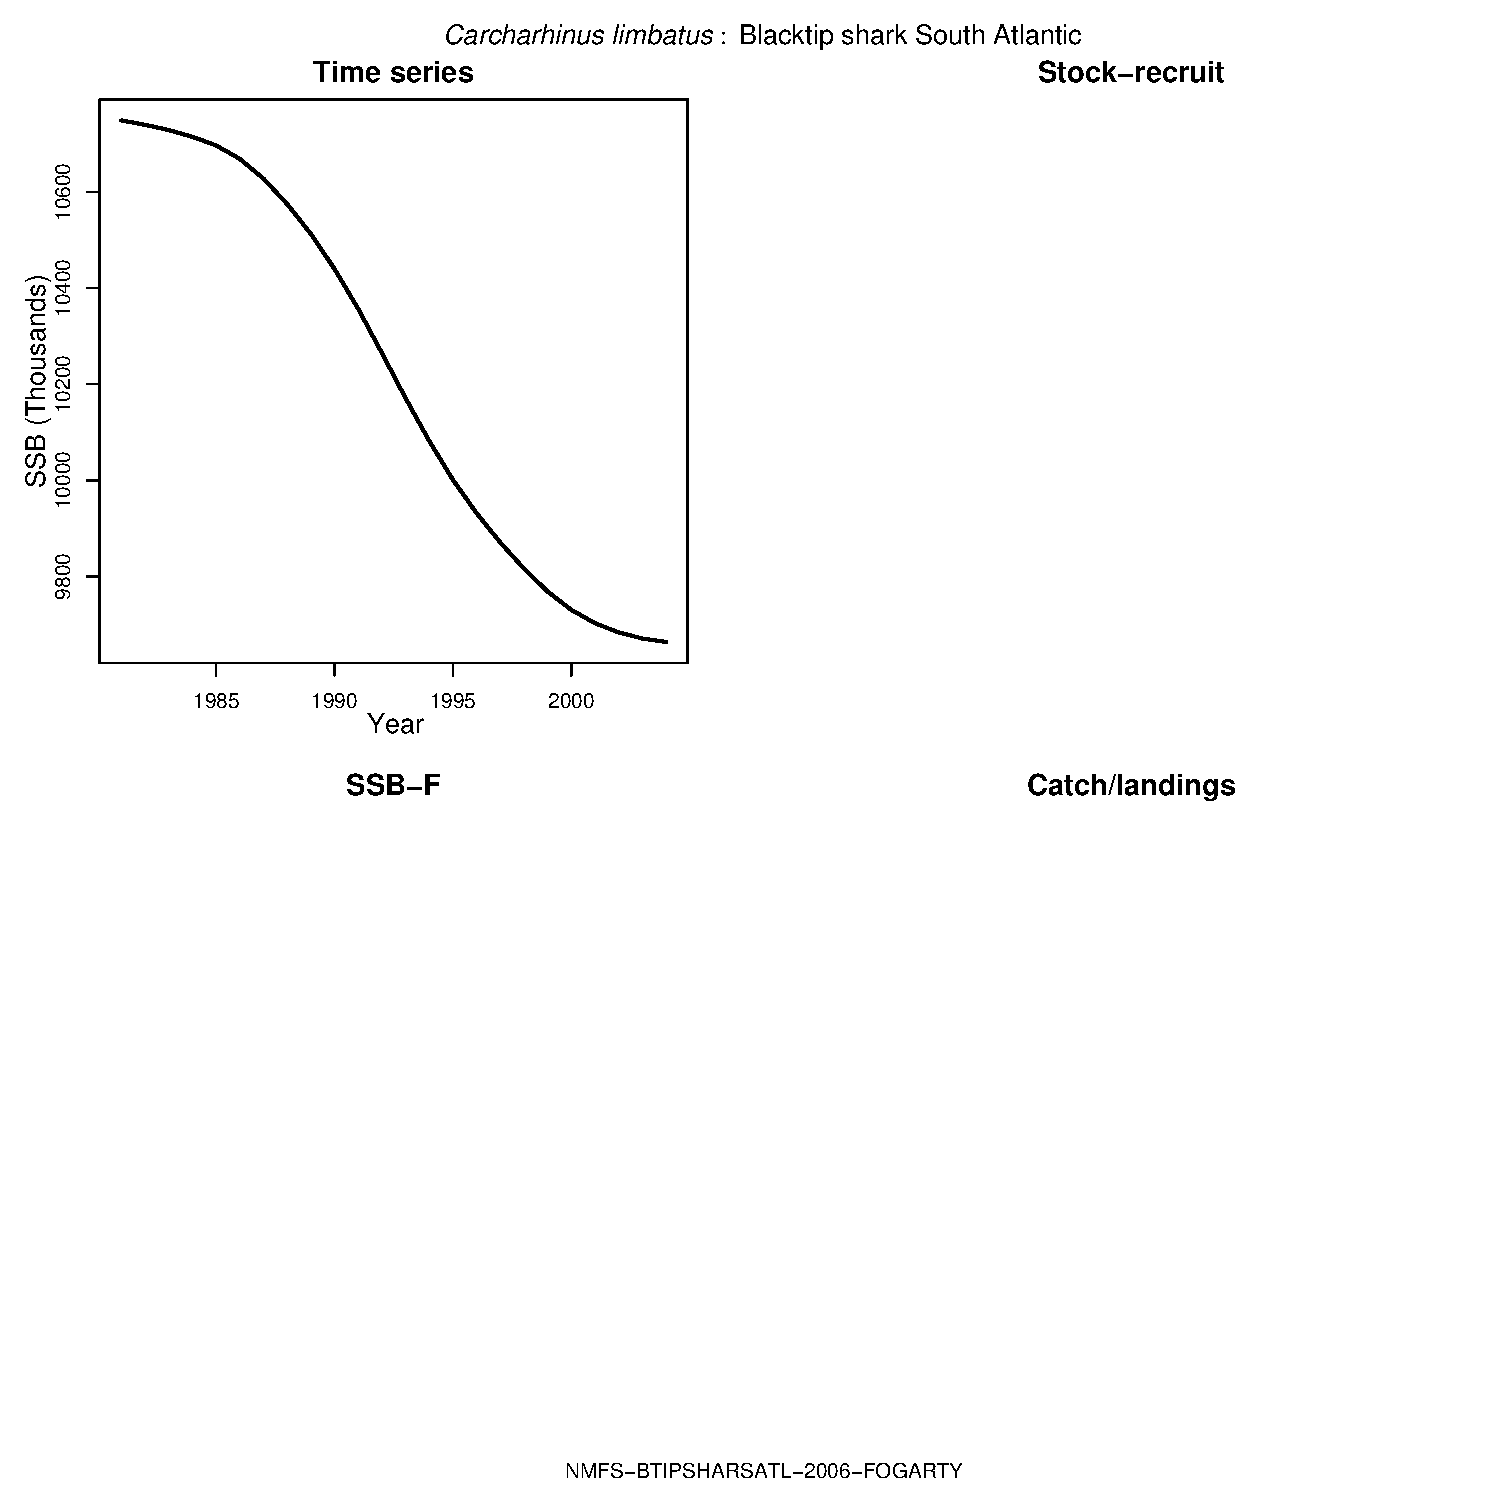
\includegraphics[width=1.2\textwidth]{../R/figures/NMFS-BTIPSHARSATL-2006-FOGARTY.pdf}
\end{center}

\subsubsection{Carcharhinus plumbeus - Sandbar shark}\index{Sandbar shark}\index{Carcharhinus plumbeus}\index{Carcharhinidae!Carcharhinus plumbeus}
\begin{center}
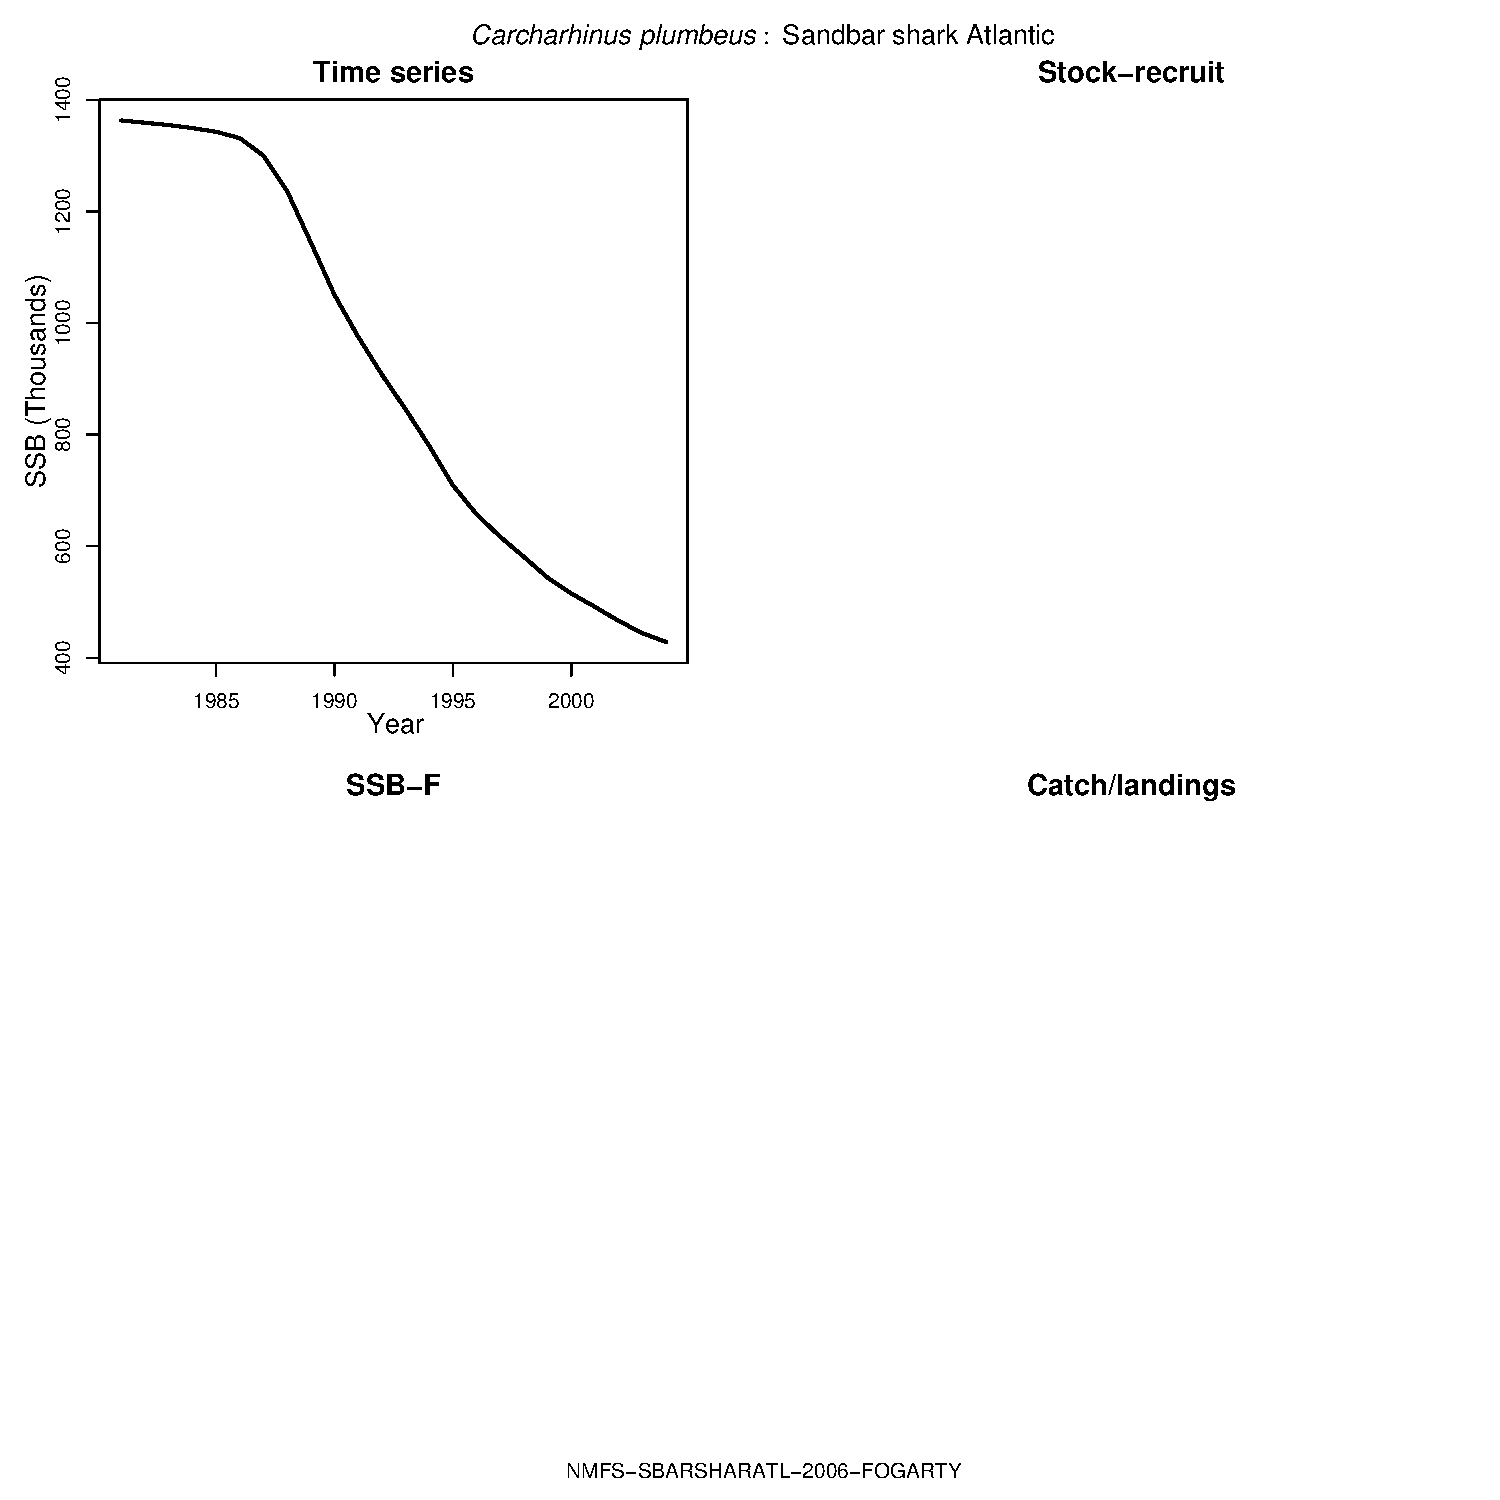
\includegraphics[width=1.2\textwidth]{../R/figures/NMFS-SBARSHARATL-2006-FOGARTY.pdf}
\end{center}

\subsubsection{Rhizoprionodon terraenovae - Atlantic sharpnose shark}\index{Atlantic sharpnose shark}\index{Rhizoprionodon terraenovae}\index{Carcharhinidae!Rhizoprionodon terraenovae}
\begin{center}
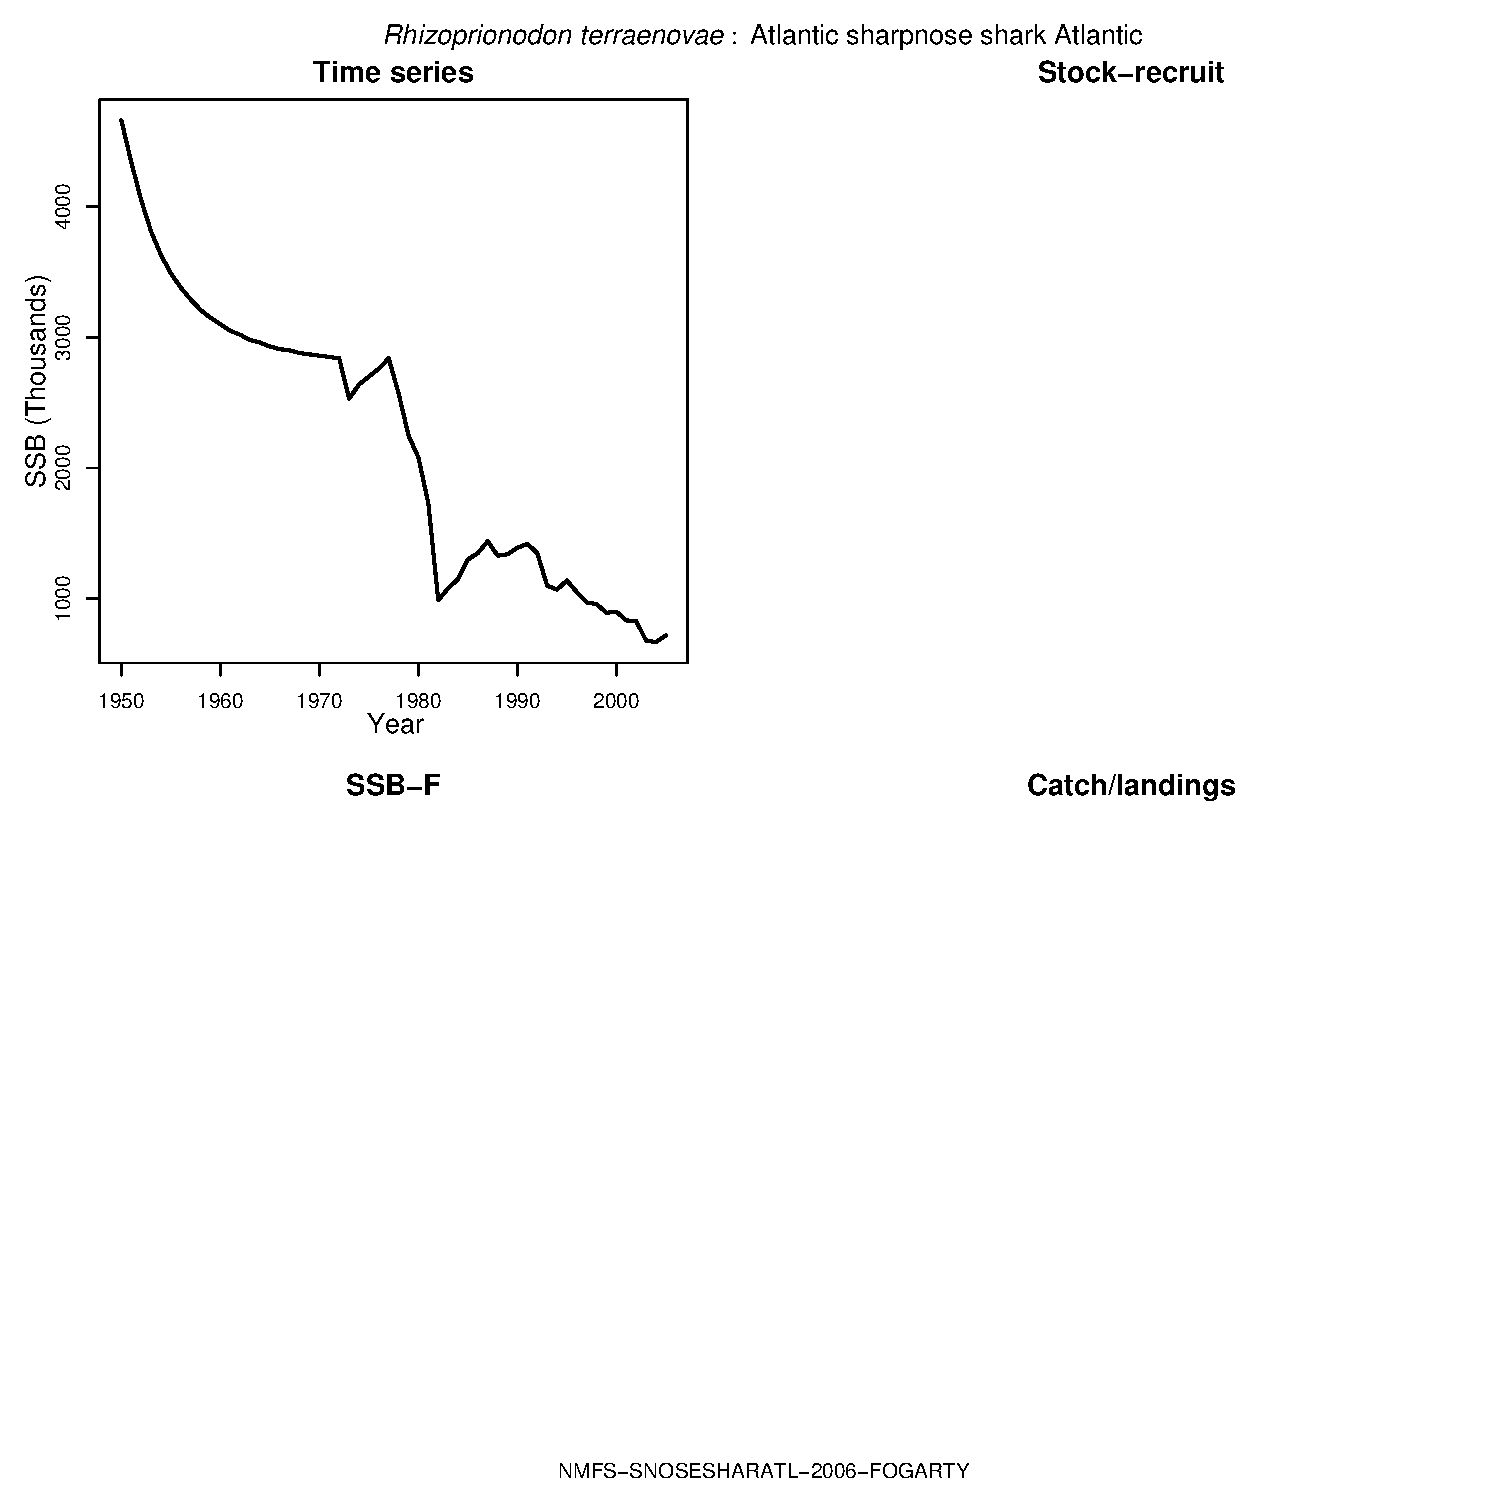
\includegraphics[width=1.2\textwidth]{../R/figures/NMFS-SNOSESHARATL-2006-FOGARTY.pdf}
\end{center}

\subsection{Sphyrnidae}\index{Sphyrnidae}\index{Carcharhiniformes!Sphyrnidae}

\subsubsection{Sphyrna tiburo - Bonnethead shark}\index{Bonnethead shark}\index{Sphyrna tiburo}\index{Sphyrnidae!Sphyrna tiburo}
\begin{center}
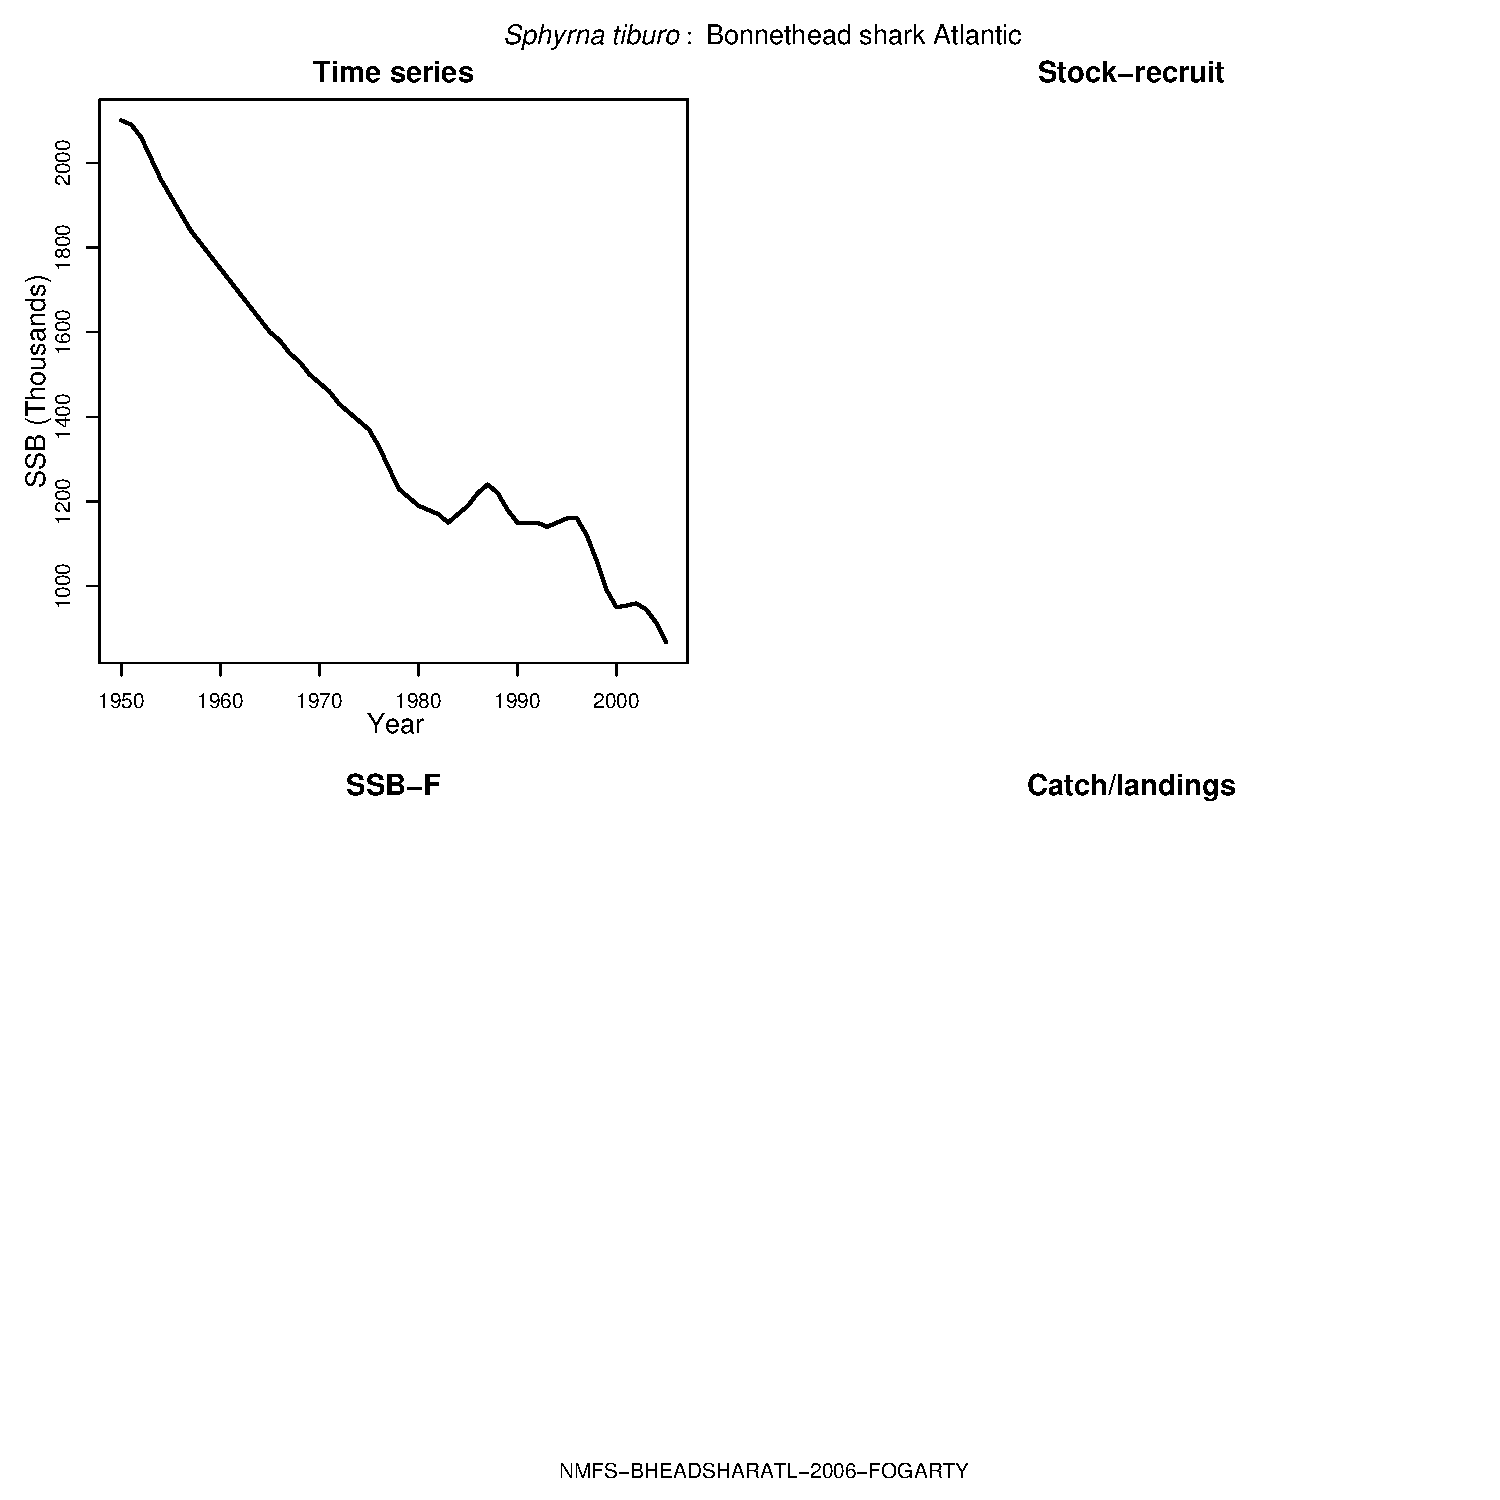
\includegraphics[width=1.2\textwidth]{../R/figures/NMFS-BHEADSHARATL-2006-FOGARTY.pdf}
\end{center}

\section{Clupeiformes}\index{Clupeiformes}

\subsection{Clupeidae}\index{Clupeidae}\index{Clupeiformes!Clupeidae}

\subsubsection{Clupea harengus - Herring}\index{Herring}\index{Clupea harengus}\index{Clupeidae!Clupea harengus}
\begin{center}
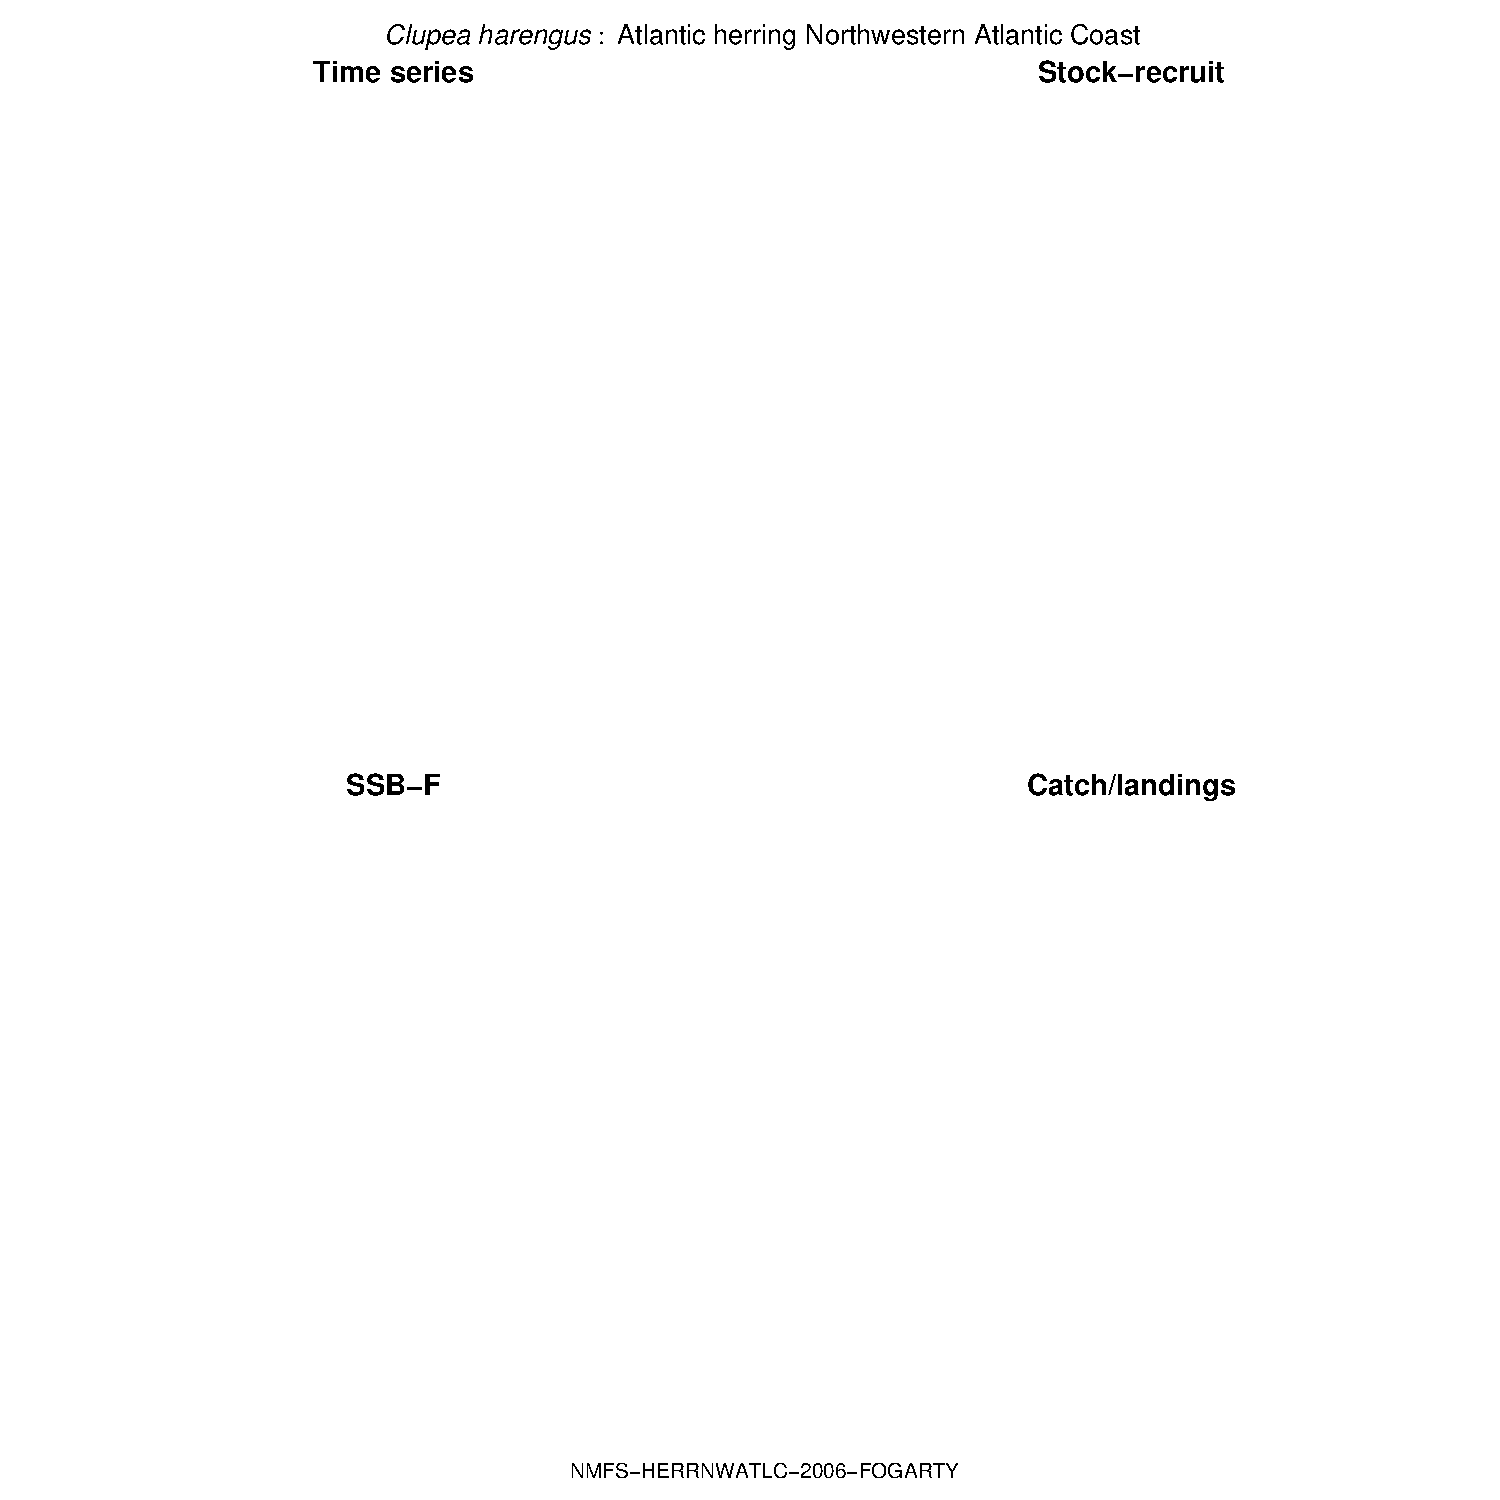
\includegraphics[width=1.2\textwidth]{../R/figures/NMFS-HERRNWATLC-2006-FOGARTY.pdf}
\end{center}

\subsubsection{Clupea harengus - Herring}\index{Herring}\index{Clupea harengus}\index{Clupeidae!Clupea harengus}
\begin{center}
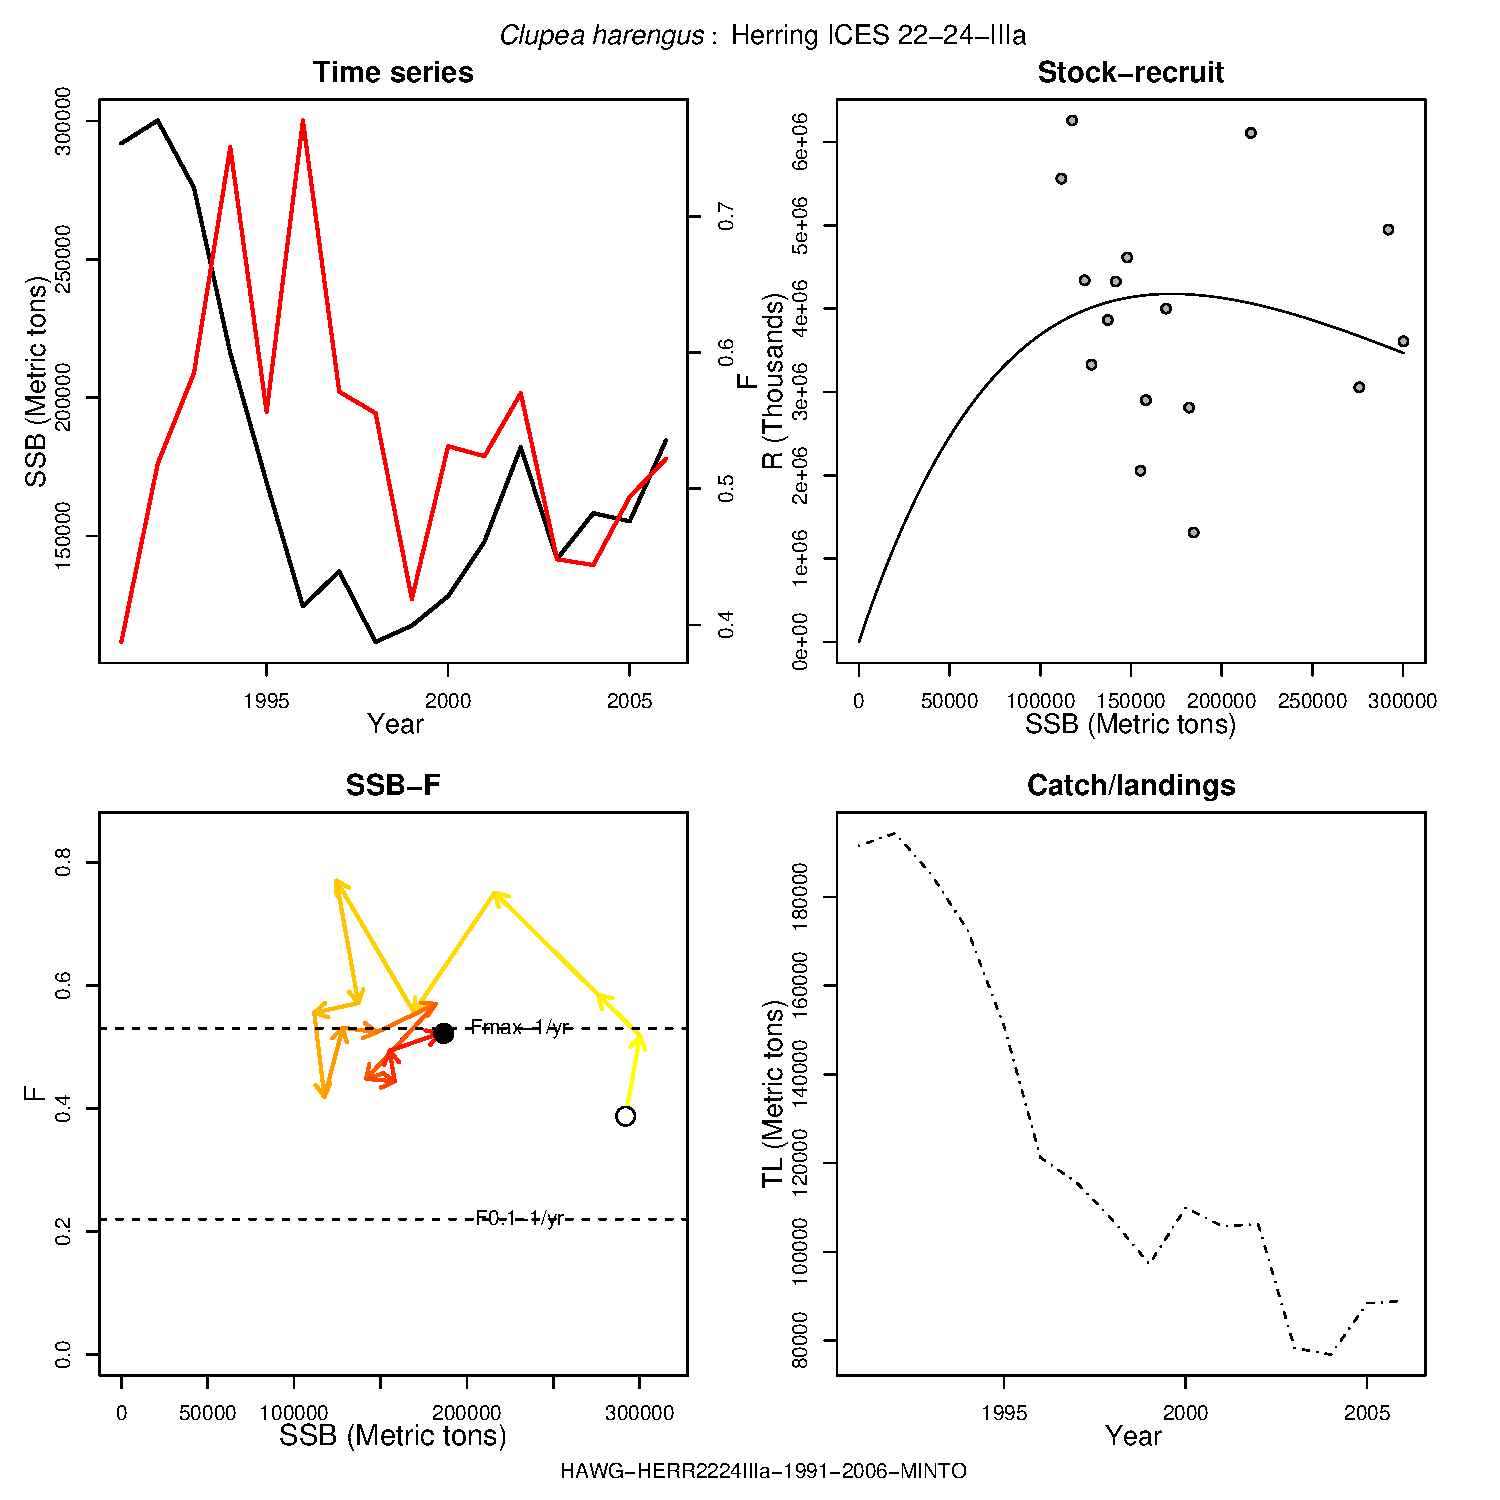
\includegraphics[width=1.2\textwidth]{../R/figures/HAWG-HERR2224IIIa-1991-2006-MINTO.pdf}
\end{center}

\subsubsection{Clupea harengus - Herring}\index{Herring}\index{Clupea harengus}\index{Clupeidae!Clupea harengus}
\begin{center}
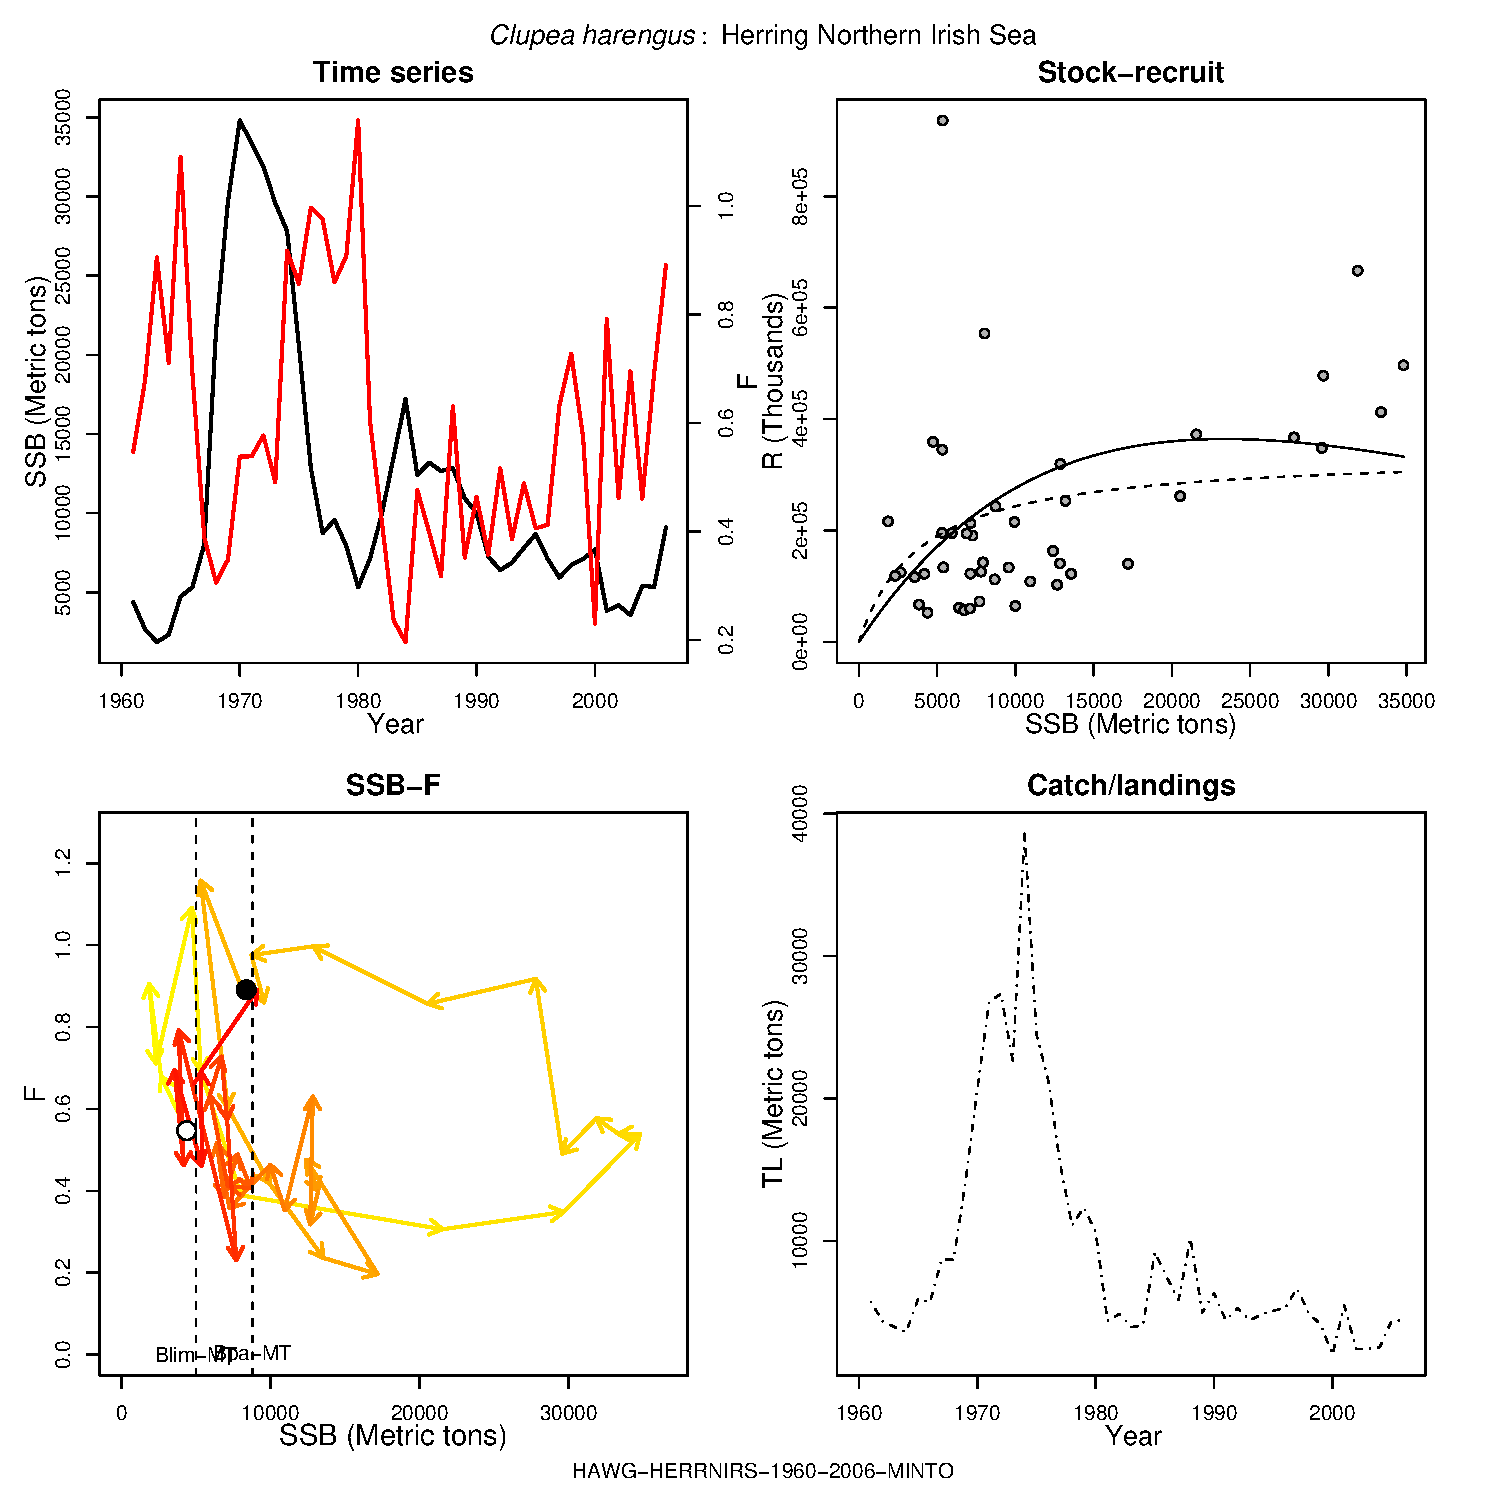
\includegraphics[width=1.2\textwidth]{../R/figures/HAWG-HERRNIRS-1960-2006-MINTO.pdf}
\end{center}

\subsubsection{Clupea harengus - Herring}\index{Herring}\index{Clupea harengus}\index{Clupeidae!Clupea harengus}
\begin{center}
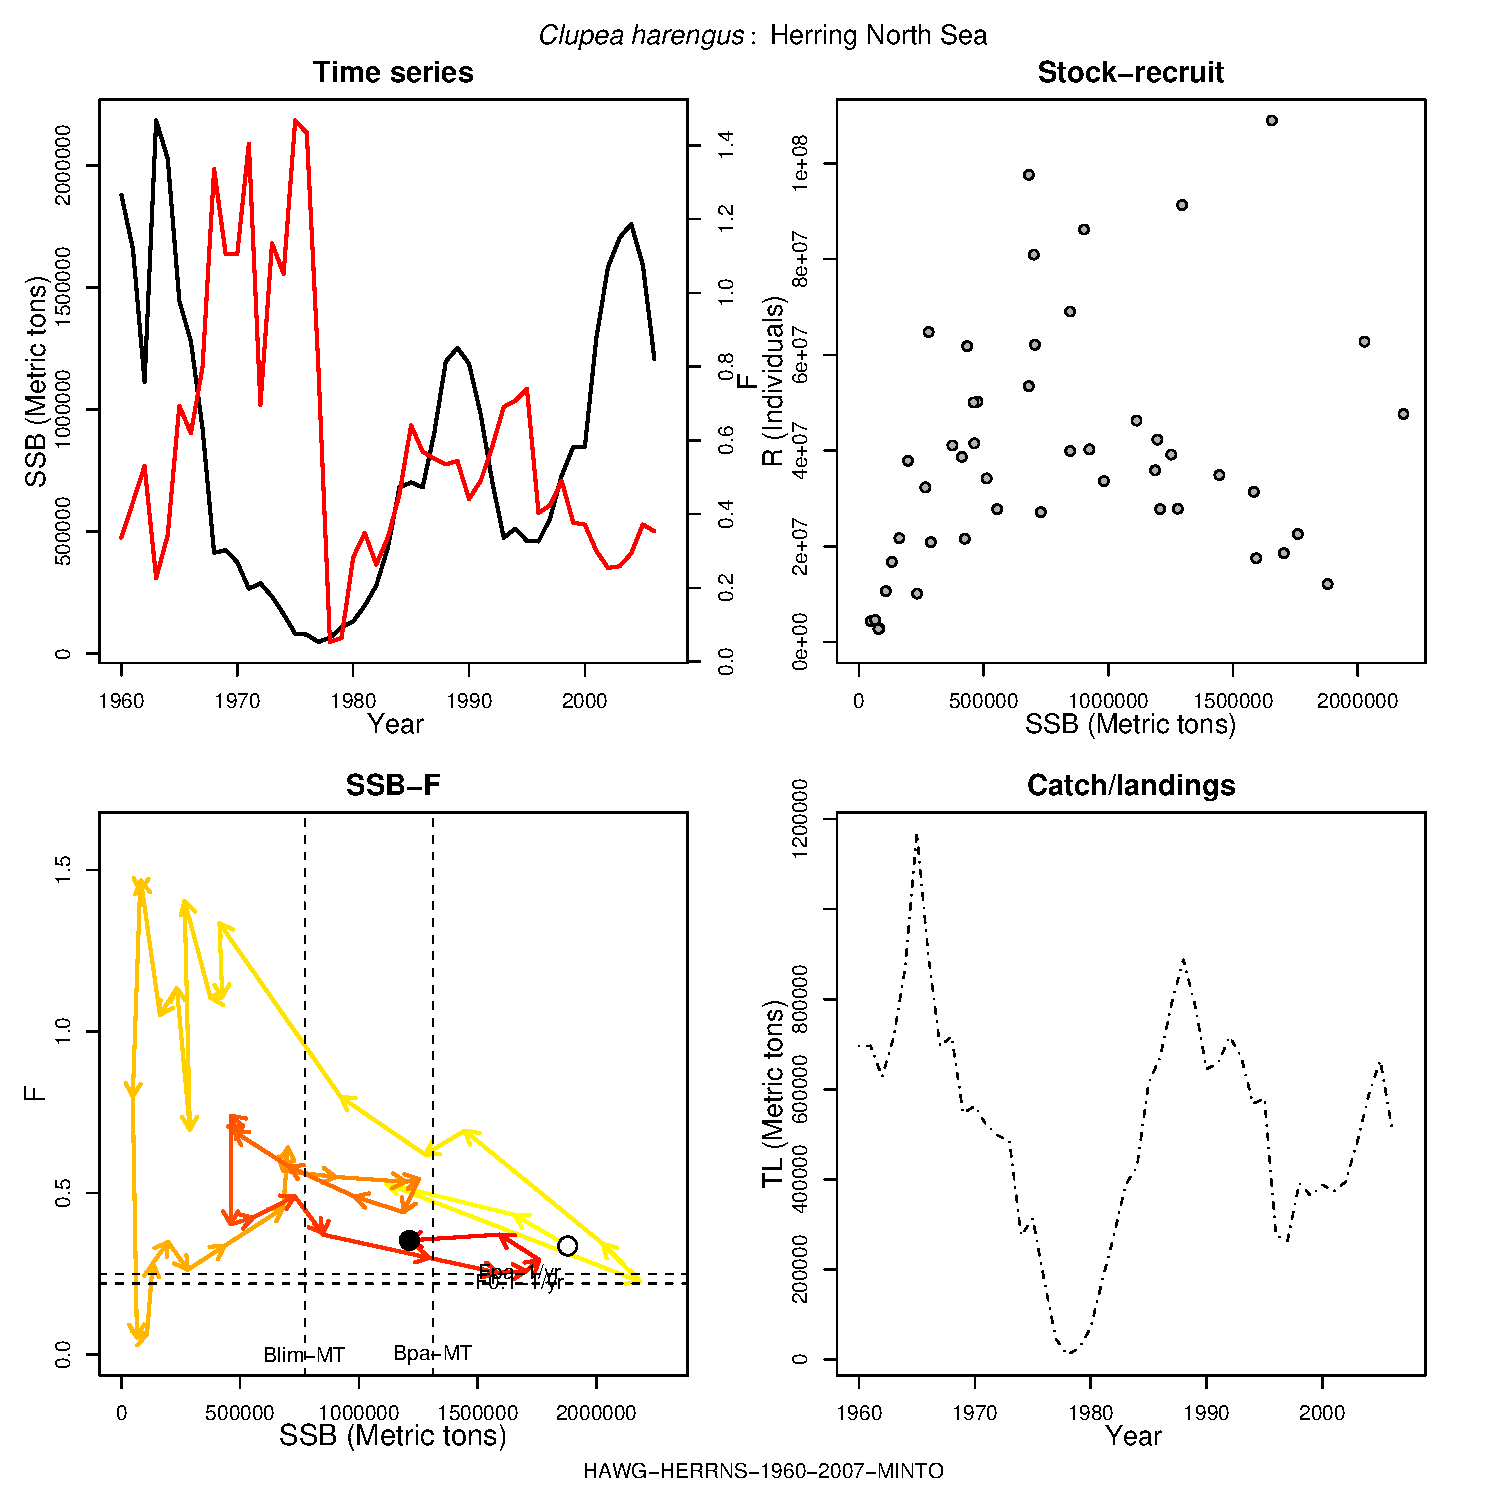
\includegraphics[width=1.2\textwidth]{../R/figures/HAWG-HERRNS-1960-2007-MINTO.pdf}
\end{center}

\subsubsection{Clupea harengus - Herring}\index{Herring}\index{Clupea harengus}\index{Clupeidae!Clupea harengus}
\begin{center}
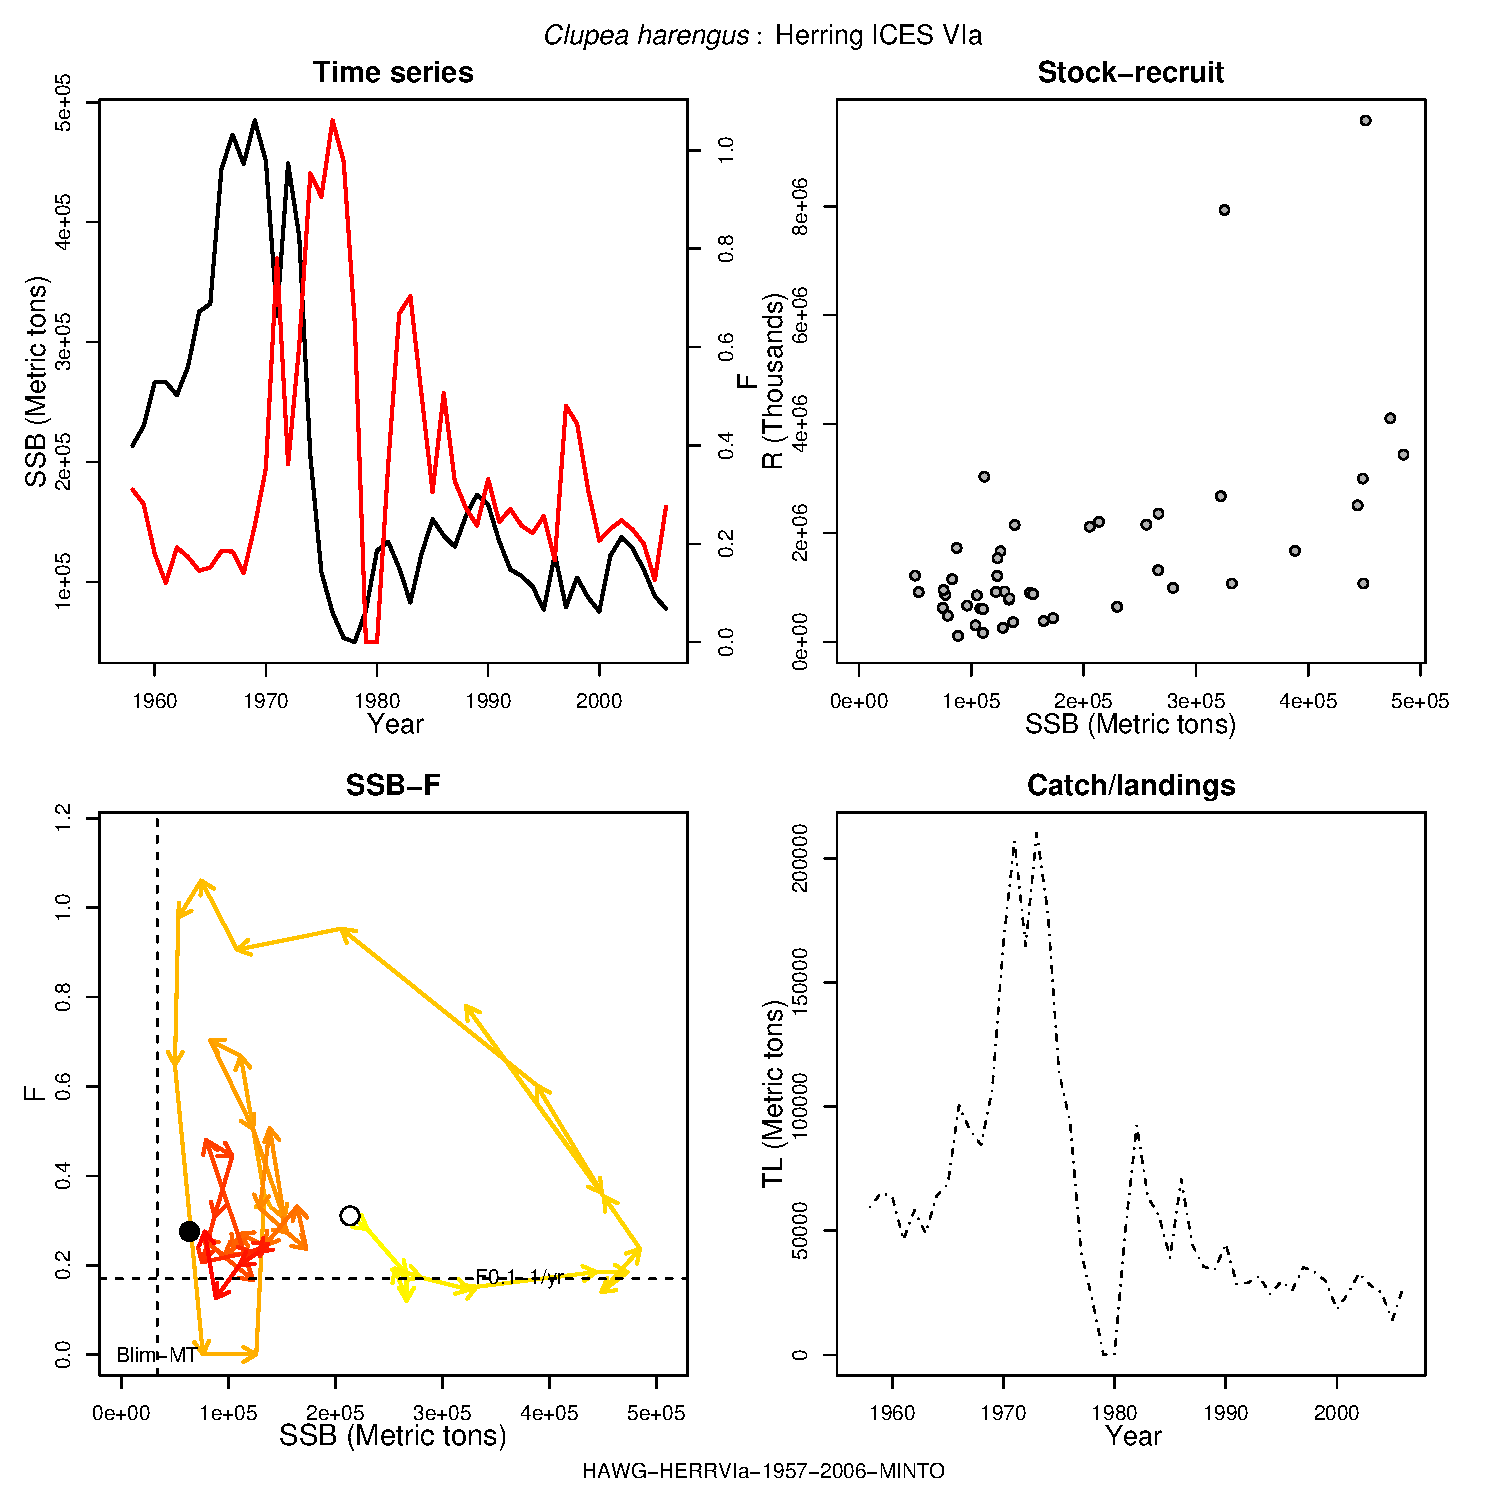
\includegraphics[width=1.2\textwidth]{../R/figures/HAWG-HERRVIa-1957-2006-MINTO.pdf}
\end{center}

\subsubsection{Clupea harengus - Herring}\index{Herring}\index{Clupea harengus}\index{Clupeidae!Clupea harengus}
\begin{center}
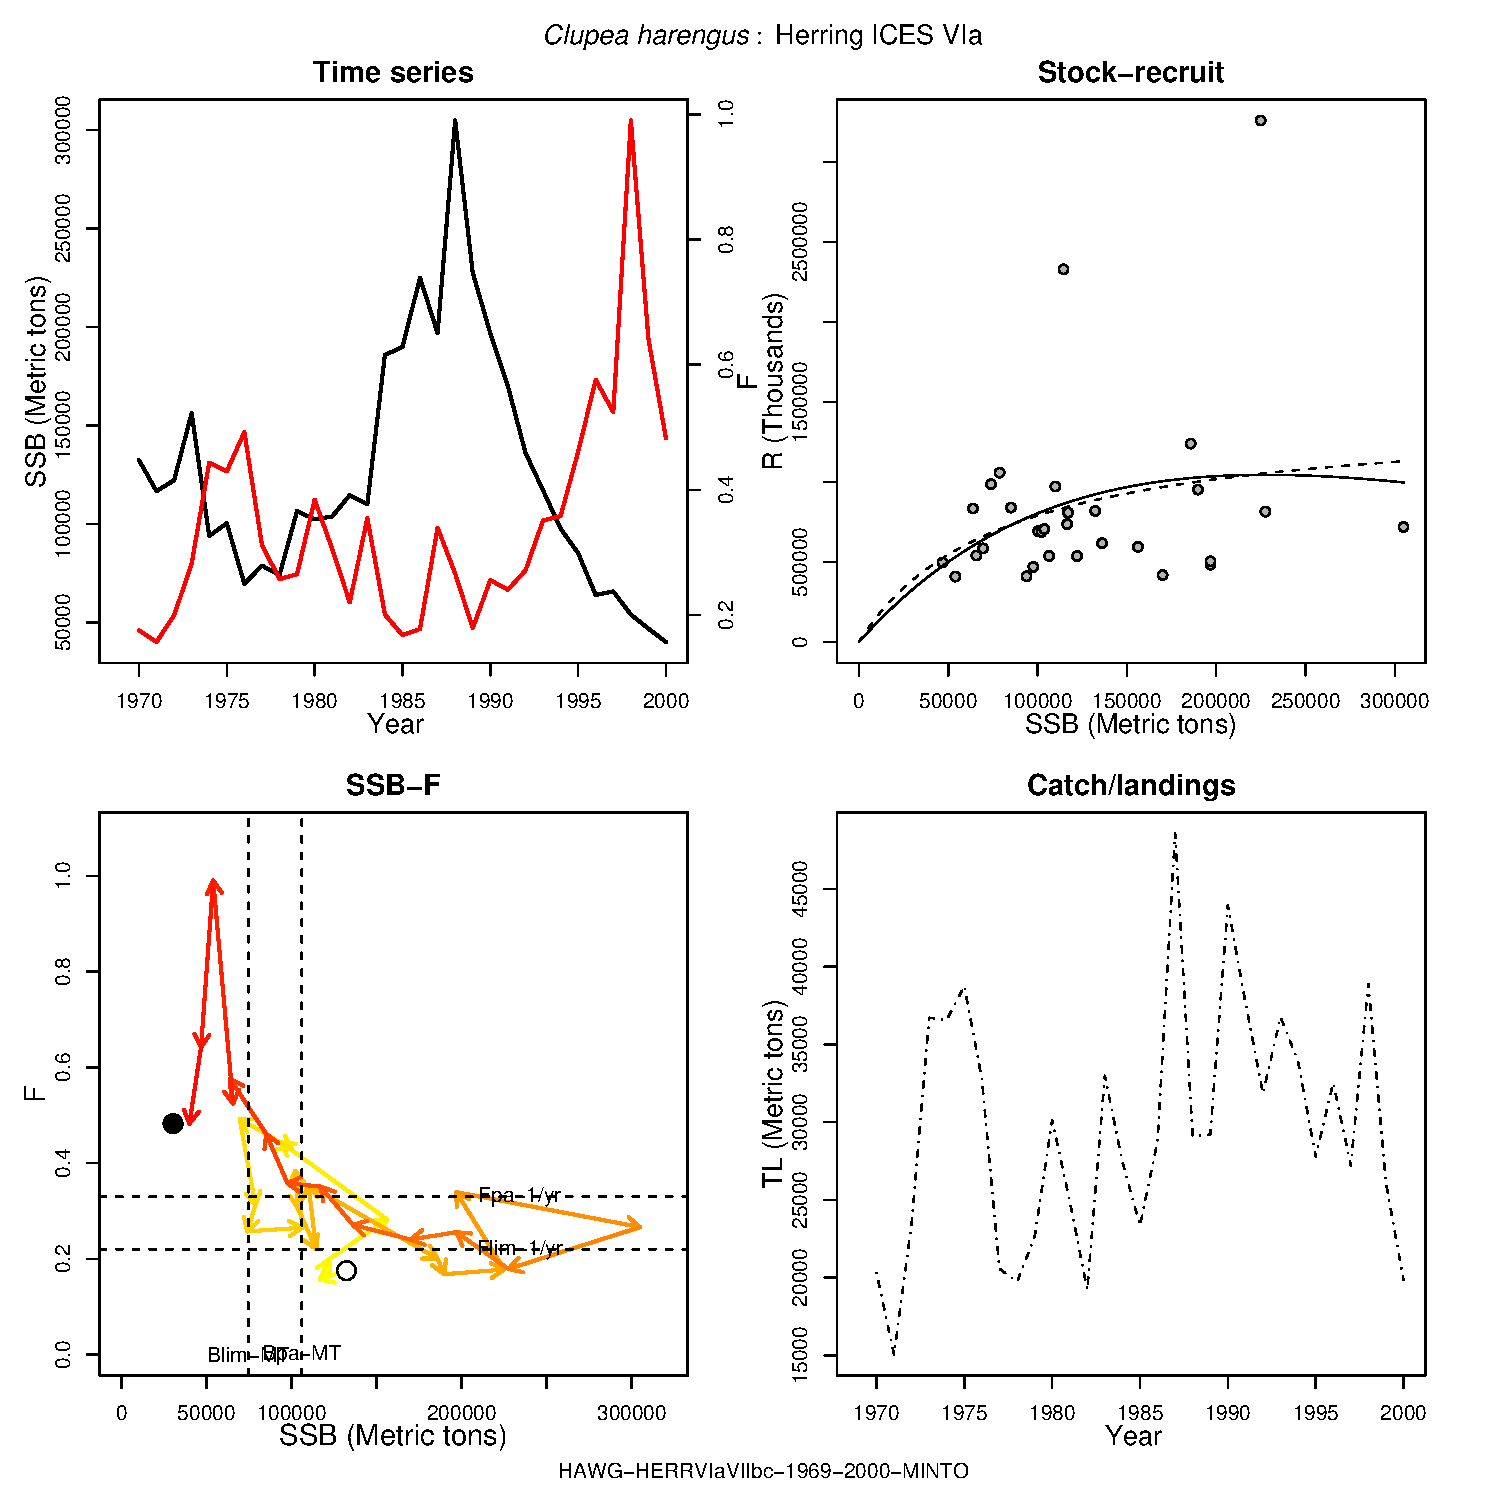
\includegraphics[width=1.2\textwidth]{../R/figures/HAWG-HERRVIaVIIbc-1969-2000-MINTO.pdf}
\end{center}

\subsubsection{Clupea harengus - Herring}\index{Herring}\index{Clupea harengus}\index{Clupeidae!Clupea harengus}
\begin{center}
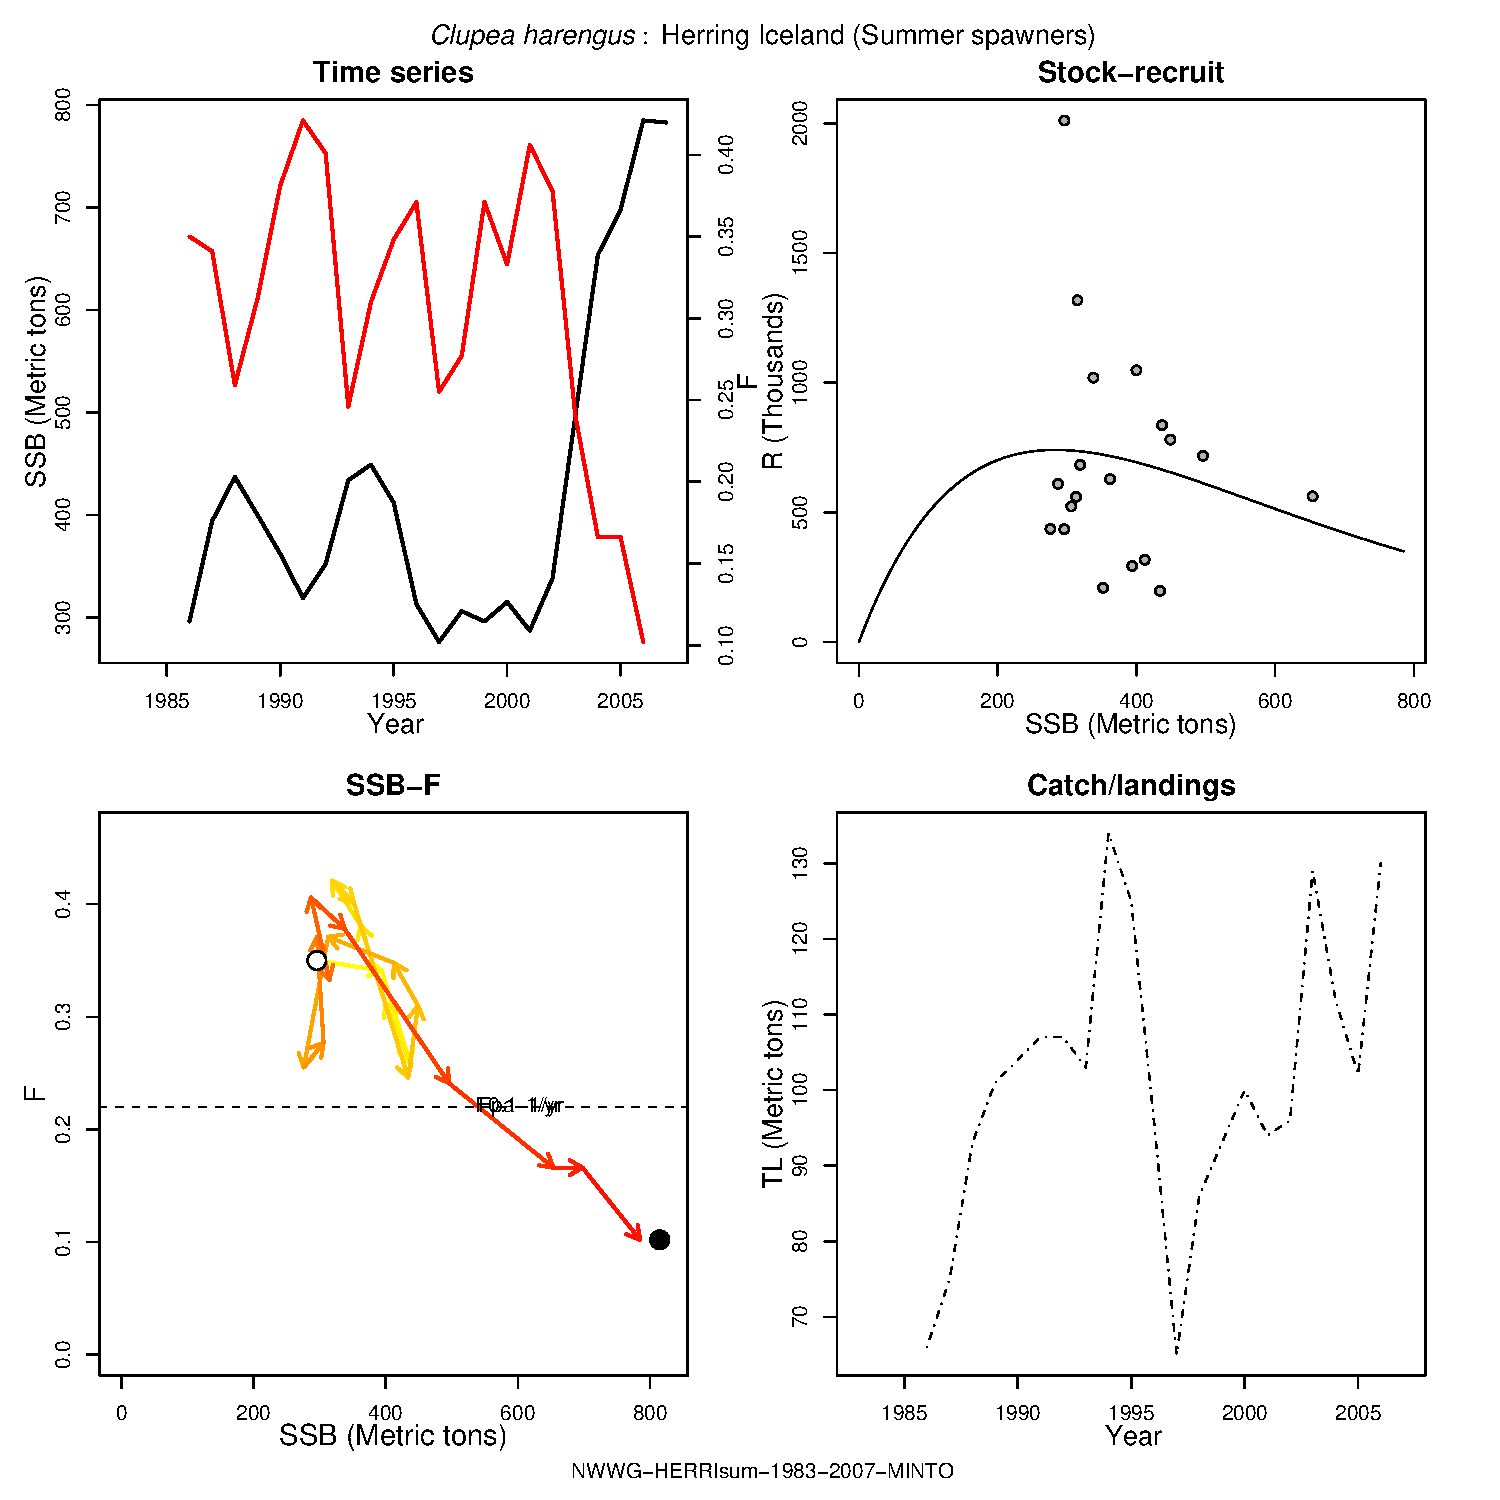
\includegraphics[width=1.2\textwidth]{../R/figures/NWWG-HERRIsum-1983-2007-MINTO.pdf}
\end{center}

\subsubsection{Clupea harengus - Herring}\index{Herring}\index{Clupea harengus}\index{Clupeidae!Clupea harengus}
\begin{center}
\includegraphics[width=1.2\textwidth]{../R/figures/PHONYassessorid-HERRIsum-1946-2000-MYERS.pdf}
\end{center}

\subsubsection{Clupea harengus - Herring}\index{Herring}\index{Clupea harengus}\index{Clupeidae!Clupea harengus}
\begin{center}
\includegraphics[width=1.2\textwidth]{../R/figures/PHONYassessorid-HERRNIRS-1971-2000-MYERS.pdf}
\end{center}

\subsubsection{Clupea harengus - Herring}\index{Herring}\index{Clupea harengus}\index{Clupeidae!Clupea harengus}
\begin{center}
\includegraphics[width=1.2\textwidth]{../R/figures/PHONYassessorid-HERRNS-1903-1990-MYERS.pdf}
\end{center}

\subsubsection{Clupea harengus - Herring}\index{Herring}\index{Clupea harengus}\index{Clupeidae!Clupea harengus}
\begin{center}
\includegraphics[width=1.2\textwidth]{../R/figures/PHONYassessorid-HERRVIaVIIbc-1969-2000-MYERS.pdf}
\end{center}

\subsubsection{Clupea harengus - Herring}\index{Herring}\index{Clupea harengus}\index{Clupeidae!Clupea harengus}
\begin{center}
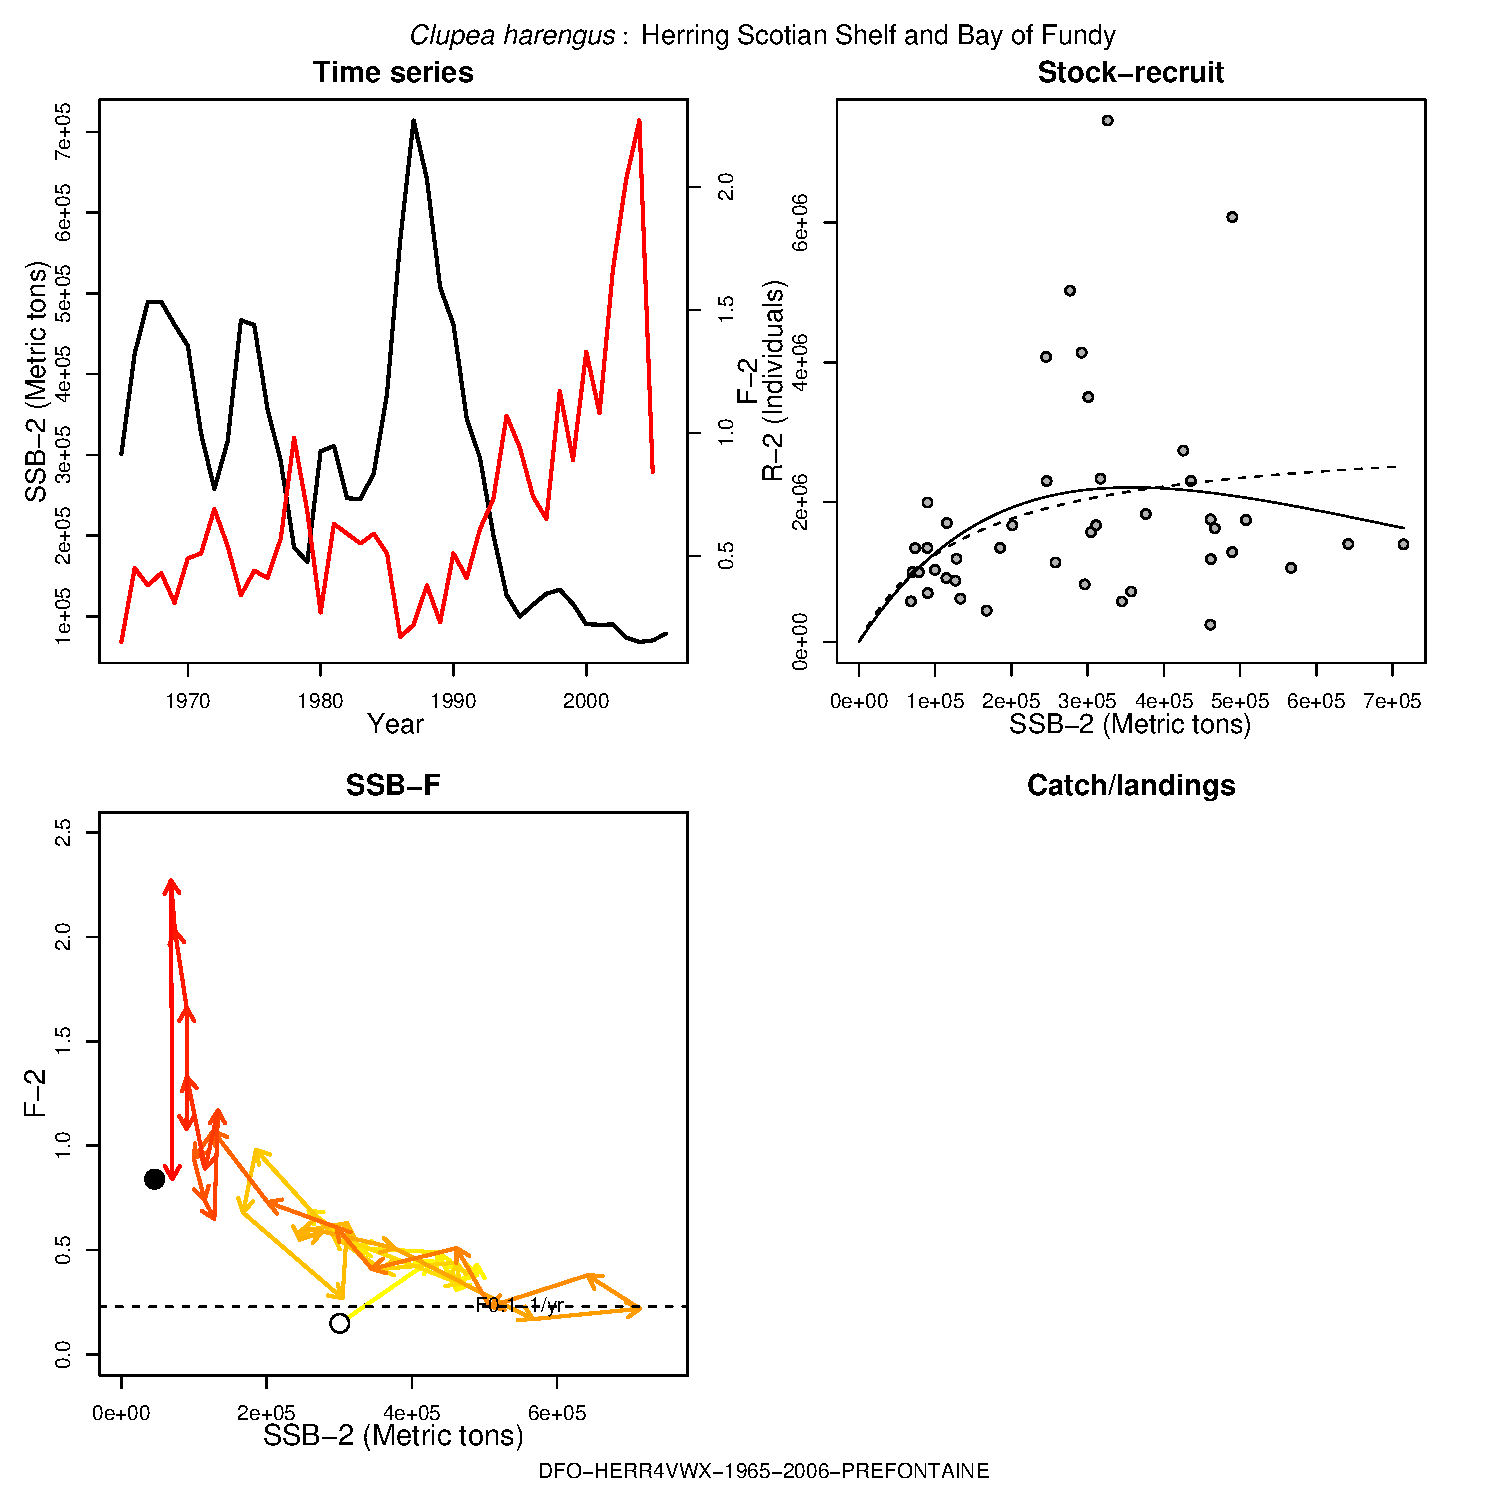
\includegraphics[width=1.2\textwidth]{../R/figures/DFO-HERR4VWX-1965-2006-PREFONTAINE.pdf}
\end{center}

\subsubsection{Clupea harengus - Herring}\index{Herring}\index{Clupea harengus}\index{Clupeidae!Clupea harengus}
\begin{center}
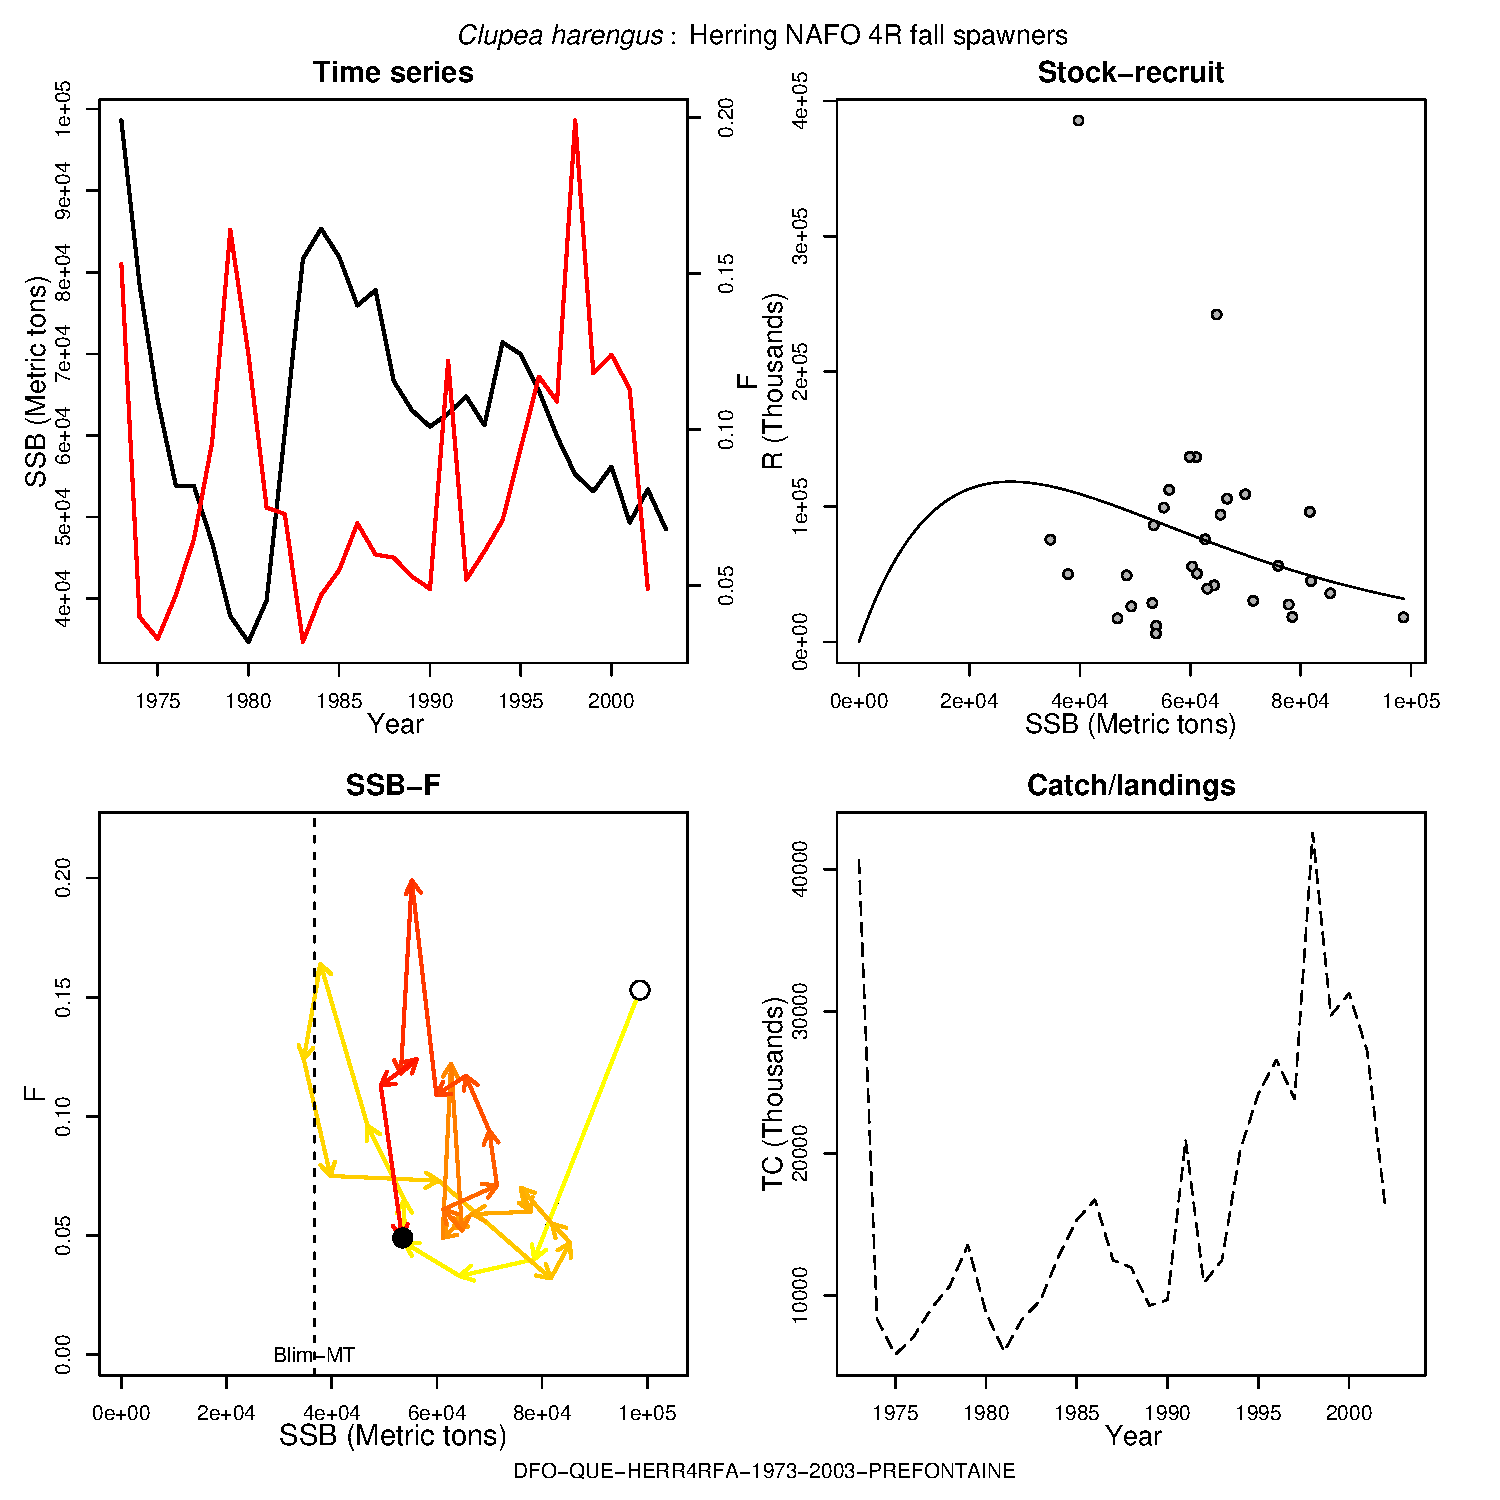
\includegraphics[width=1.2\textwidth]{../R/figures/DFO-QUE-HERR4RFA-1973-2003-PREFONTAINE.pdf}
\end{center}

\subsubsection{Clupea harengus - Herring}\index{Herring}\index{Clupea harengus}\index{Clupeidae!Clupea harengus}
\begin{center}
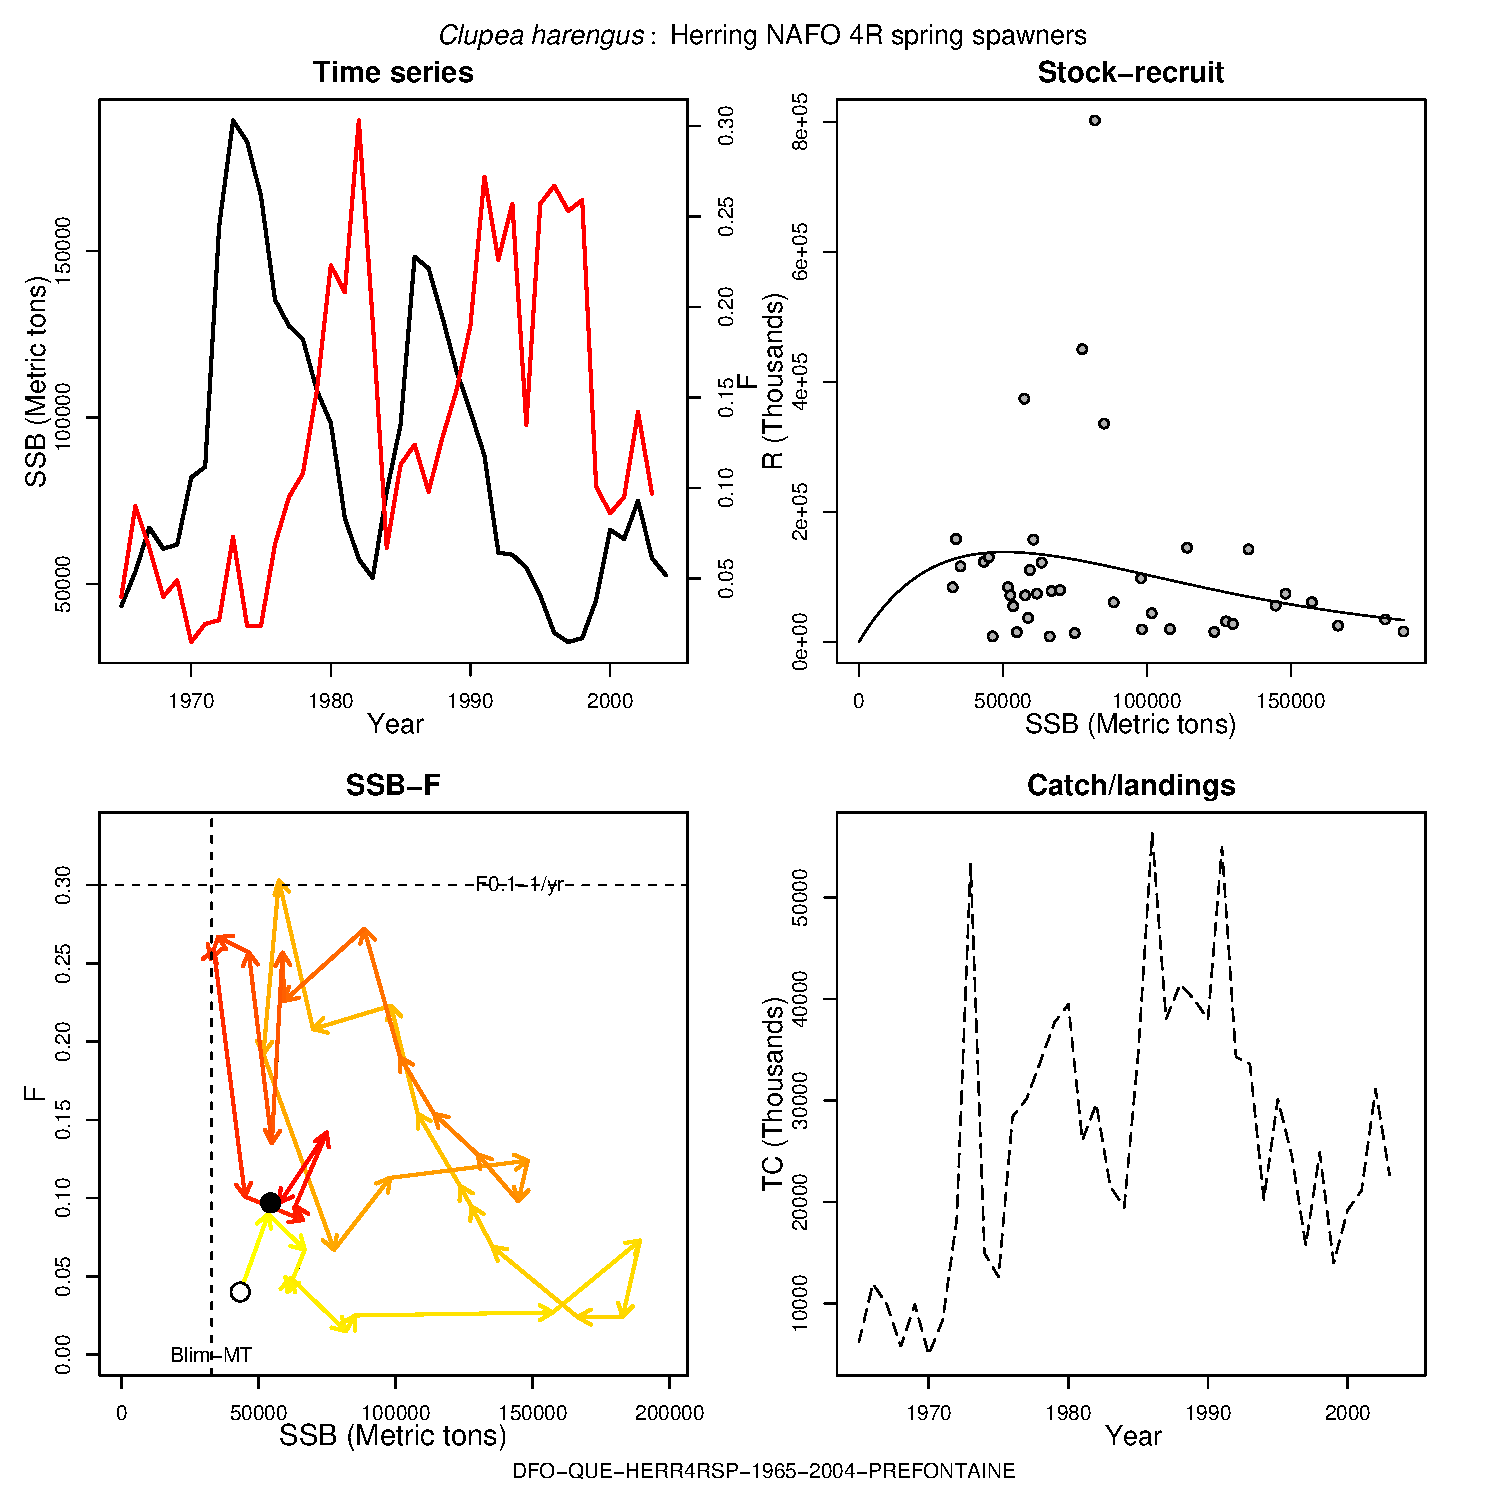
\includegraphics[width=1.2\textwidth]{../R/figures/DFO-QUE-HERR4RSP-1965-2004-PREFONTAINE.pdf}
\end{center}

\subsubsection{Clupea pallasii - Pacific herring}\index{Pacific herring}\index{Clupea pallasii}\index{Clupeidae!Clupea pallasii}
\begin{center}
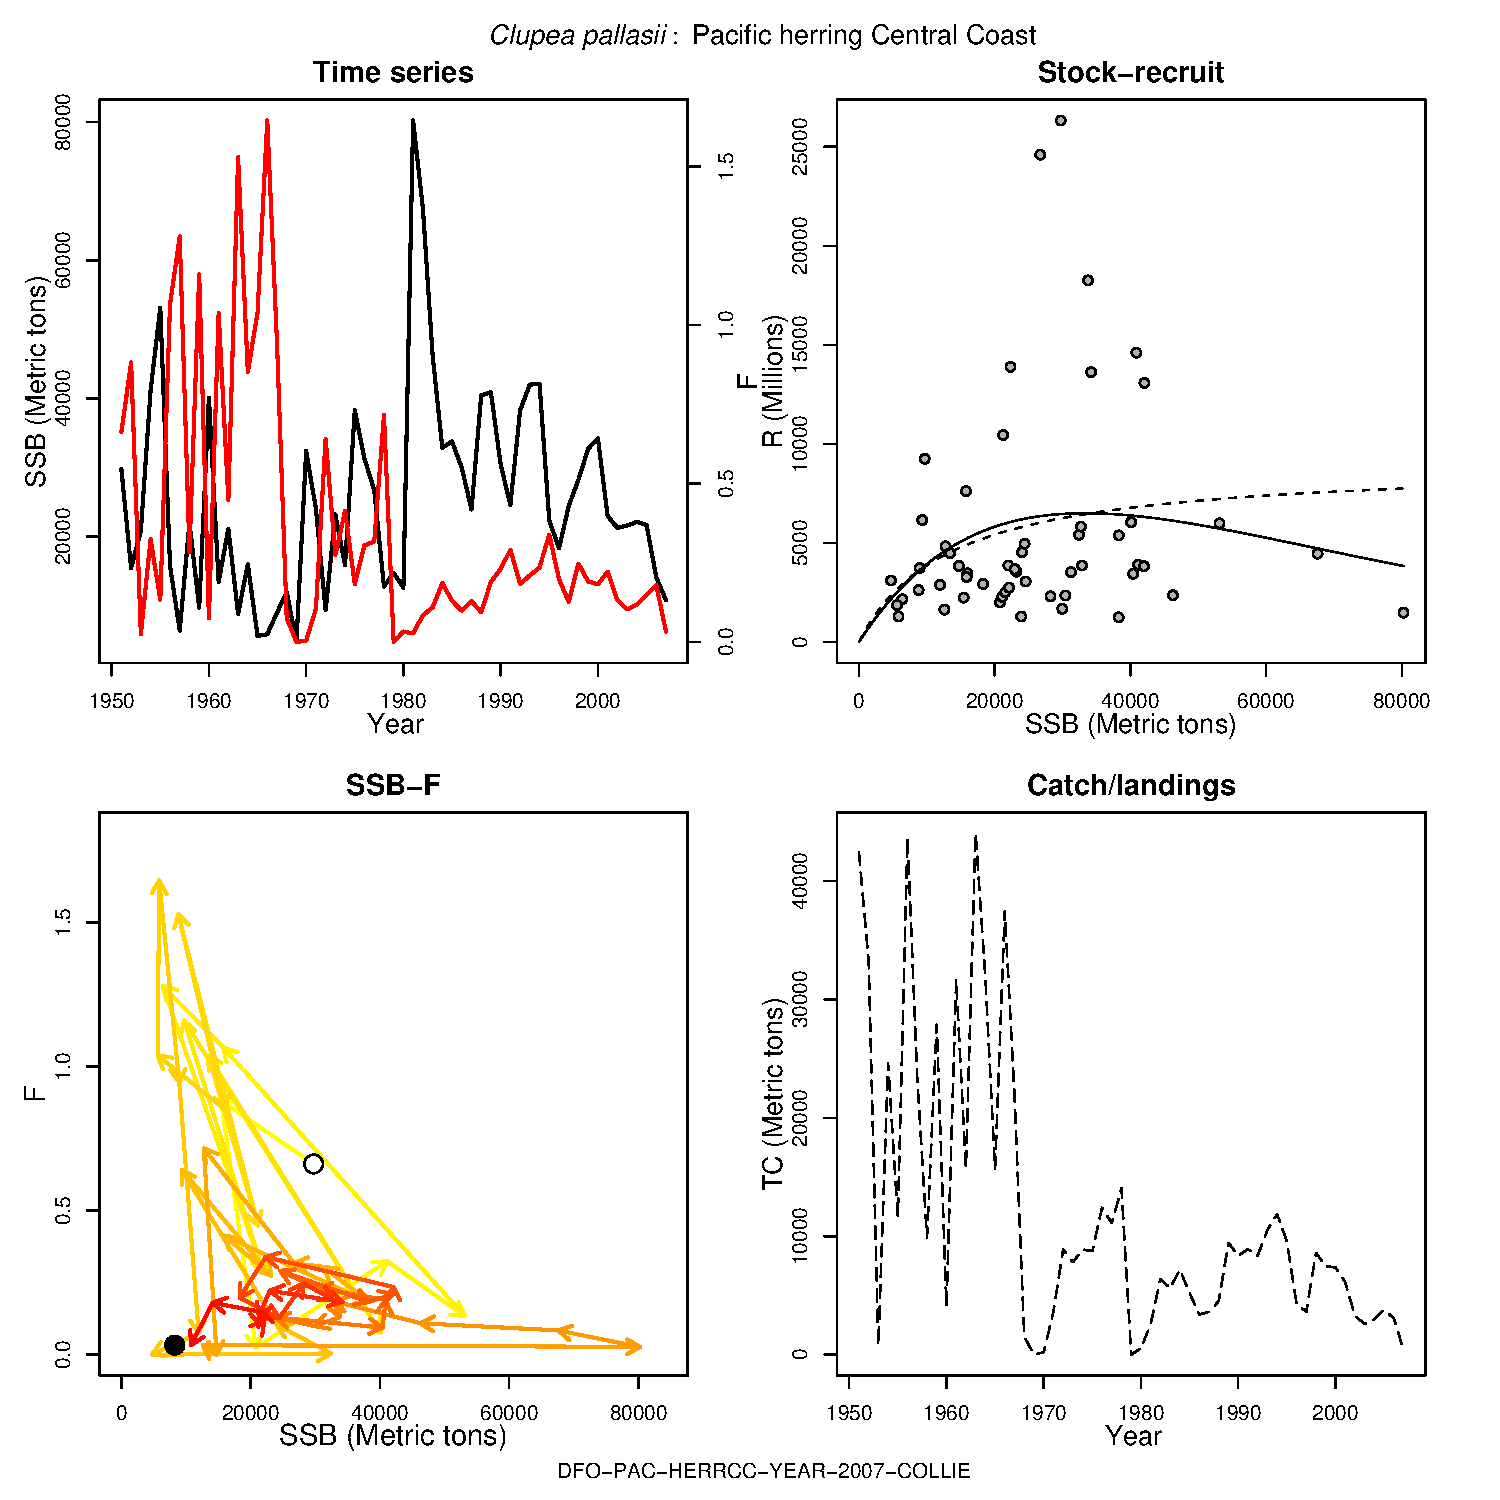
\includegraphics[width=1.2\textwidth]{../R/figures/DFO-PAC-HERRCC-YEAR-2007-COLLIE.pdf}
\end{center}

\subsubsection{Clupea pallasii - Pacific herring}\index{Pacific herring}\index{Clupea pallasii}\index{Clupeidae!Clupea pallasii}
\begin{center}
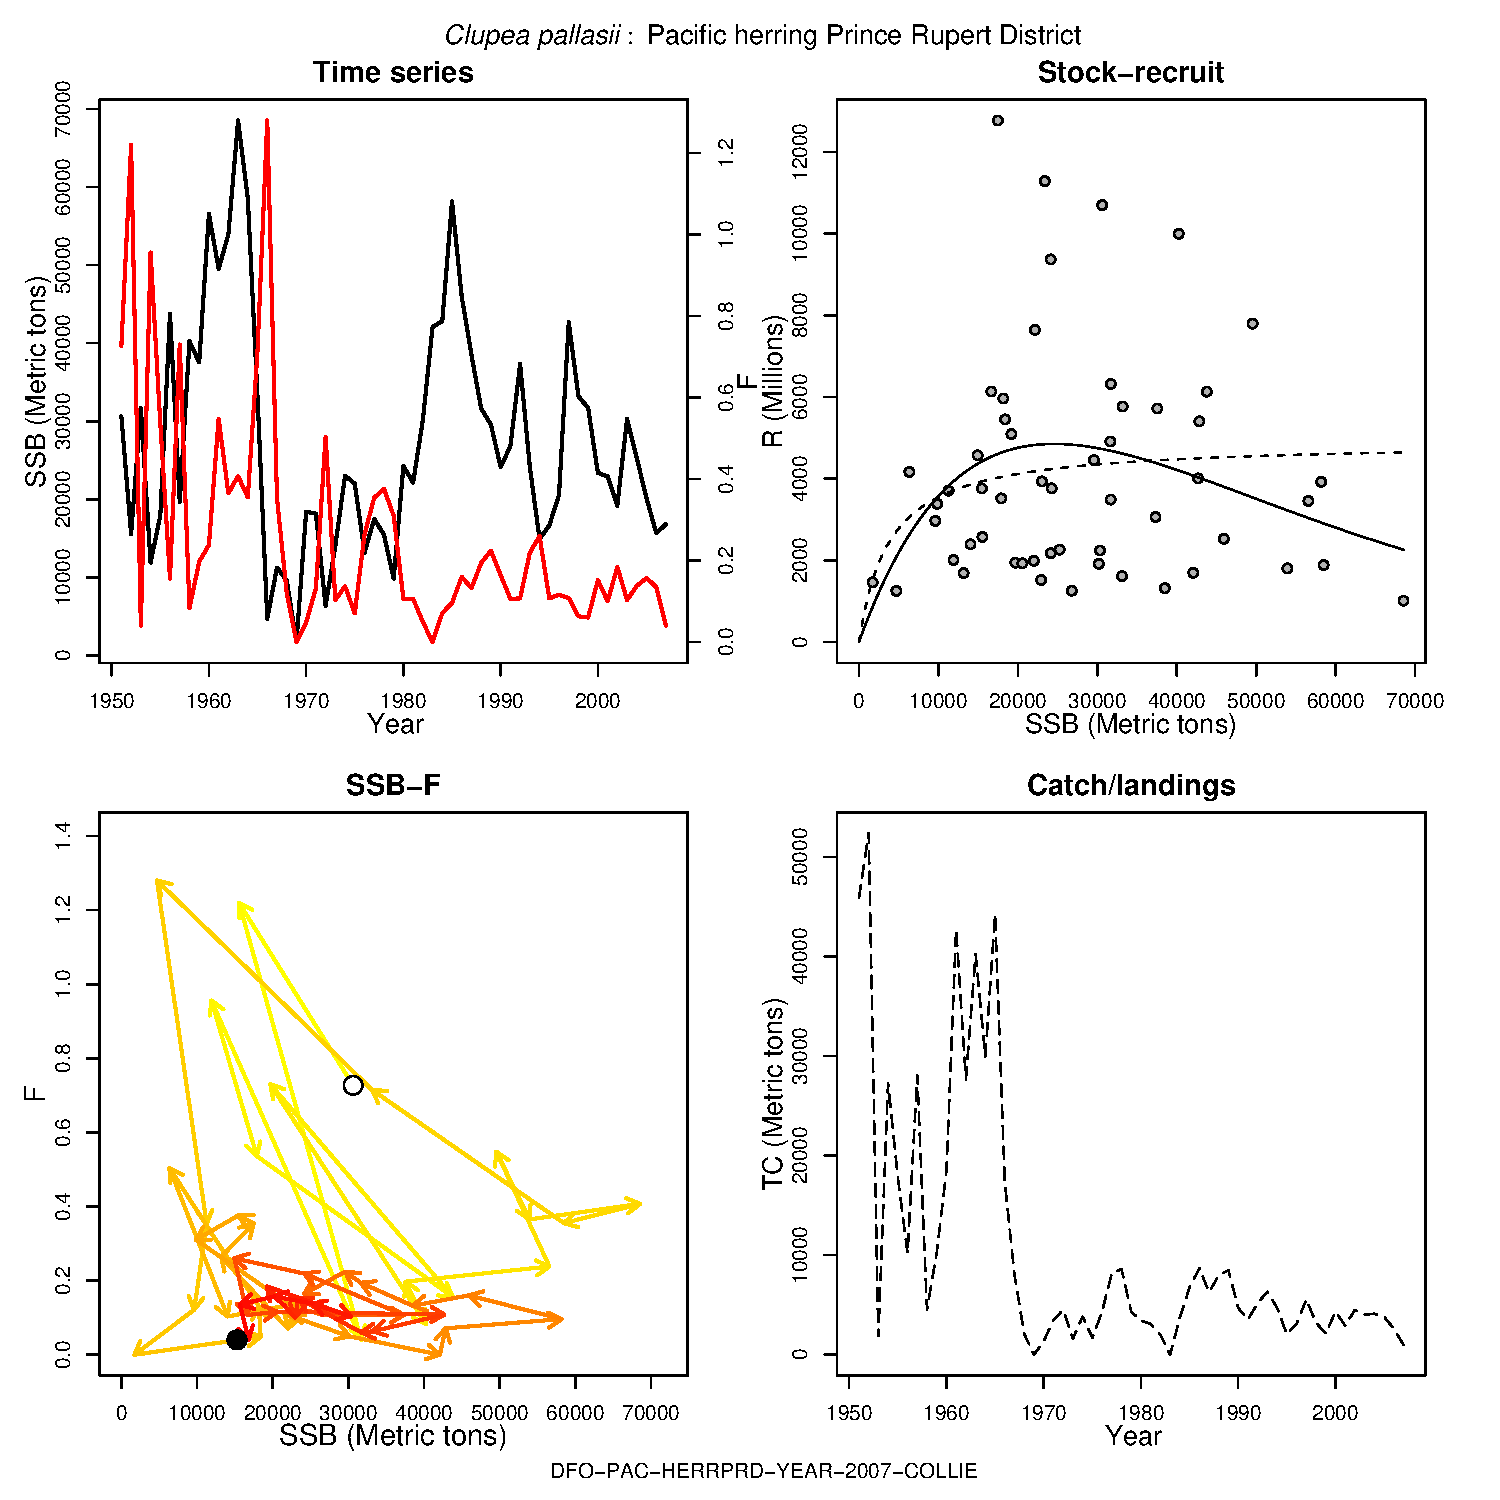
\includegraphics[width=1.2\textwidth]{../R/figures/DFO-PAC-HERRPRD-YEAR-2007-COLLIE.pdf}
\end{center}

\subsubsection{Clupea pallasii - Pacific herring}\index{Pacific herring}\index{Clupea pallasii}\index{Clupeidae!Clupea pallasii}
\begin{center}
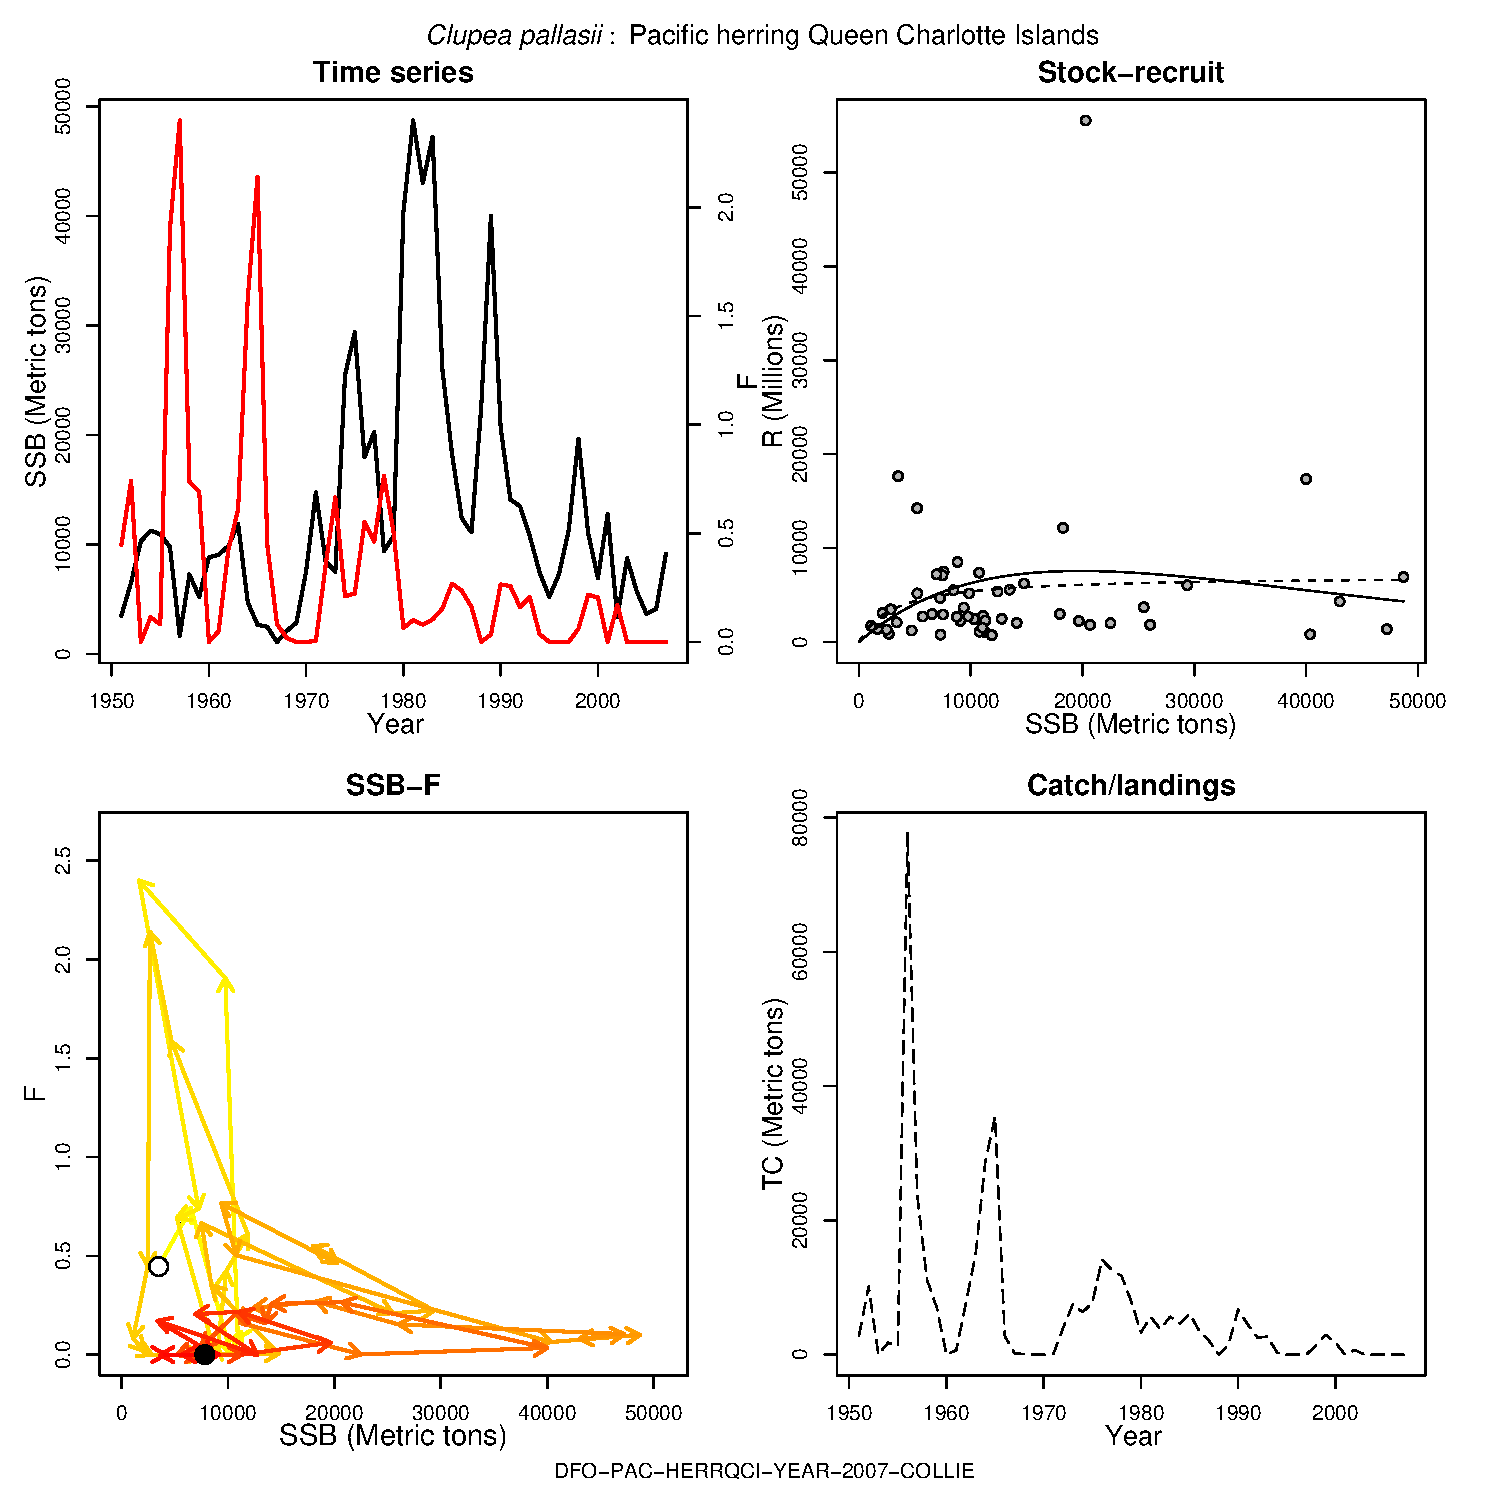
\includegraphics[width=1.2\textwidth]{../R/figures/DFO-PAC-HERRQCI-YEAR-2007-COLLIE.pdf}
\end{center}

\subsubsection{Clupea pallasii - Pacific herring}\index{Pacific herring}\index{Clupea pallasii}\index{Clupeidae!Clupea pallasii}
\begin{center}
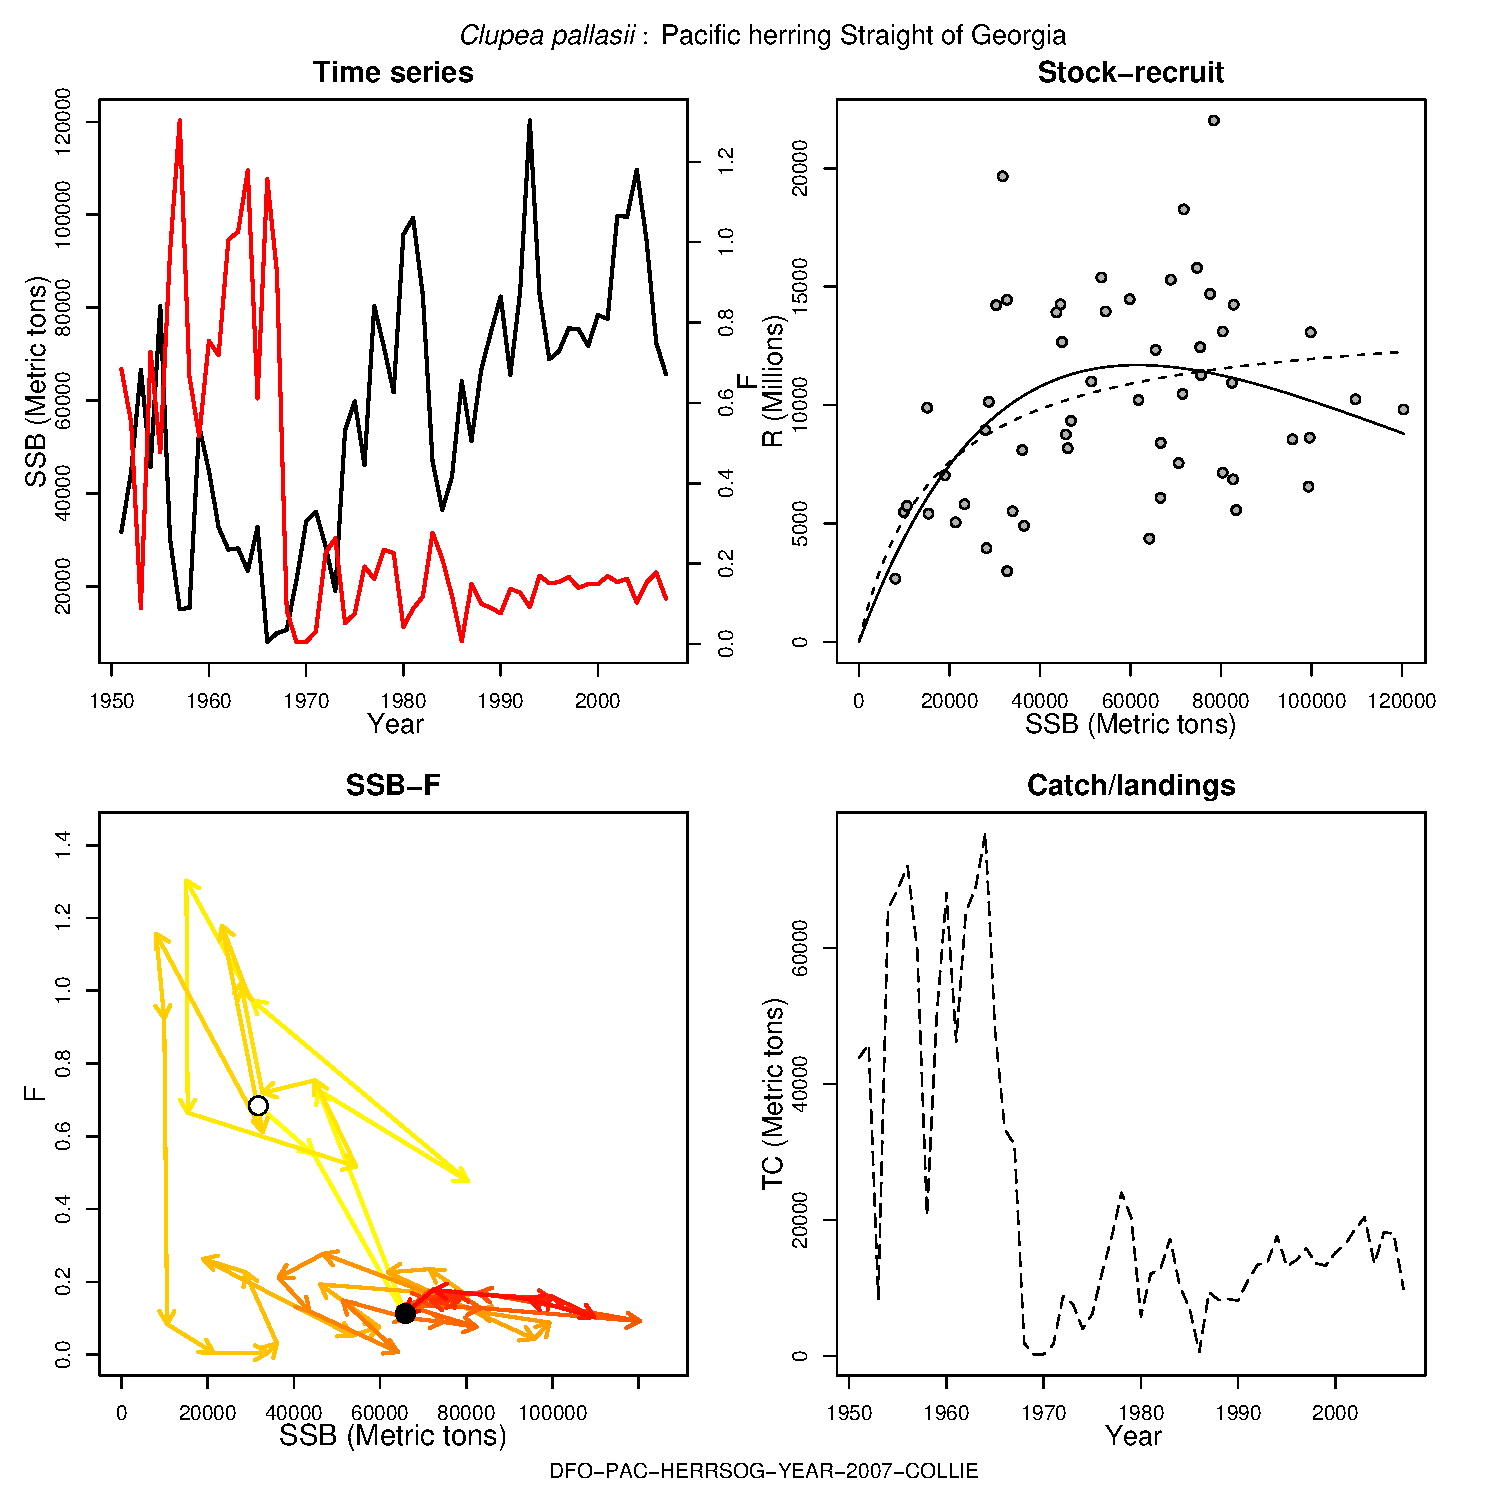
\includegraphics[width=1.2\textwidth]{../R/figures/DFO-PAC-HERRSOG-YEAR-2007-COLLIE.pdf}
\end{center}

\subsubsection{Clupea pallasii - Pacific herring}\index{Pacific herring}\index{Clupea pallasii}\index{Clupeidae!Clupea pallasii}
\begin{center}
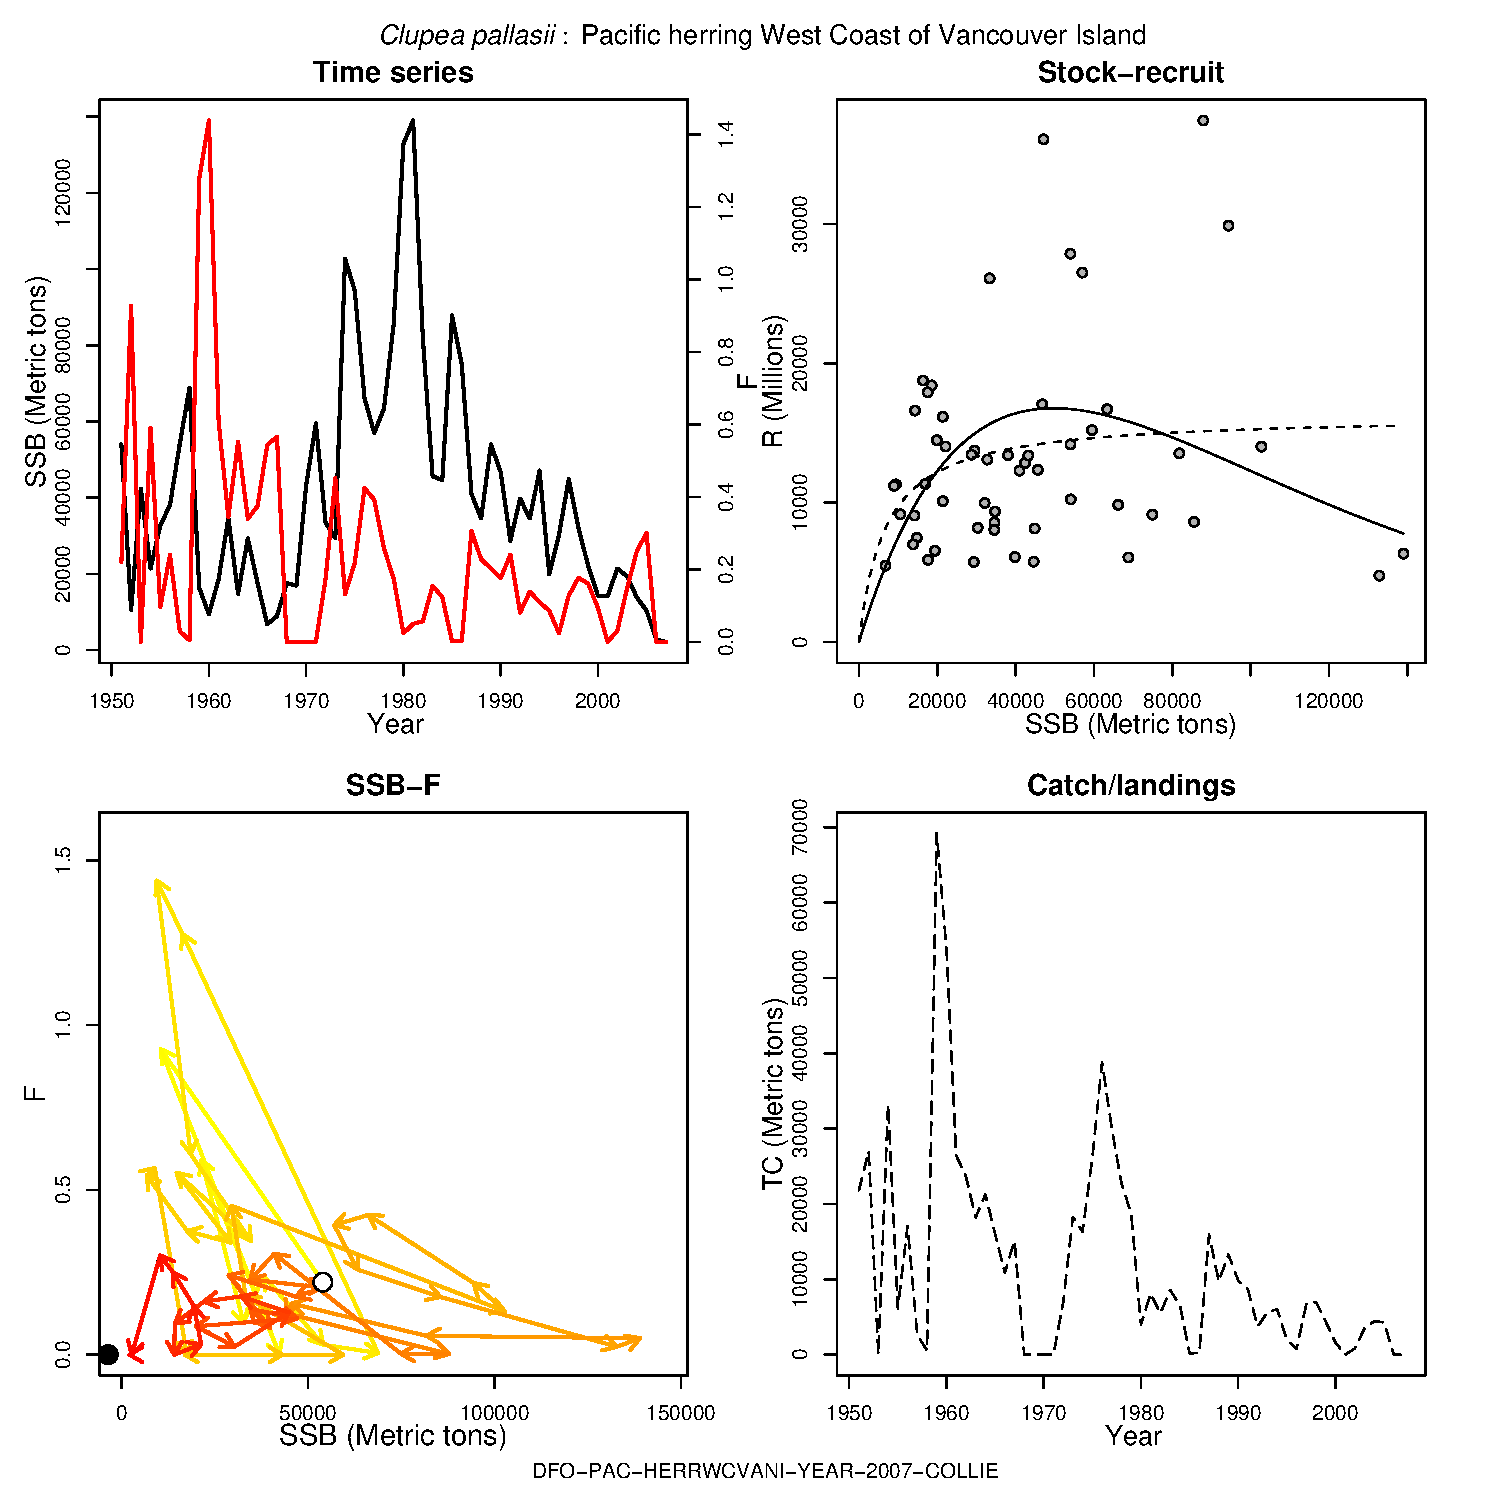
\includegraphics[width=1.2\textwidth]{../R/figures/DFO-PAC-HERRWCVANI-YEAR-2007-COLLIE.pdf}
\end{center}

\subsubsection{Sprattus sprattus - Sprat}\index{Sprat}\index{Sprattus sprattus}\index{Clupeidae!Sprattus sprattus}
\begin{center}
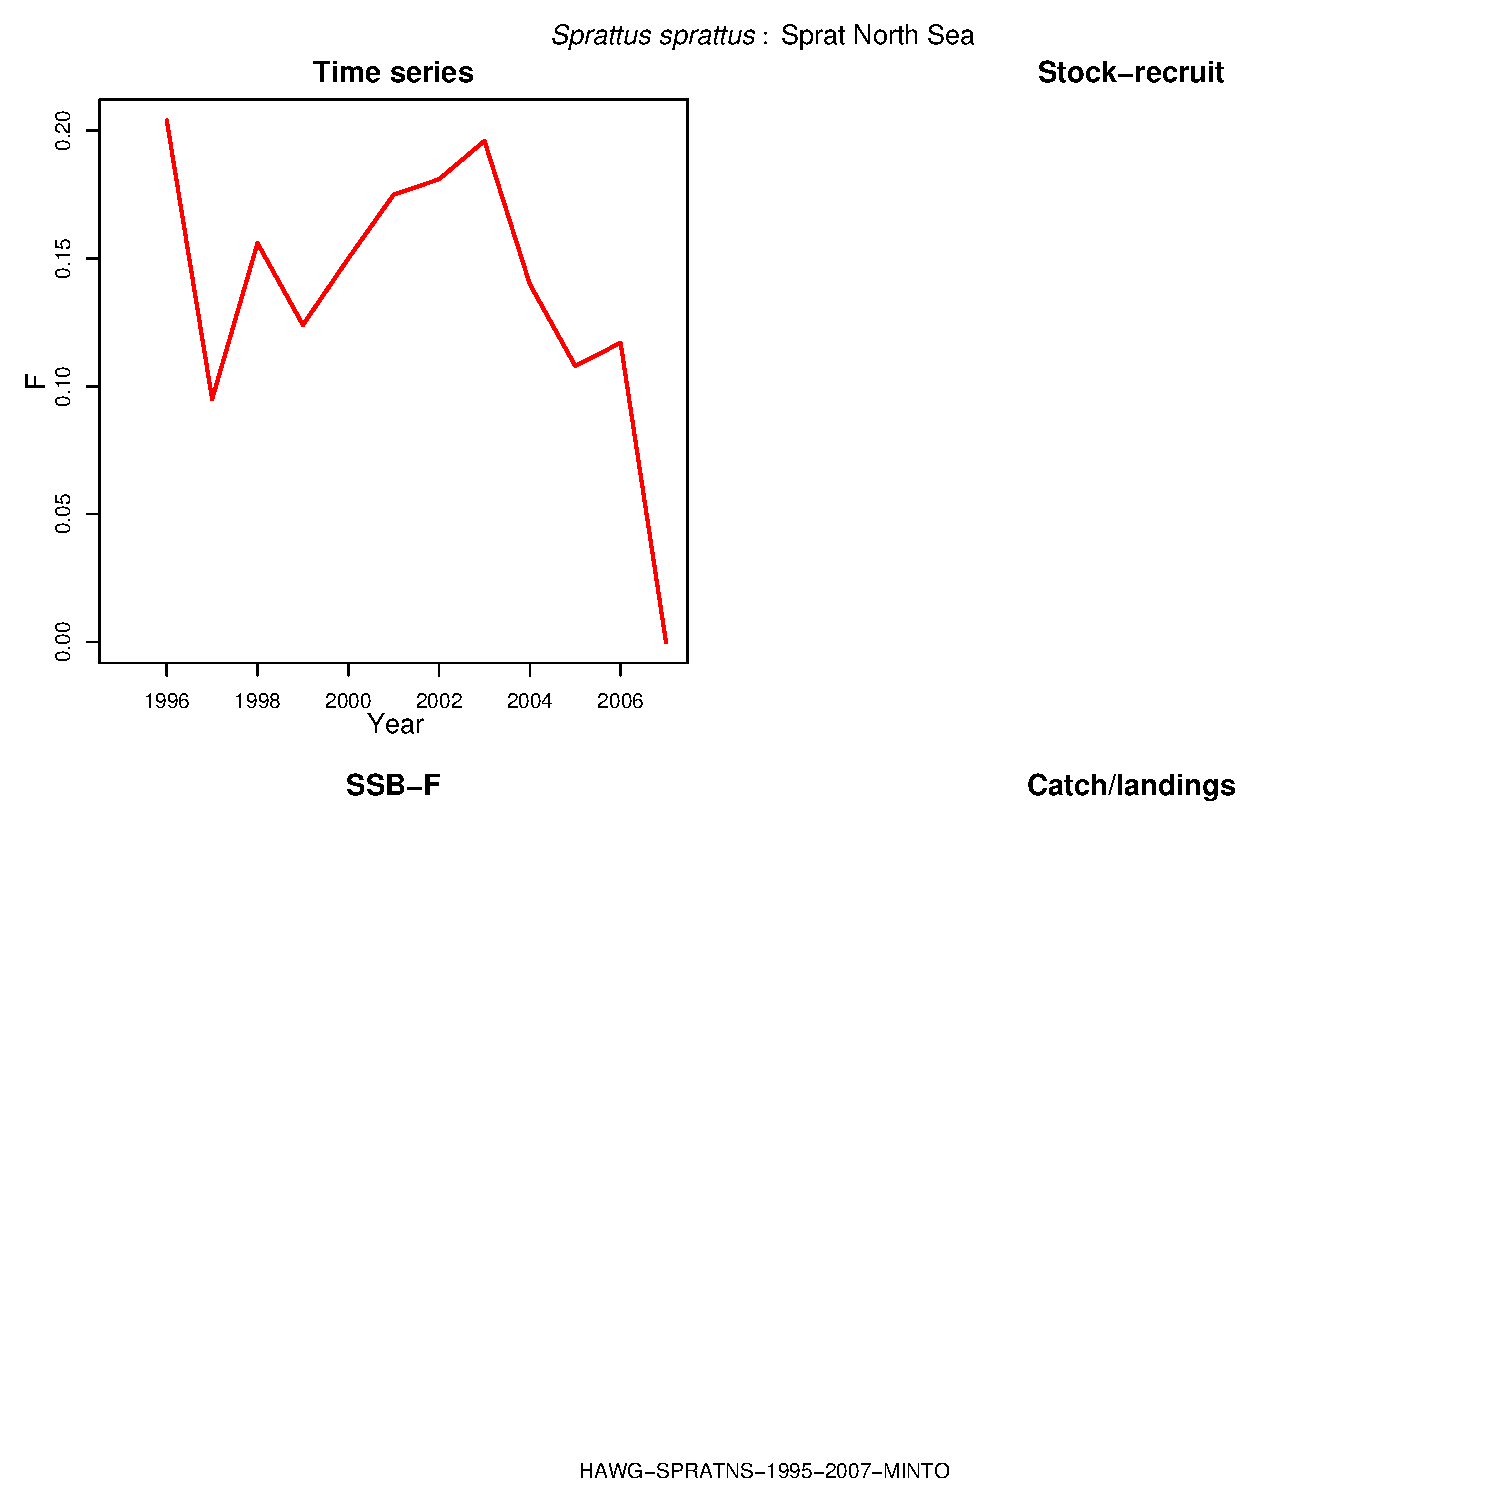
\includegraphics[width=1.2\textwidth]{../R/figures/HAWG-SPRATNS-1995-2007-MINTO.pdf}
\end{center}

\section{Decapoda}\index{Decapoda}

\subsection{Lithodidae}\index{Lithodidae}\index{Decapoda!Lithodidae}

\subsection{Nephropidae}\index{Nephropidae}\index{Decapoda!Nephropidae}

\subsubsection{Homarus americanus - American lobster}\index{American lobster}\index{Homarus americanus}\index{Nephropidae!Homarus americanus}
\begin{center}
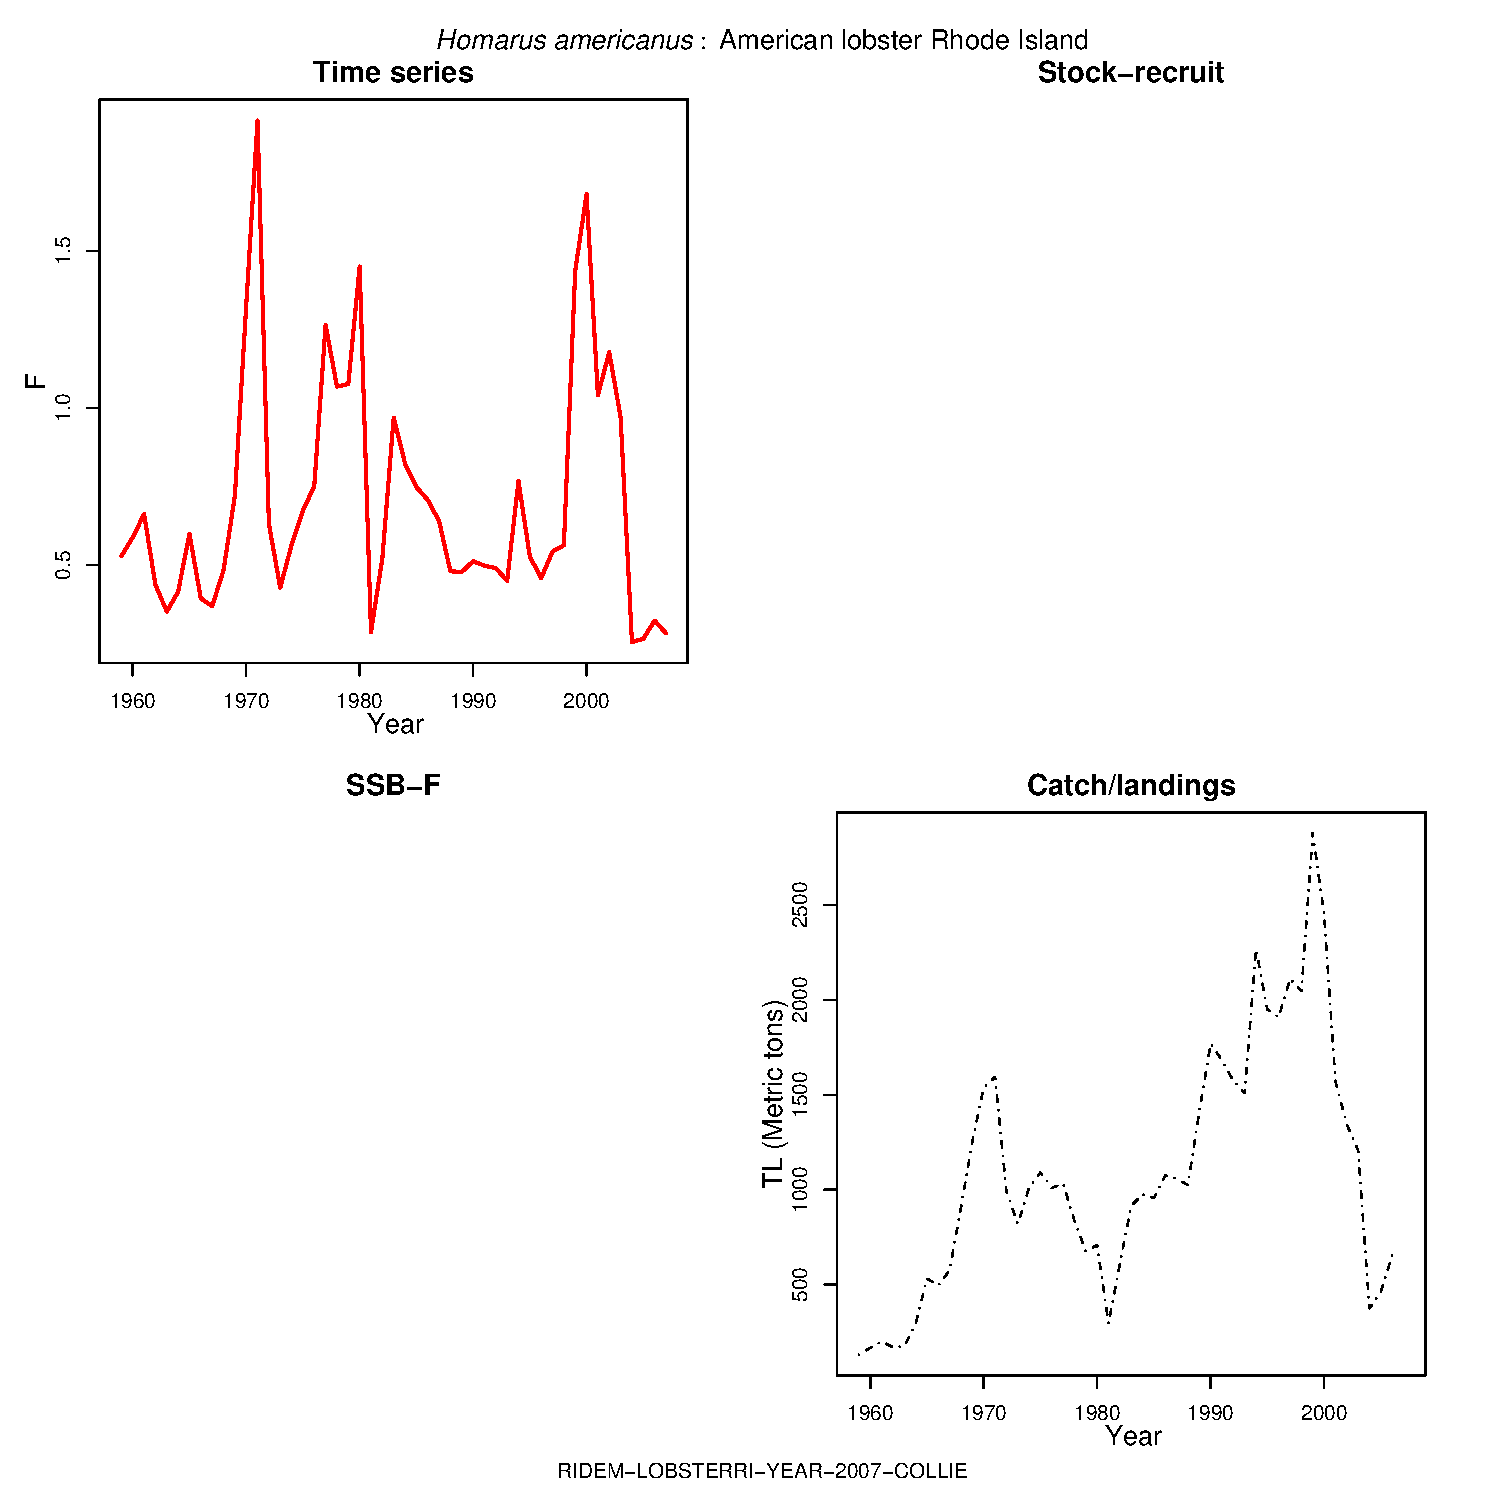
\includegraphics[width=1.2\textwidth]{../R/figures/RIDEM-LOBSTERRI-YEAR-2007-COLLIE.pdf}
\end{center}

\subsection{Oregoniidae}\index{Oregoniidae}\index{Decapoda!Oregoniidae}

\subsubsection{Chionoecetes opilio - Snow crab}\index{Snow crab}\index{Chionoecetes opilio}\index{Oregoniidae!Chionoecetes opilio}
\begin{center}
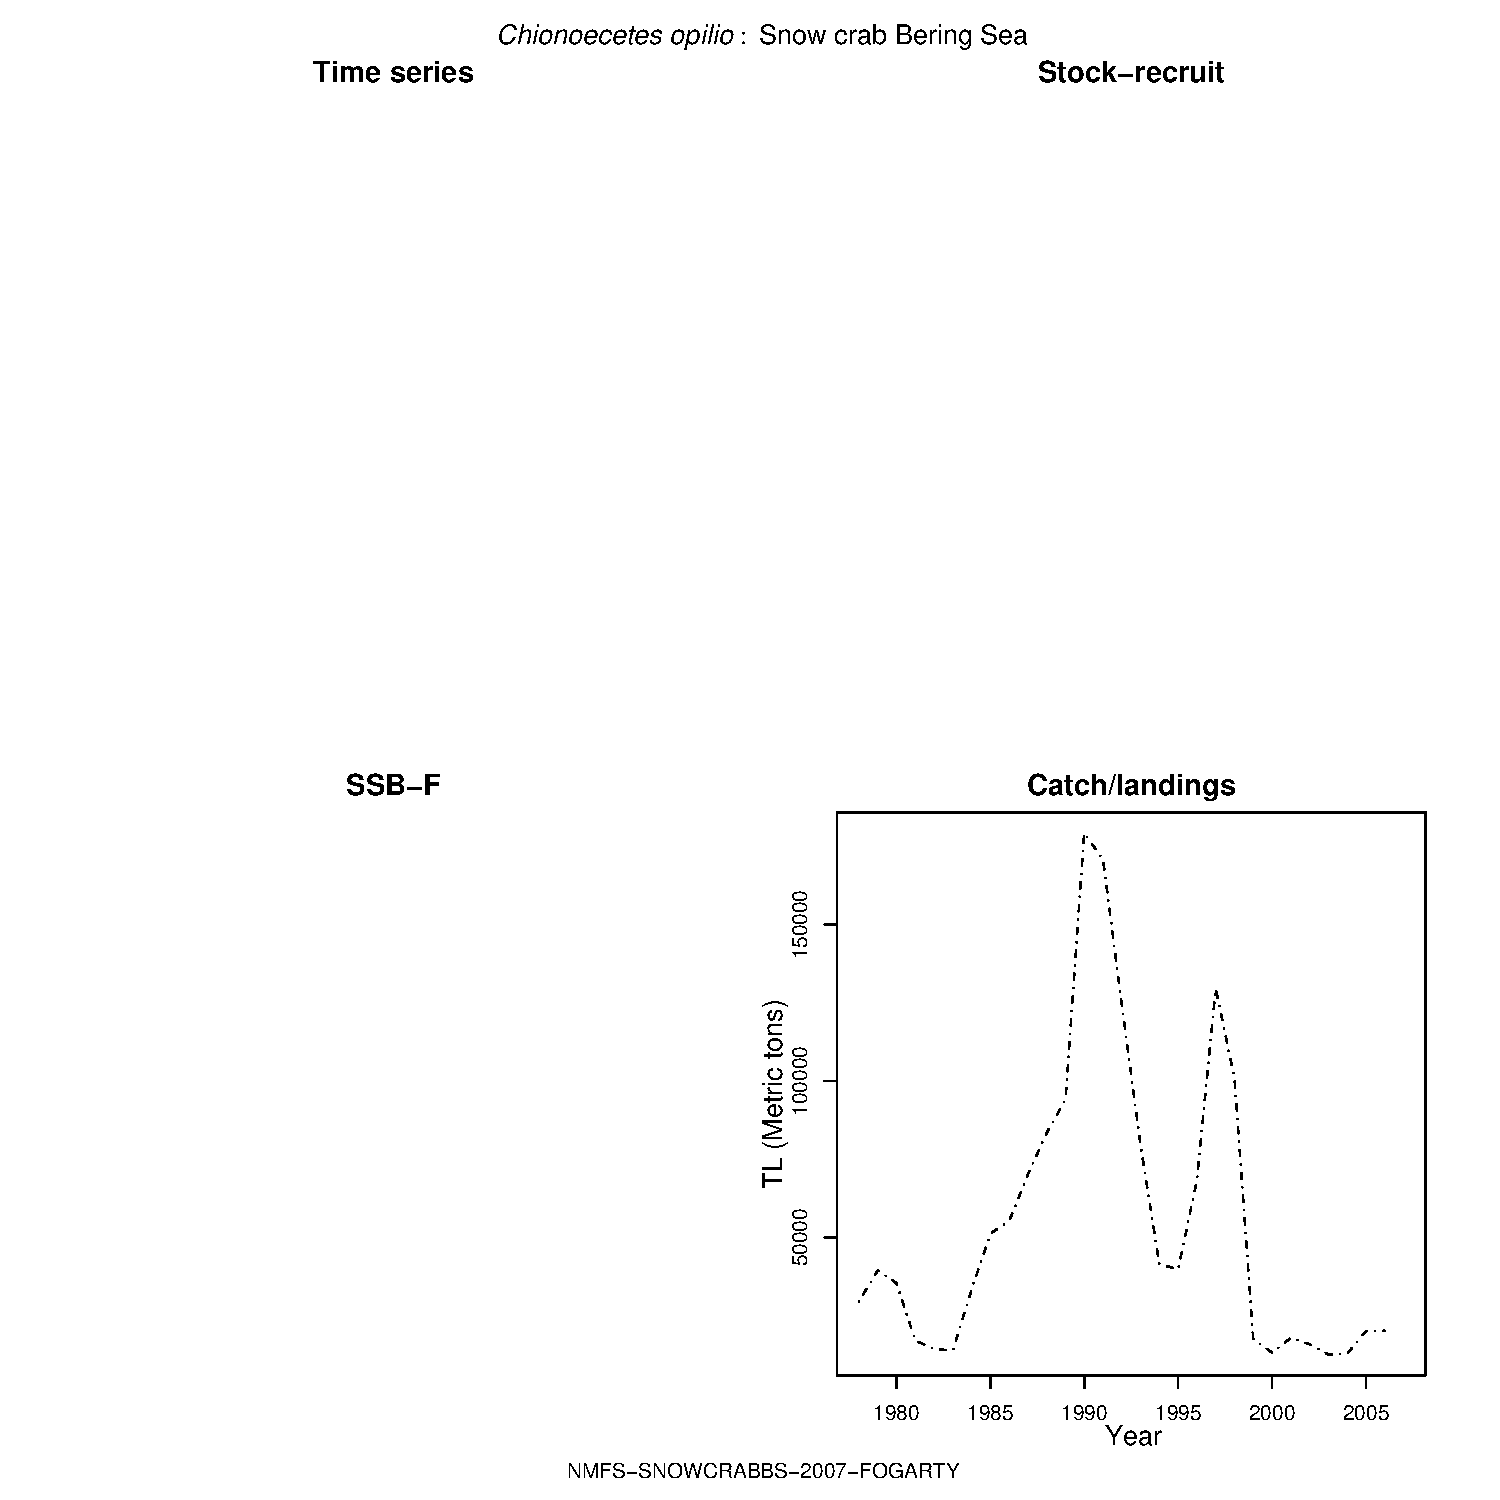
\includegraphics[width=1.2\textwidth]{../R/figures/NMFS-SNOWCRABBS-2007-FOGARTY.pdf}
\end{center}

\section{Gadiformes}\index{Gadiformes}

\subsection{Gadidae}\index{Gadidae}\index{Gadiformes!Gadidae}

\subsubsection{Gadus macrocephalus - Pacific cod}\index{Pacific cod}\index{Gadus macrocephalus}\index{Gadidae!Gadus macrocephalus}
\begin{center}
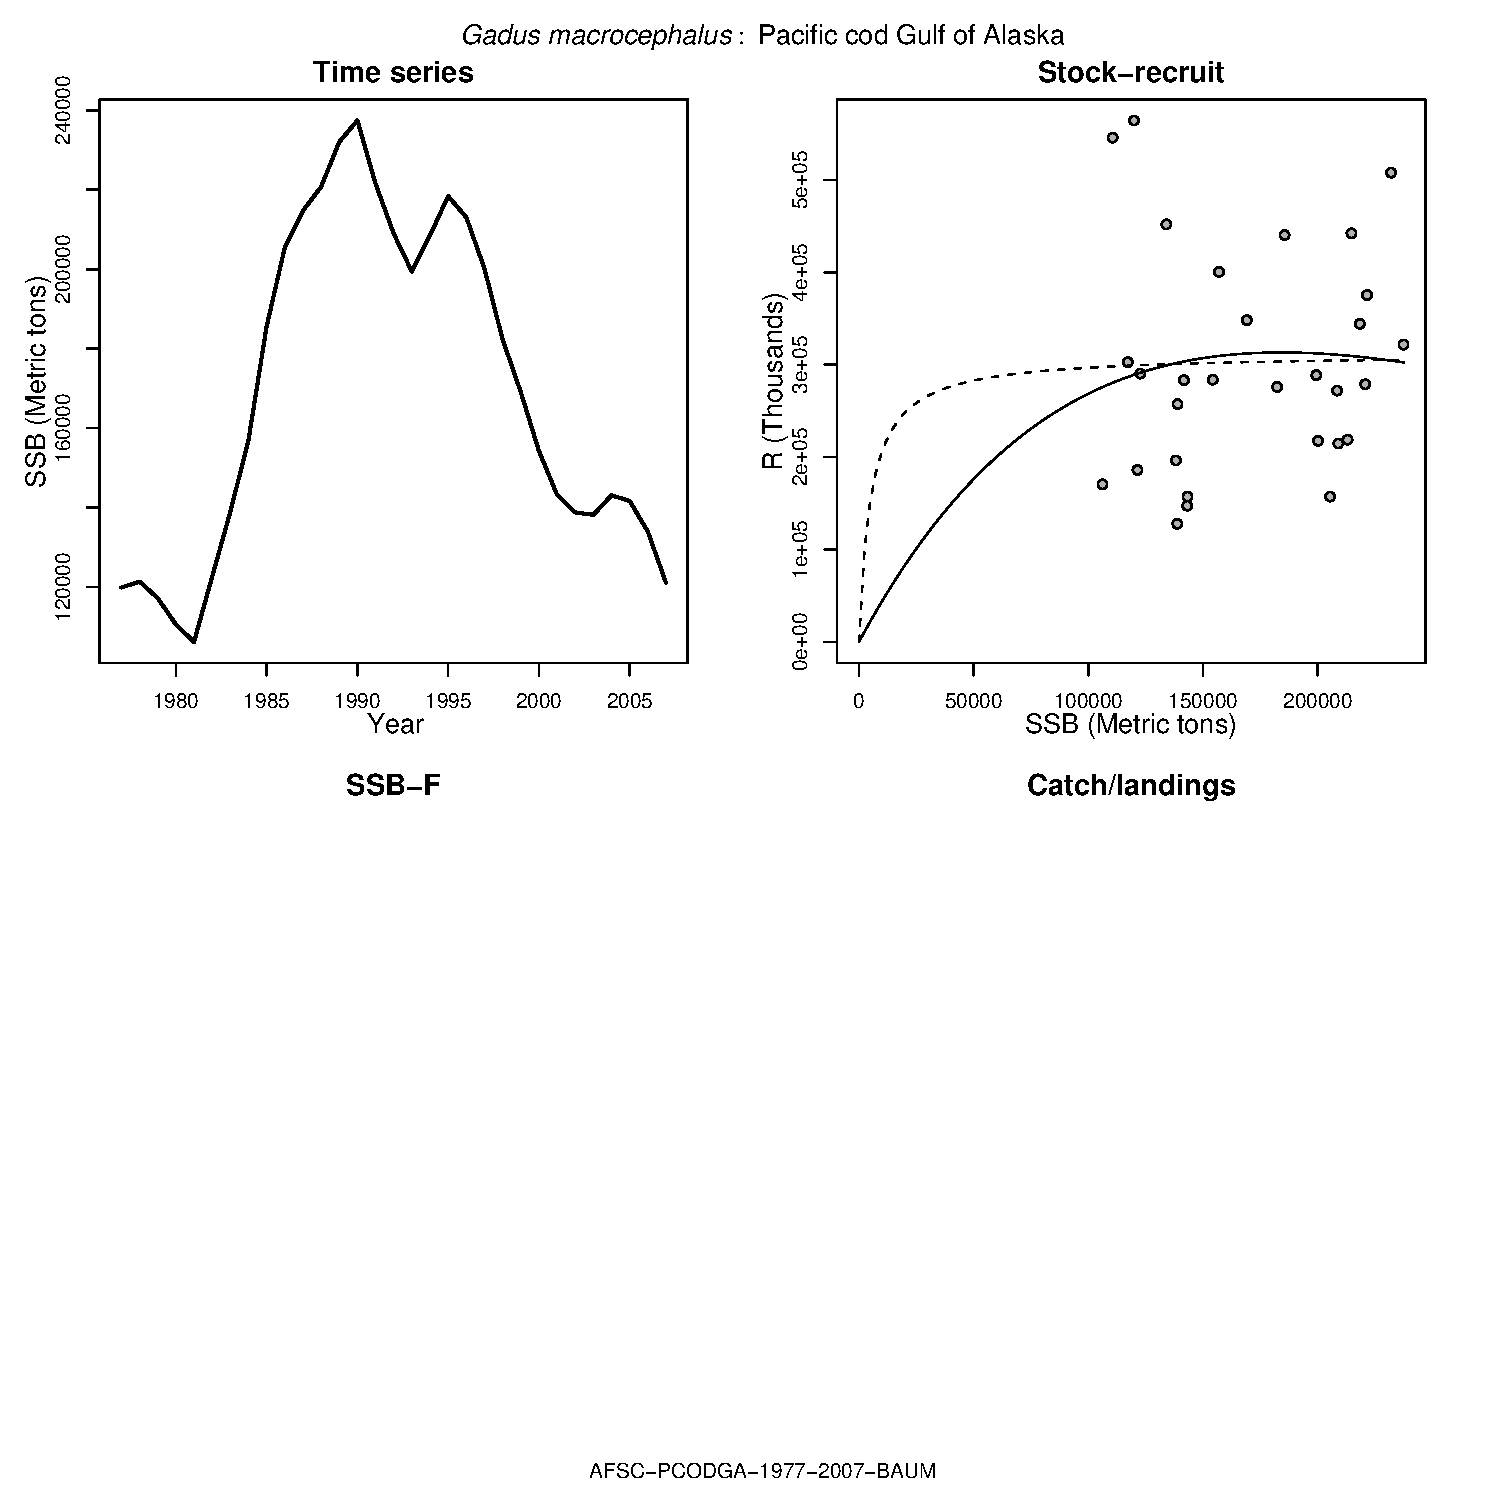
\includegraphics[width=1.2\textwidth]{../R/figures/AFSC-PCODGA-1977-2007-BAUM.pdf}
\end{center}

\subsubsection{Gadus macrocephalus - Pacific cod}\index{Pacific cod}\index{Gadus macrocephalus}\index{Gadidae!Gadus macrocephalus}
\begin{center}
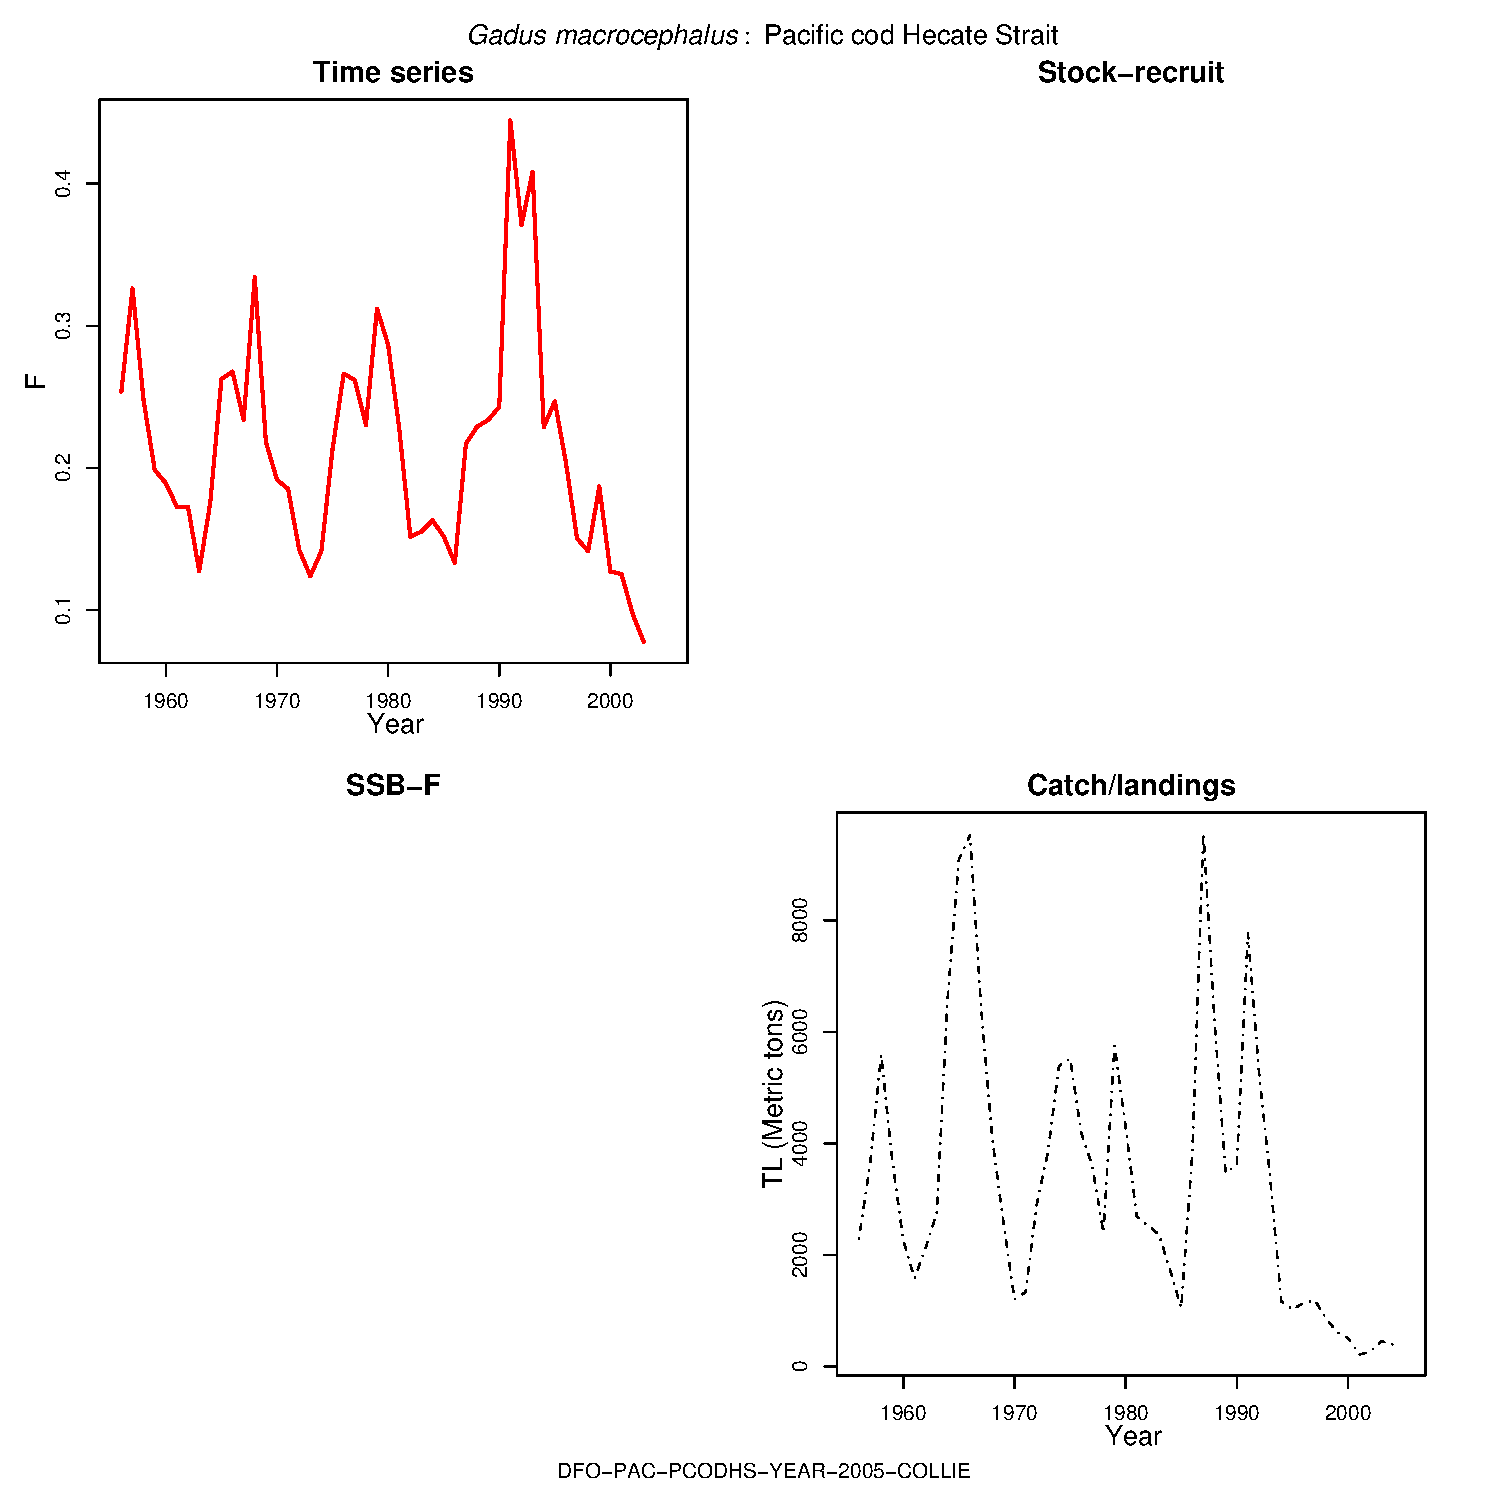
\includegraphics[width=1.2\textwidth]{../R/figures/DFO-PAC-PCODHS-YEAR-2005-COLLIE.pdf}
\end{center}

\subsubsection{Gadus macrocephalus - Pacific cod}\index{Pacific cod}\index{Gadus macrocephalus}\index{Gadidae!Gadus macrocephalus}
\begin{center}
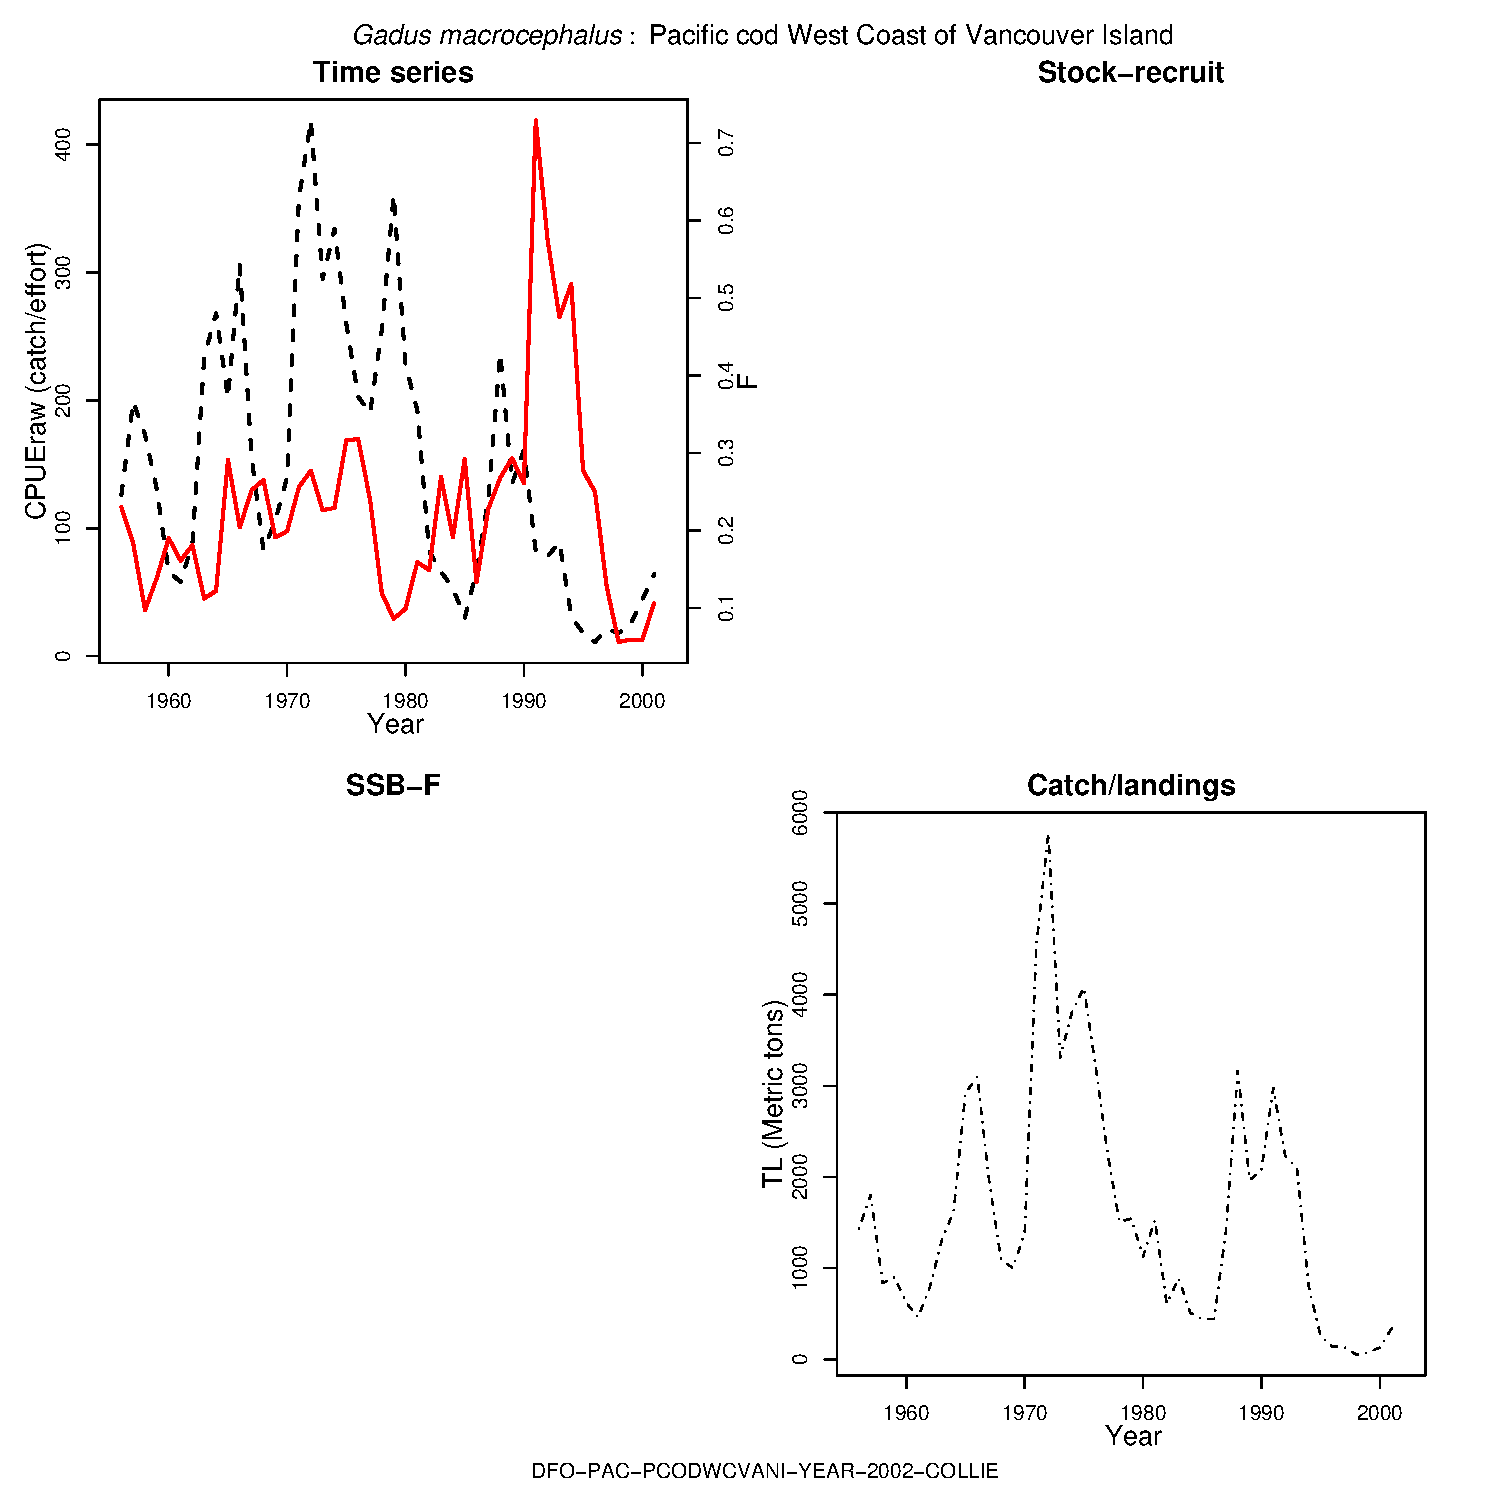
\includegraphics[width=1.2\textwidth]{../R/figures/DFO-PAC-PCODWCVANI-YEAR-2002-COLLIE.pdf}
\end{center}

\subsubsection{Gadus macrocephalus - Pacific cod}\index{Pacific cod}\index{Gadus macrocephalus}\index{Gadidae!Gadus macrocephalus}
\begin{center}
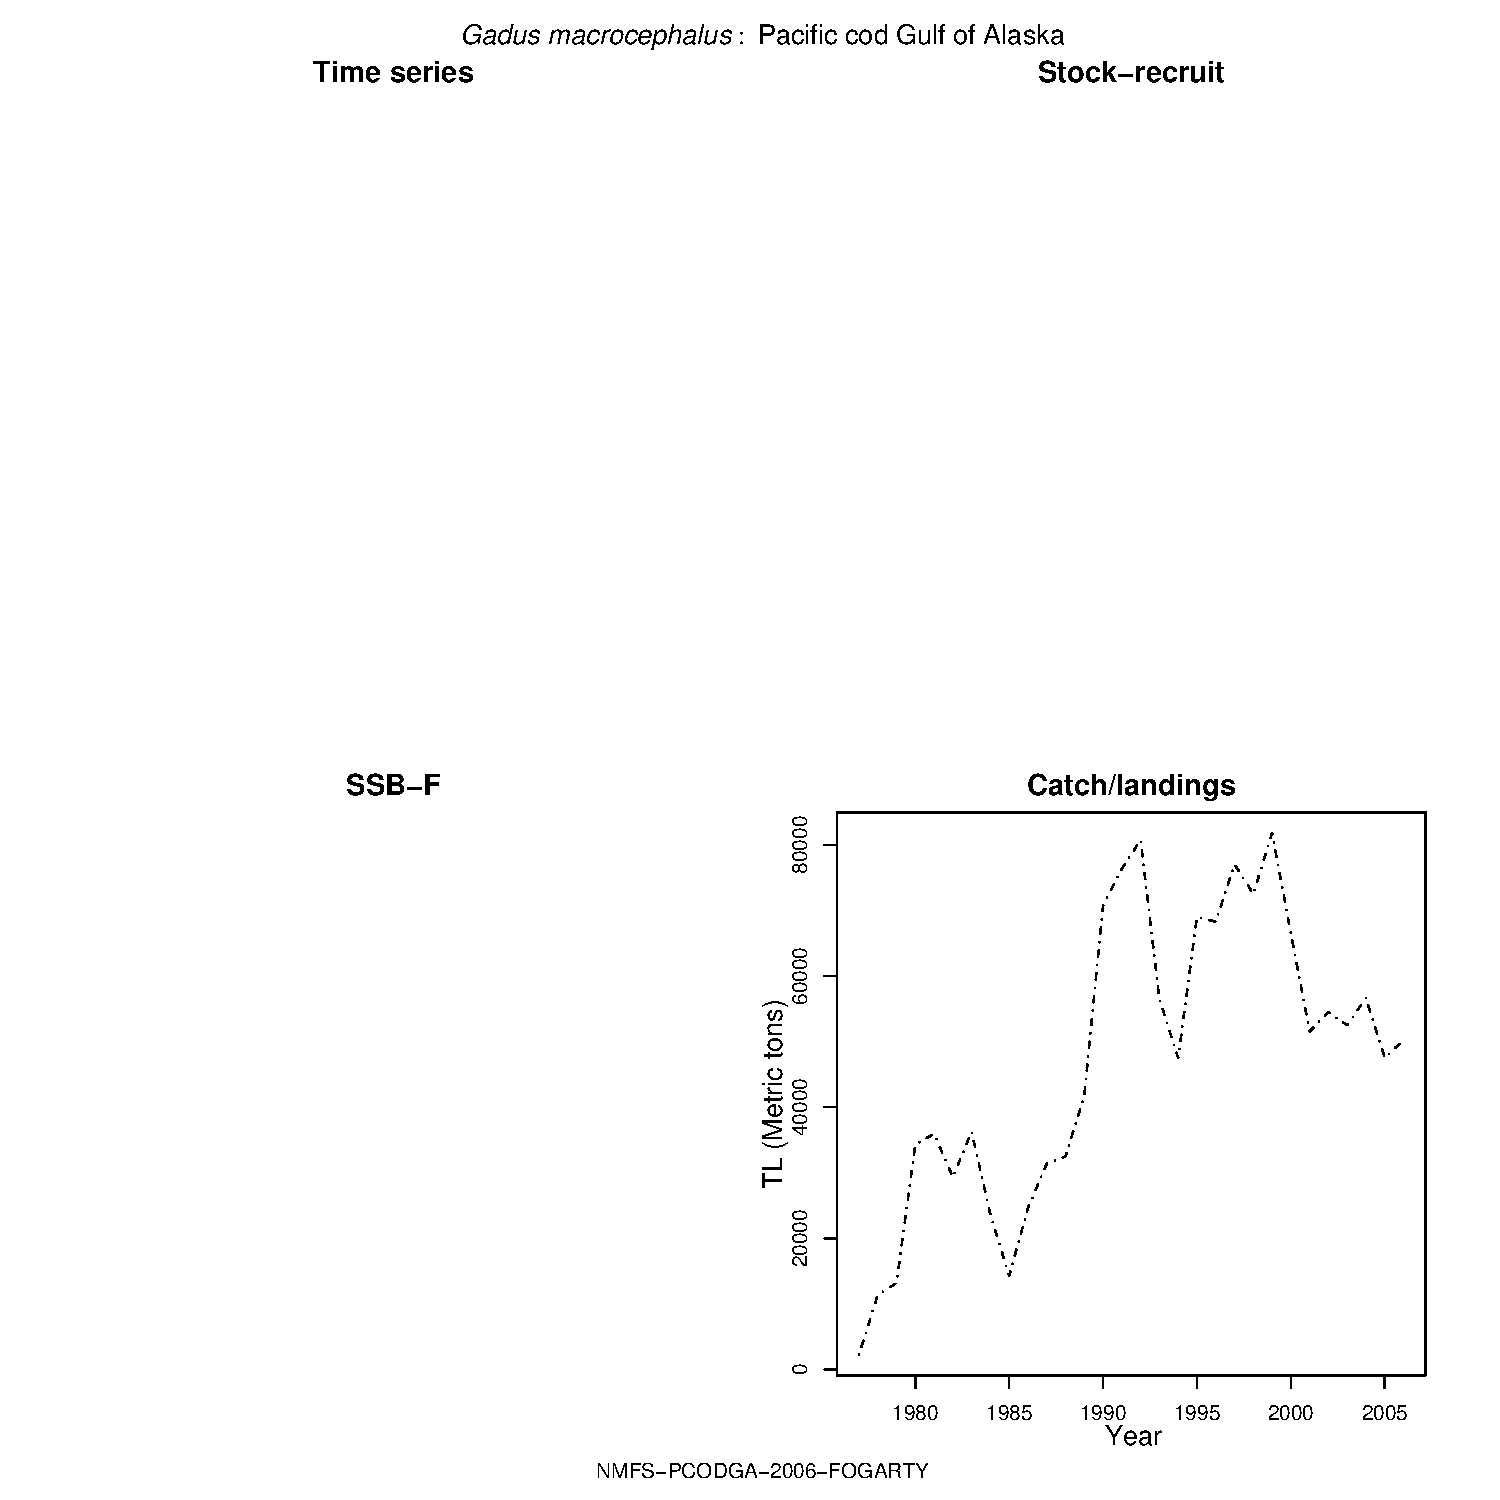
\includegraphics[width=1.2\textwidth]{../R/figures/NMFS-PCODGA-2006-FOGARTY.pdf}
\end{center}

\subsubsection{Gadus macrocephalus - Pacific cod}\index{Pacific cod}\index{Gadus macrocephalus}\index{Gadidae!Gadus macrocephalus}
\begin{center}
\includegraphics[width=1.2\textwidth]{../R/figures/PHONYassessorid-PCODGA-1975-2000-MYERS.pdf}
\end{center}

\subsubsection{Gadus macrocephalus - Pacific cod}\index{Pacific cod}\index{Gadus macrocephalus}\index{Gadidae!Gadus macrocephalus}
\begin{center}
\includegraphics[width=1.2\textwidth]{../R/figures/PHONYassessorid-PCODHS-1956-1989-MYERS.pdf}
\end{center}

\subsubsection{Gadus morhua - Atlantic cod}\index{Atlantic cod}\index{Gadus morhua}\index{Gadidae!Gadus morhua}
\begin{center}
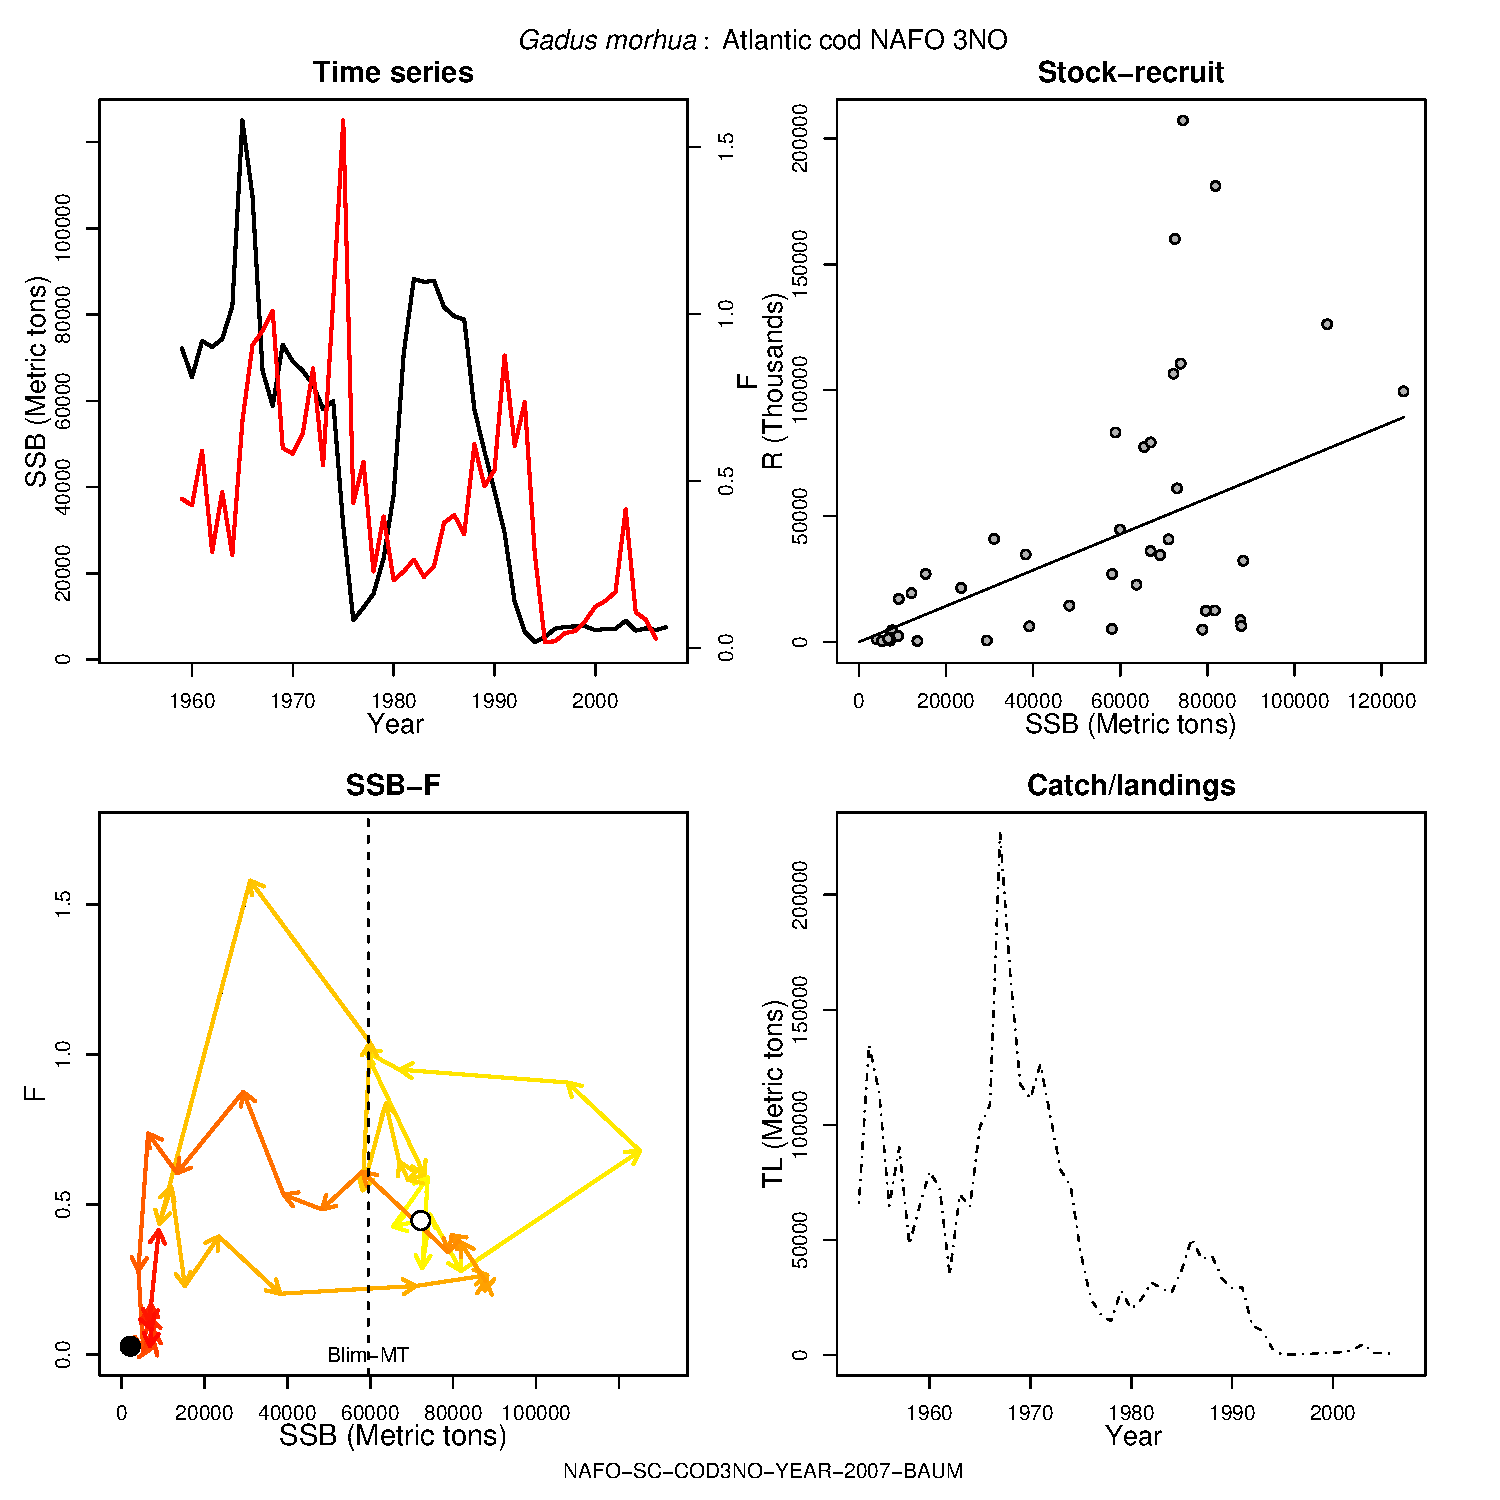
\includegraphics[width=1.2\textwidth]{../R/figures/NAFO-SC-COD3NO-YEAR-2007-BAUM.pdf}
\end{center}

\subsubsection{Gadus morhua - Atlantic cod}\index{Atlantic cod}\index{Gadus morhua}\index{Gadidae!Gadus morhua}
\begin{center}
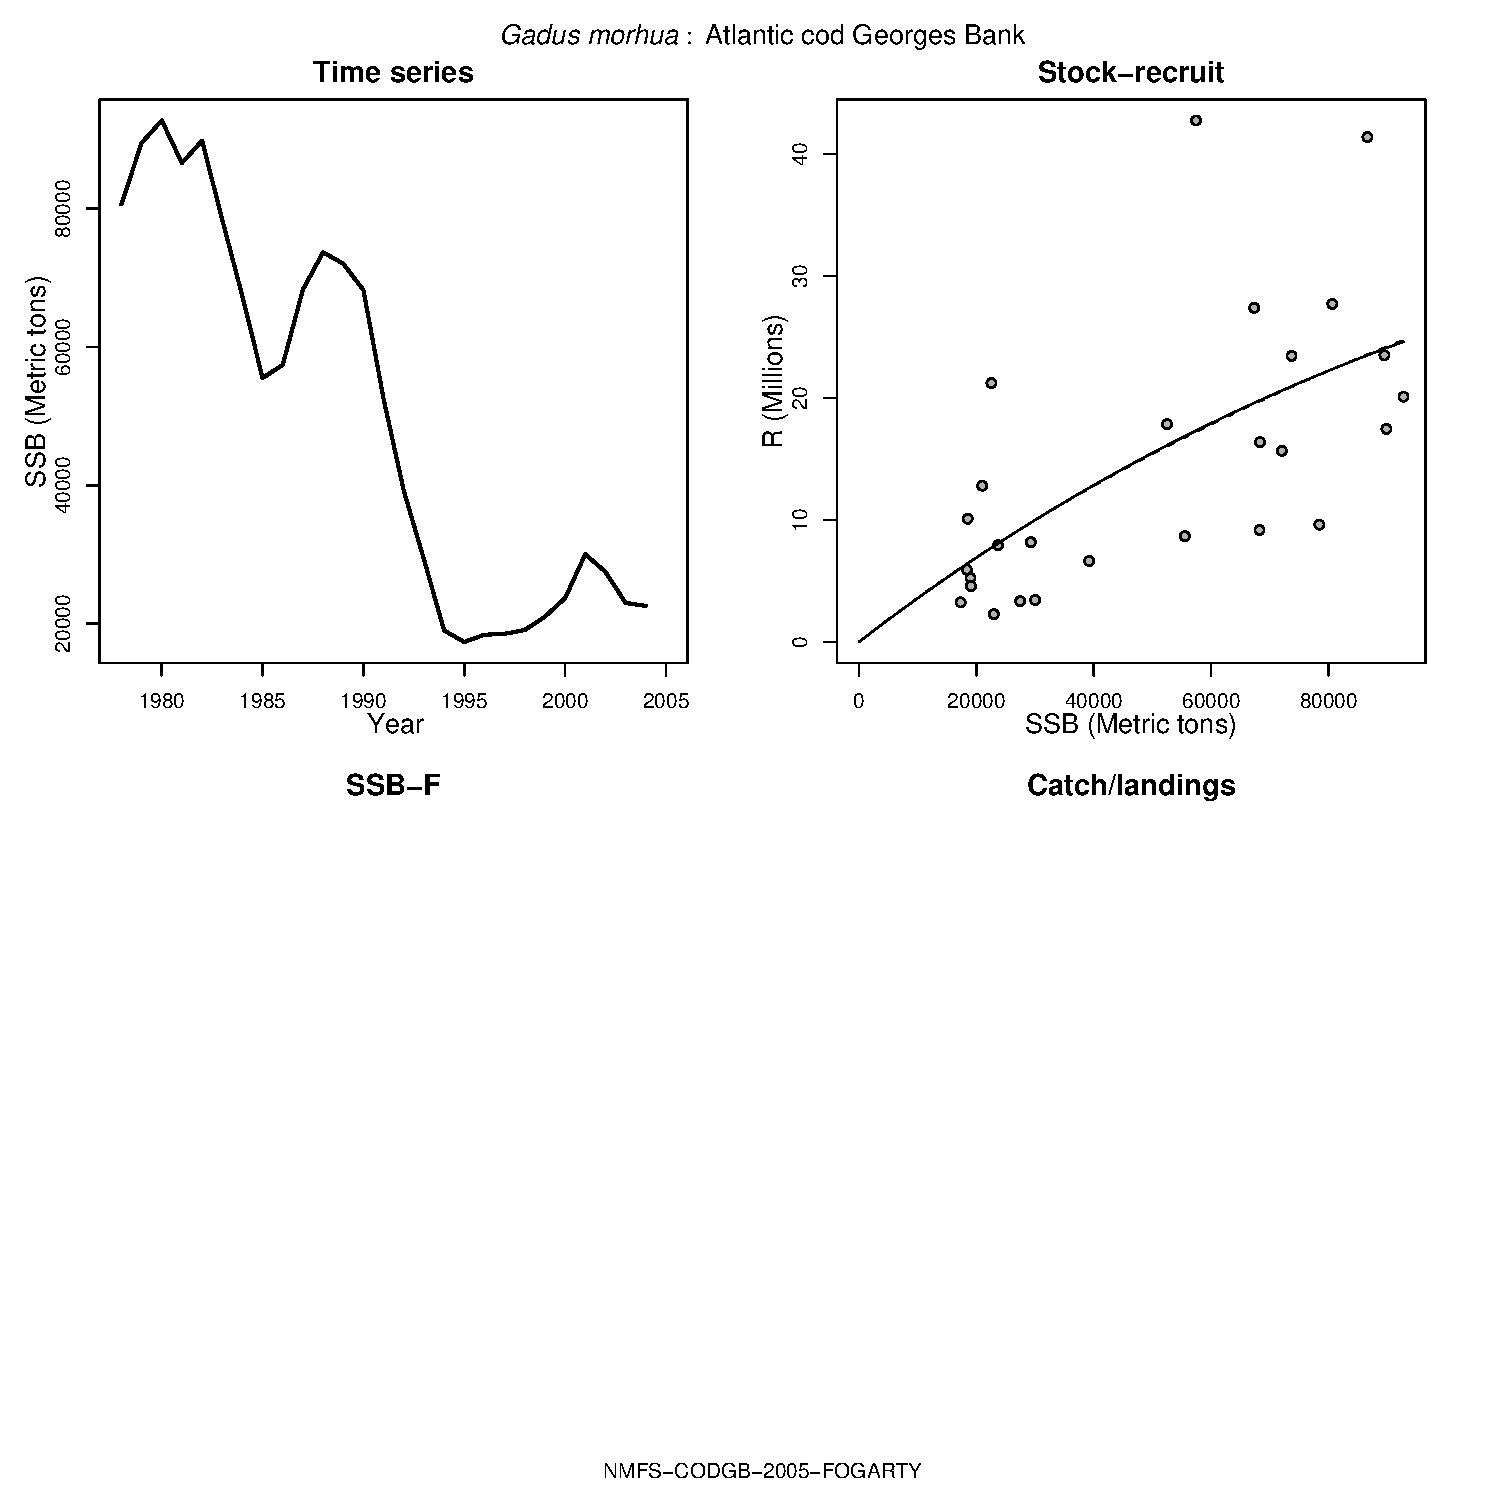
\includegraphics[width=1.2\textwidth]{../R/figures/NMFS-CODGB-2005-FOGARTY.pdf}
\end{center}

\subsubsection{Gadus morhua - Atlantic cod}\index{Atlantic cod}\index{Gadus morhua}\index{Gadidae!Gadus morhua}
\begin{center}
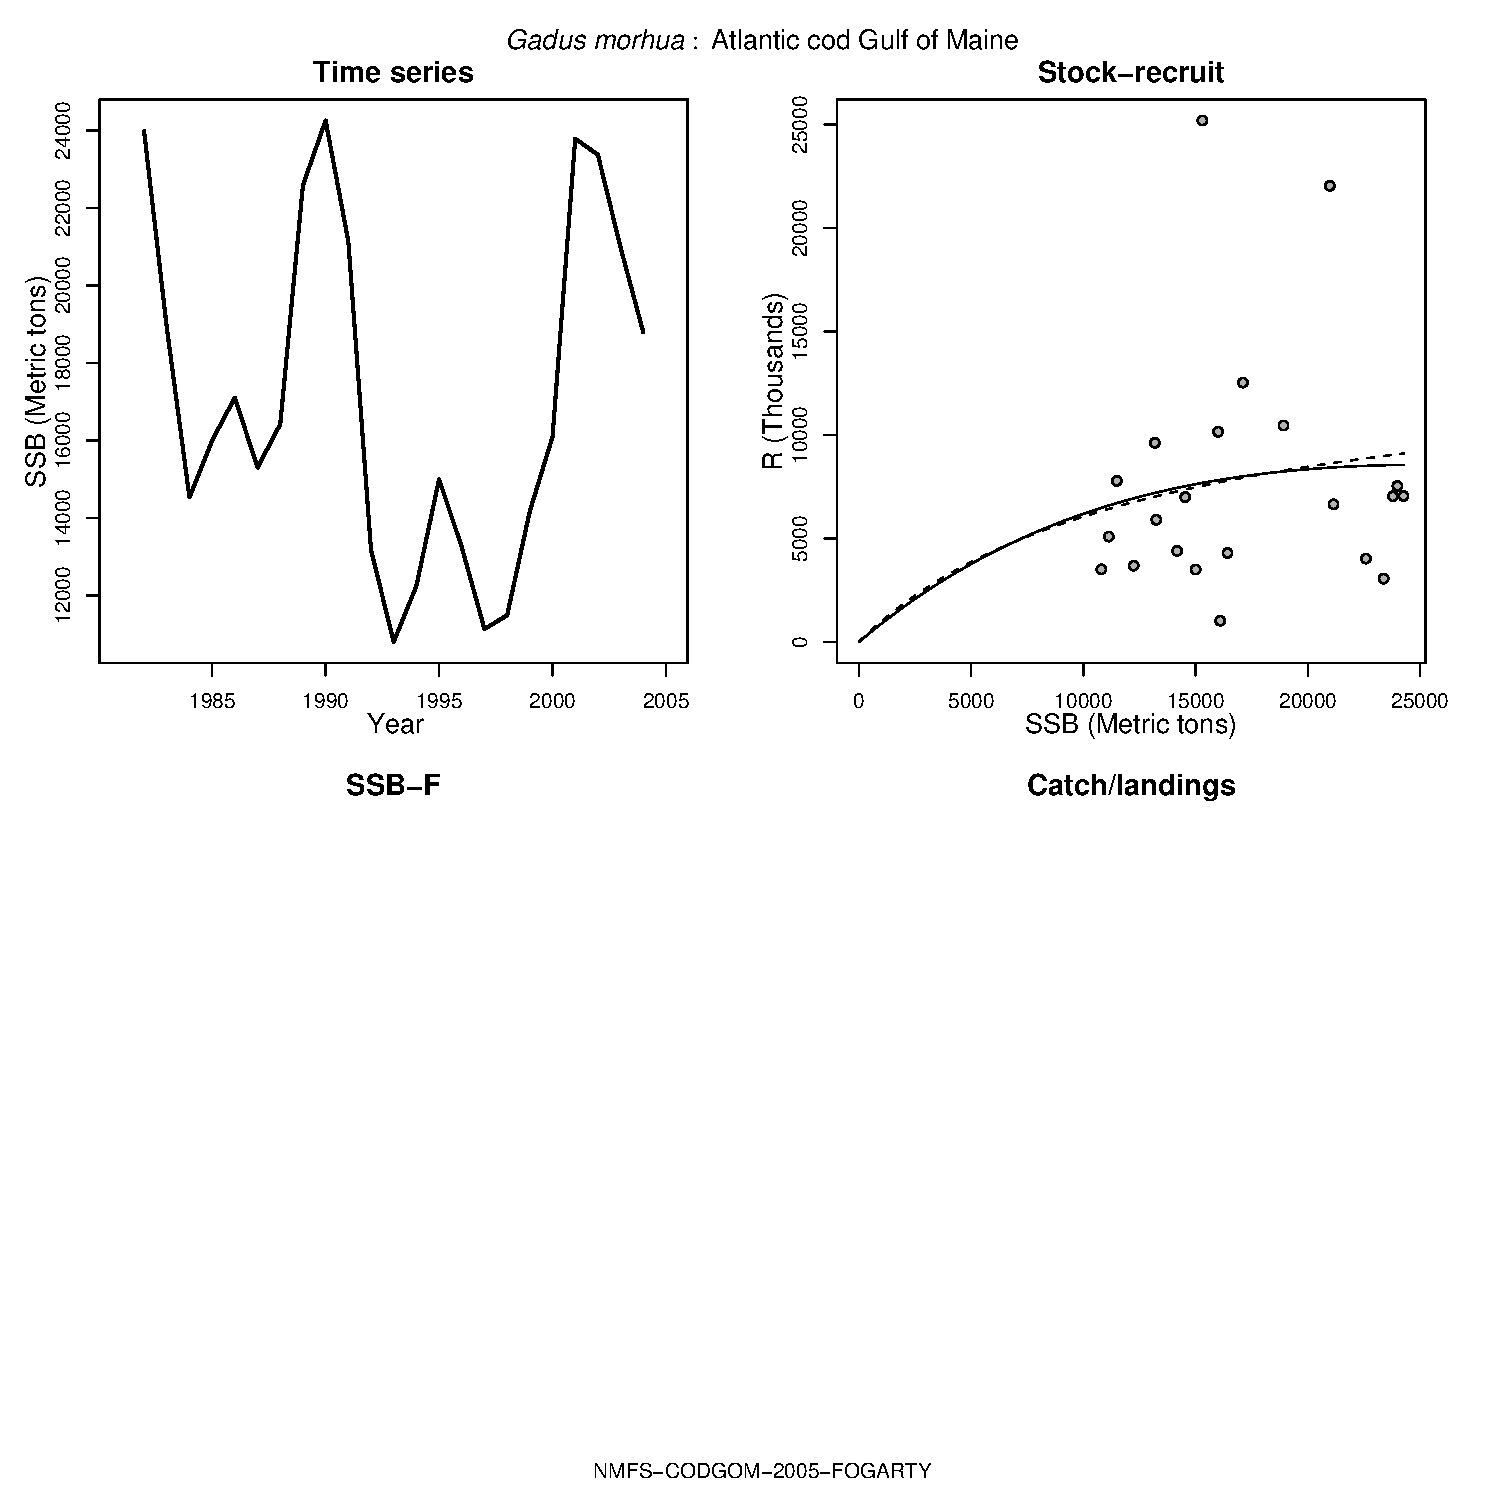
\includegraphics[width=1.2\textwidth]{../R/figures/NMFS-CODGOM-2005-FOGARTY.pdf}
\end{center}

\subsubsection{Gadus morhua - Atlantic cod}\index{Atlantic cod}\index{Gadus morhua}\index{Gadidae!Gadus morhua}
\begin{center}
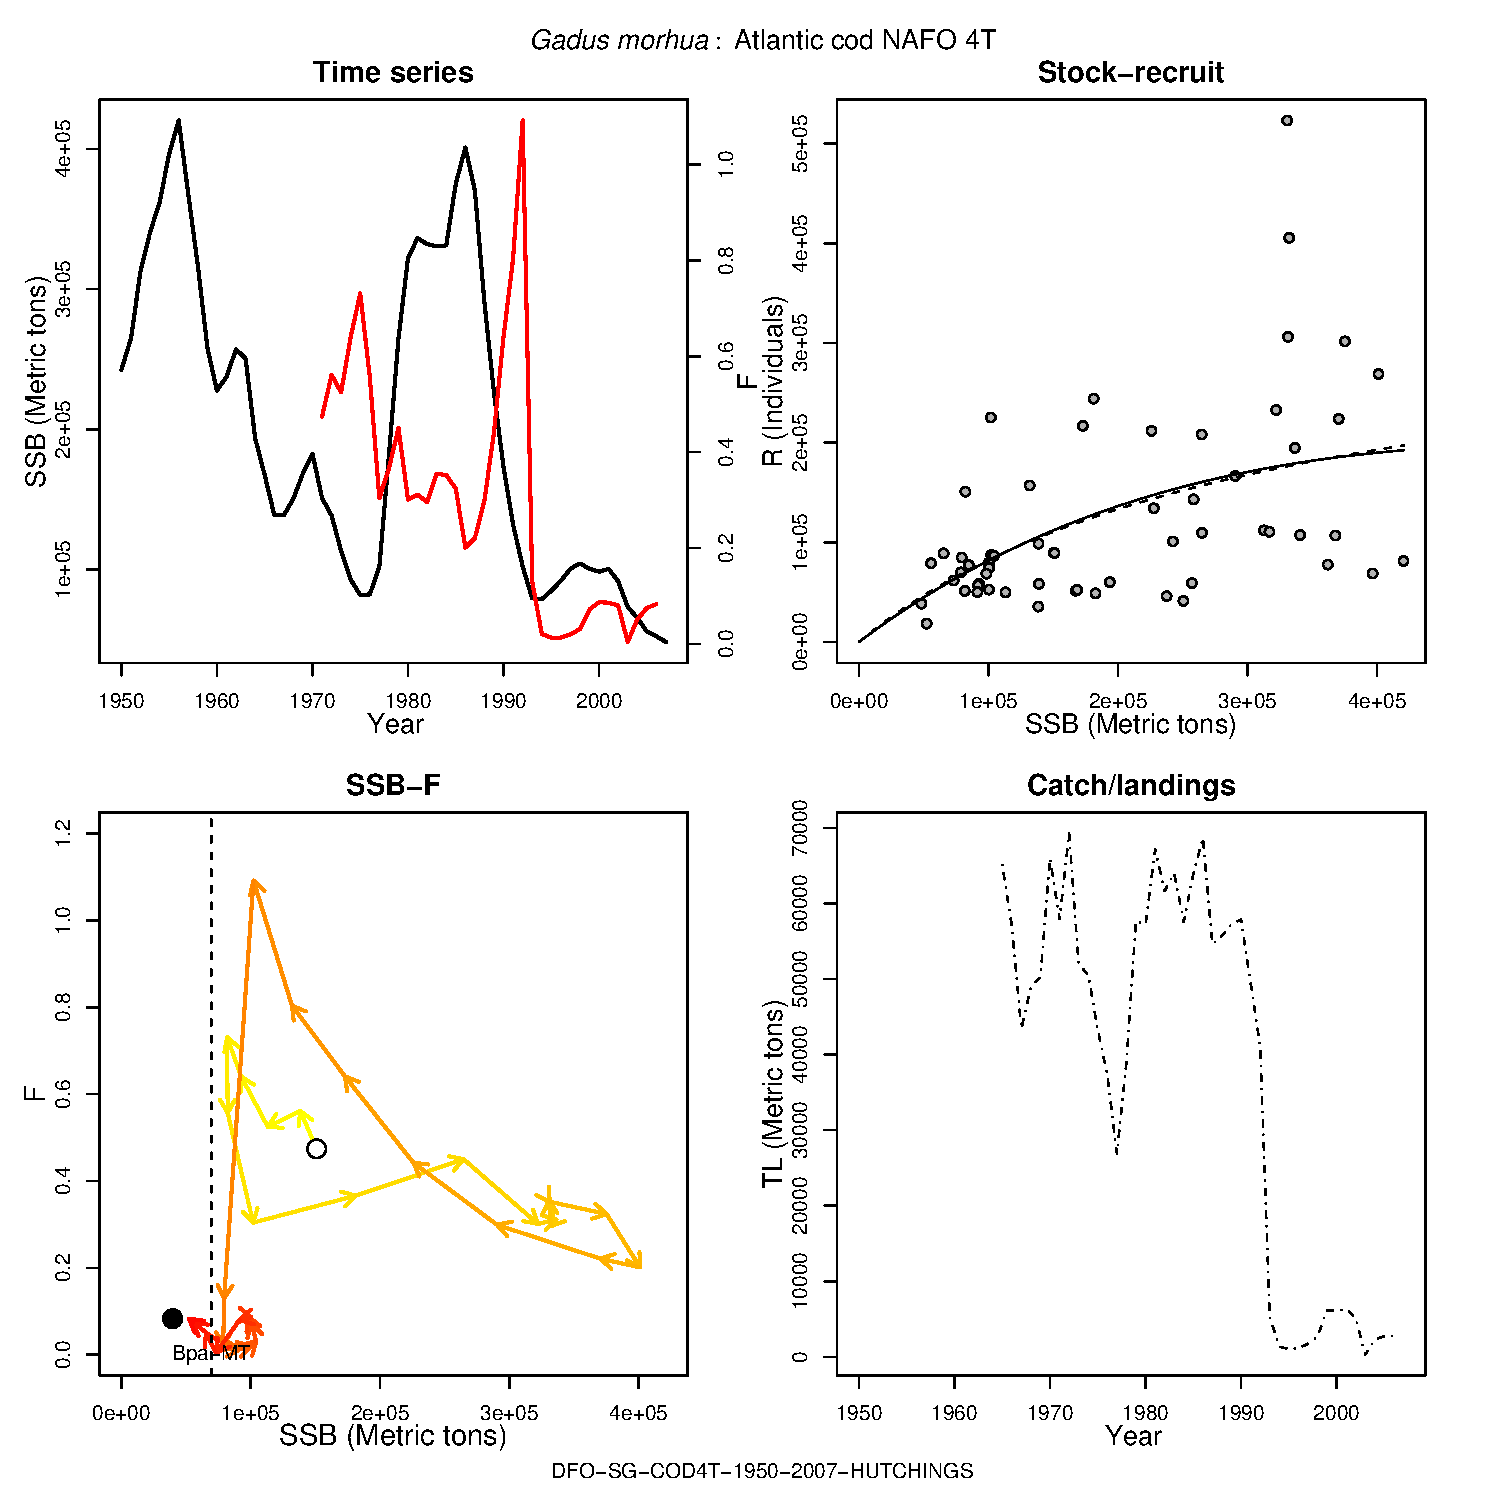
\includegraphics[width=1.2\textwidth]{../R/figures/DFO-SG-COD4T-1950-2007-HUTCHINGS.pdf}
\end{center}

\subsubsection{Gadus morhua - Atlantic cod}\index{Atlantic cod}\index{Gadus morhua}\index{Gadidae!Gadus morhua}
\begin{center}
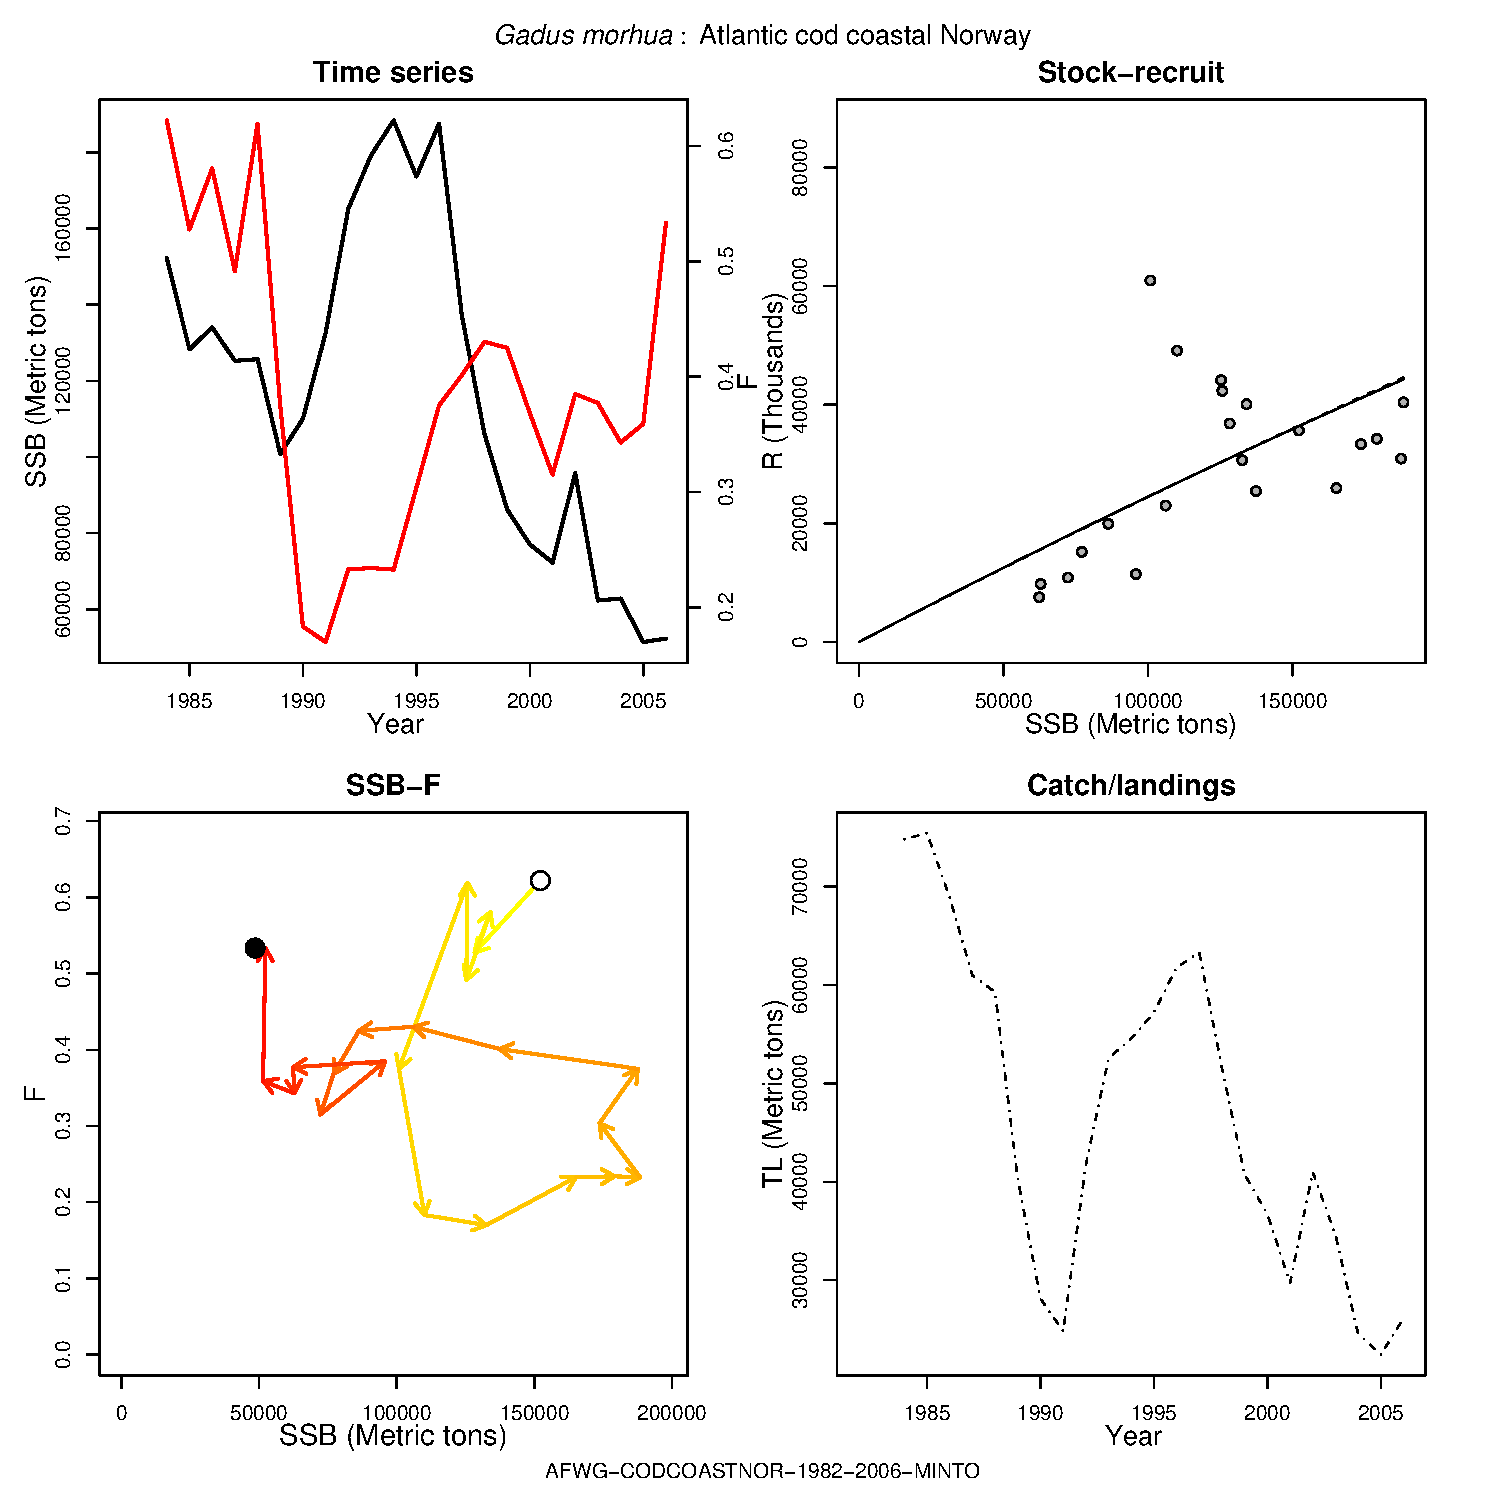
\includegraphics[width=1.2\textwidth]{../R/figures/AFWG-CODCOASTNOR-1982-2006-MINTO.pdf}
\end{center}

\subsubsection{Gadus morhua - Atlantic cod}\index{Atlantic cod}\index{Gadus morhua}\index{Gadidae!Gadus morhua}
\begin{center}
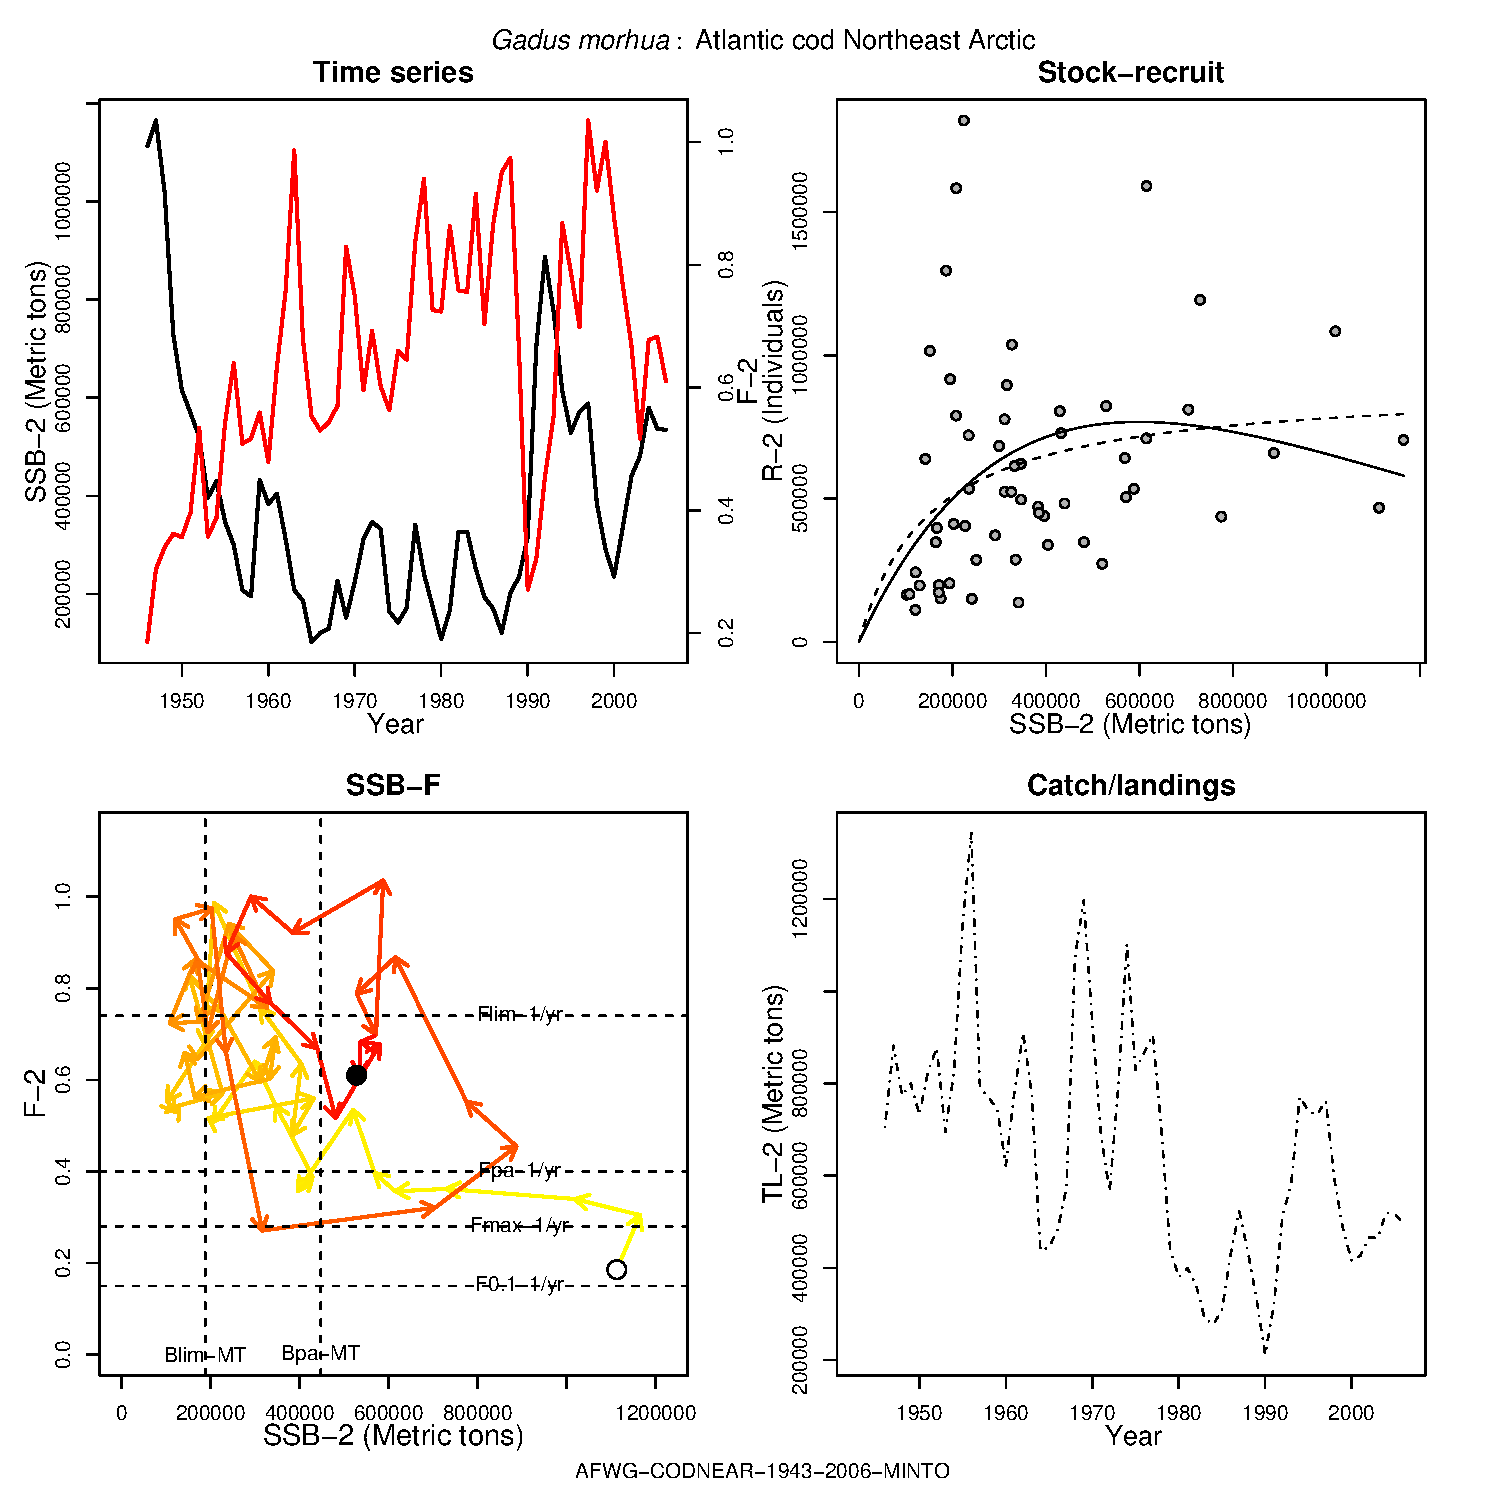
\includegraphics[width=1.2\textwidth]{../R/figures/AFWG-CODNEAR-1943-2006-MINTO.pdf}
\end{center}

\subsubsection{Gadus morhua - Atlantic cod}\index{Atlantic cod}\index{Gadus morhua}\index{Gadidae!Gadus morhua}
\begin{center}
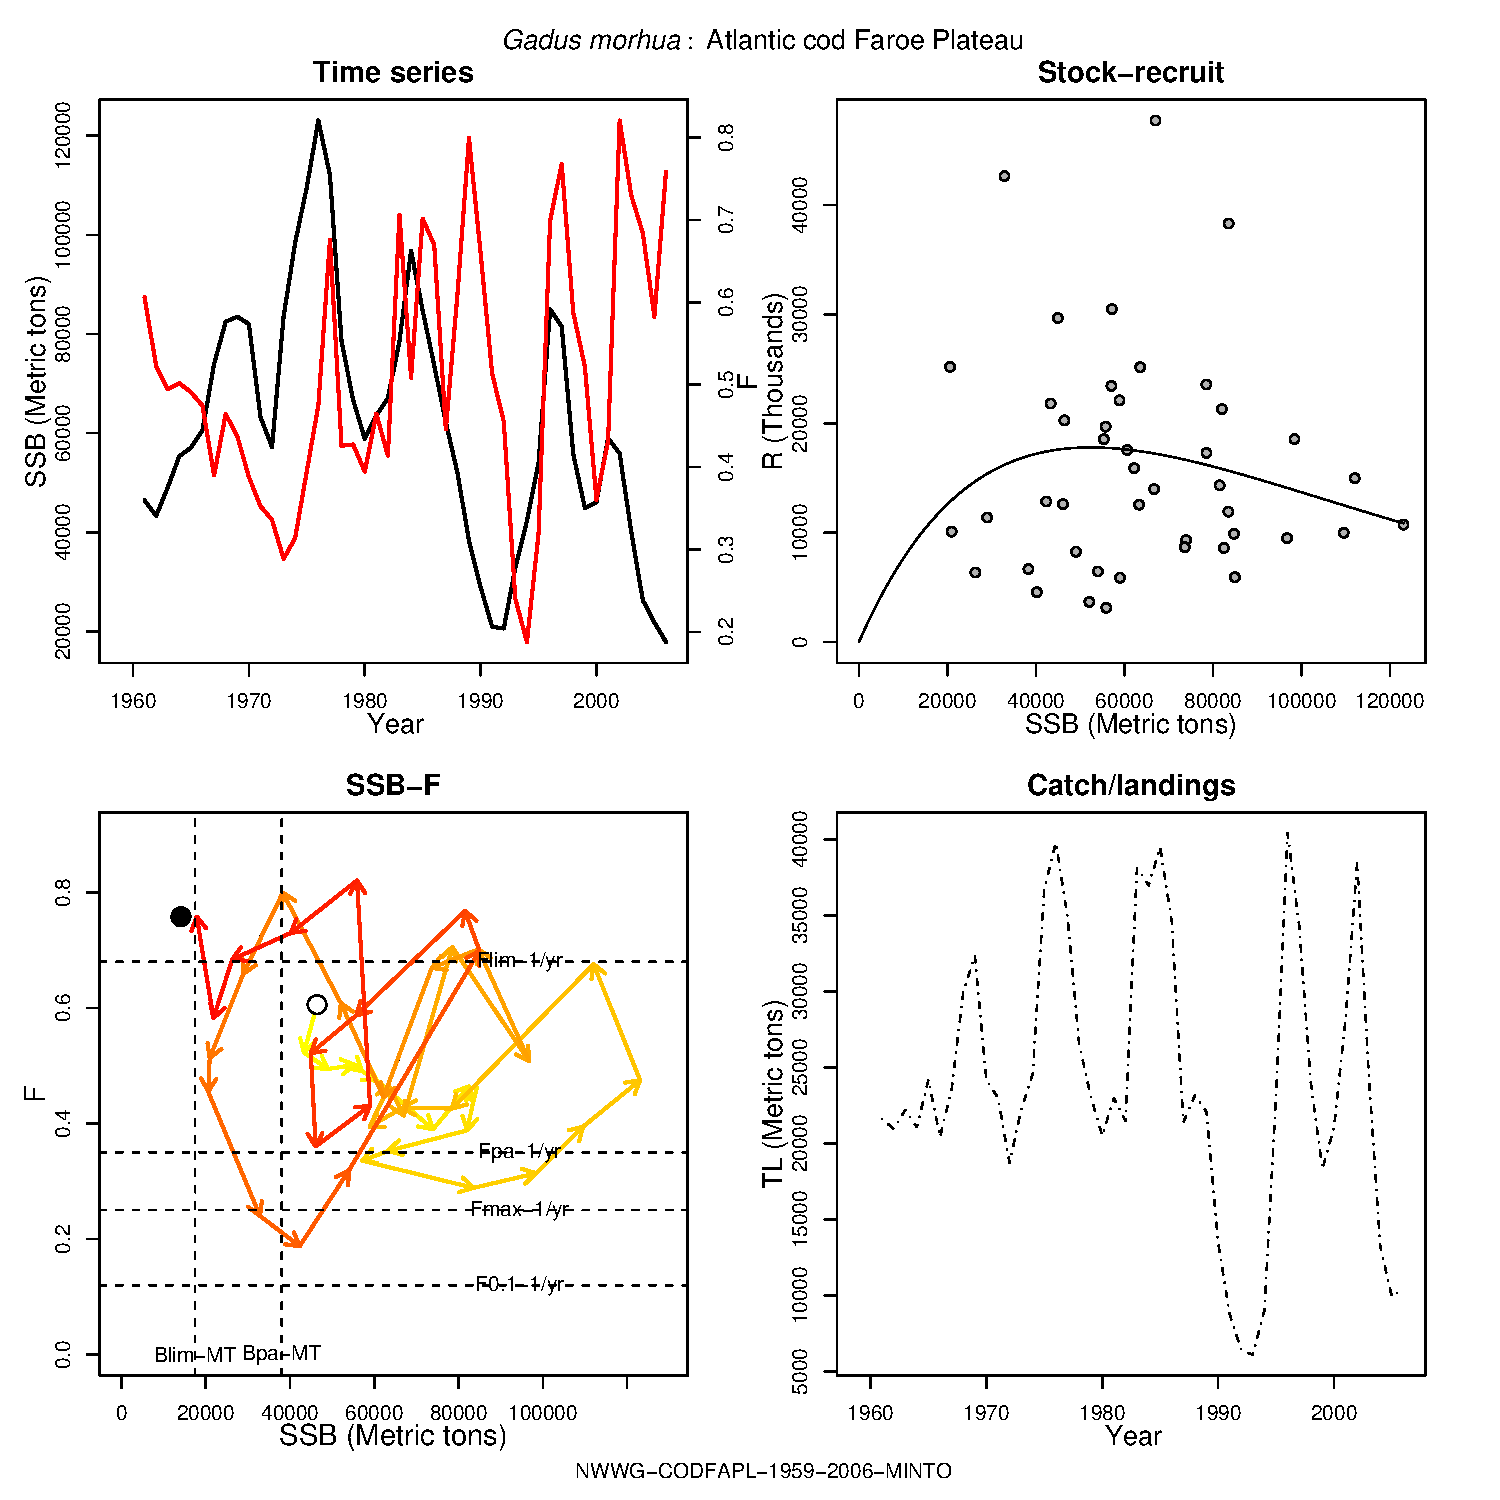
\includegraphics[width=1.2\textwidth]{../R/figures/NWWG-CODFAPL-1959-2006-MINTO.pdf}
\end{center}

\subsubsection{Gadus morhua - Atlantic cod}\index{Atlantic cod}\index{Gadus morhua}\index{Gadidae!Gadus morhua}
\begin{center}
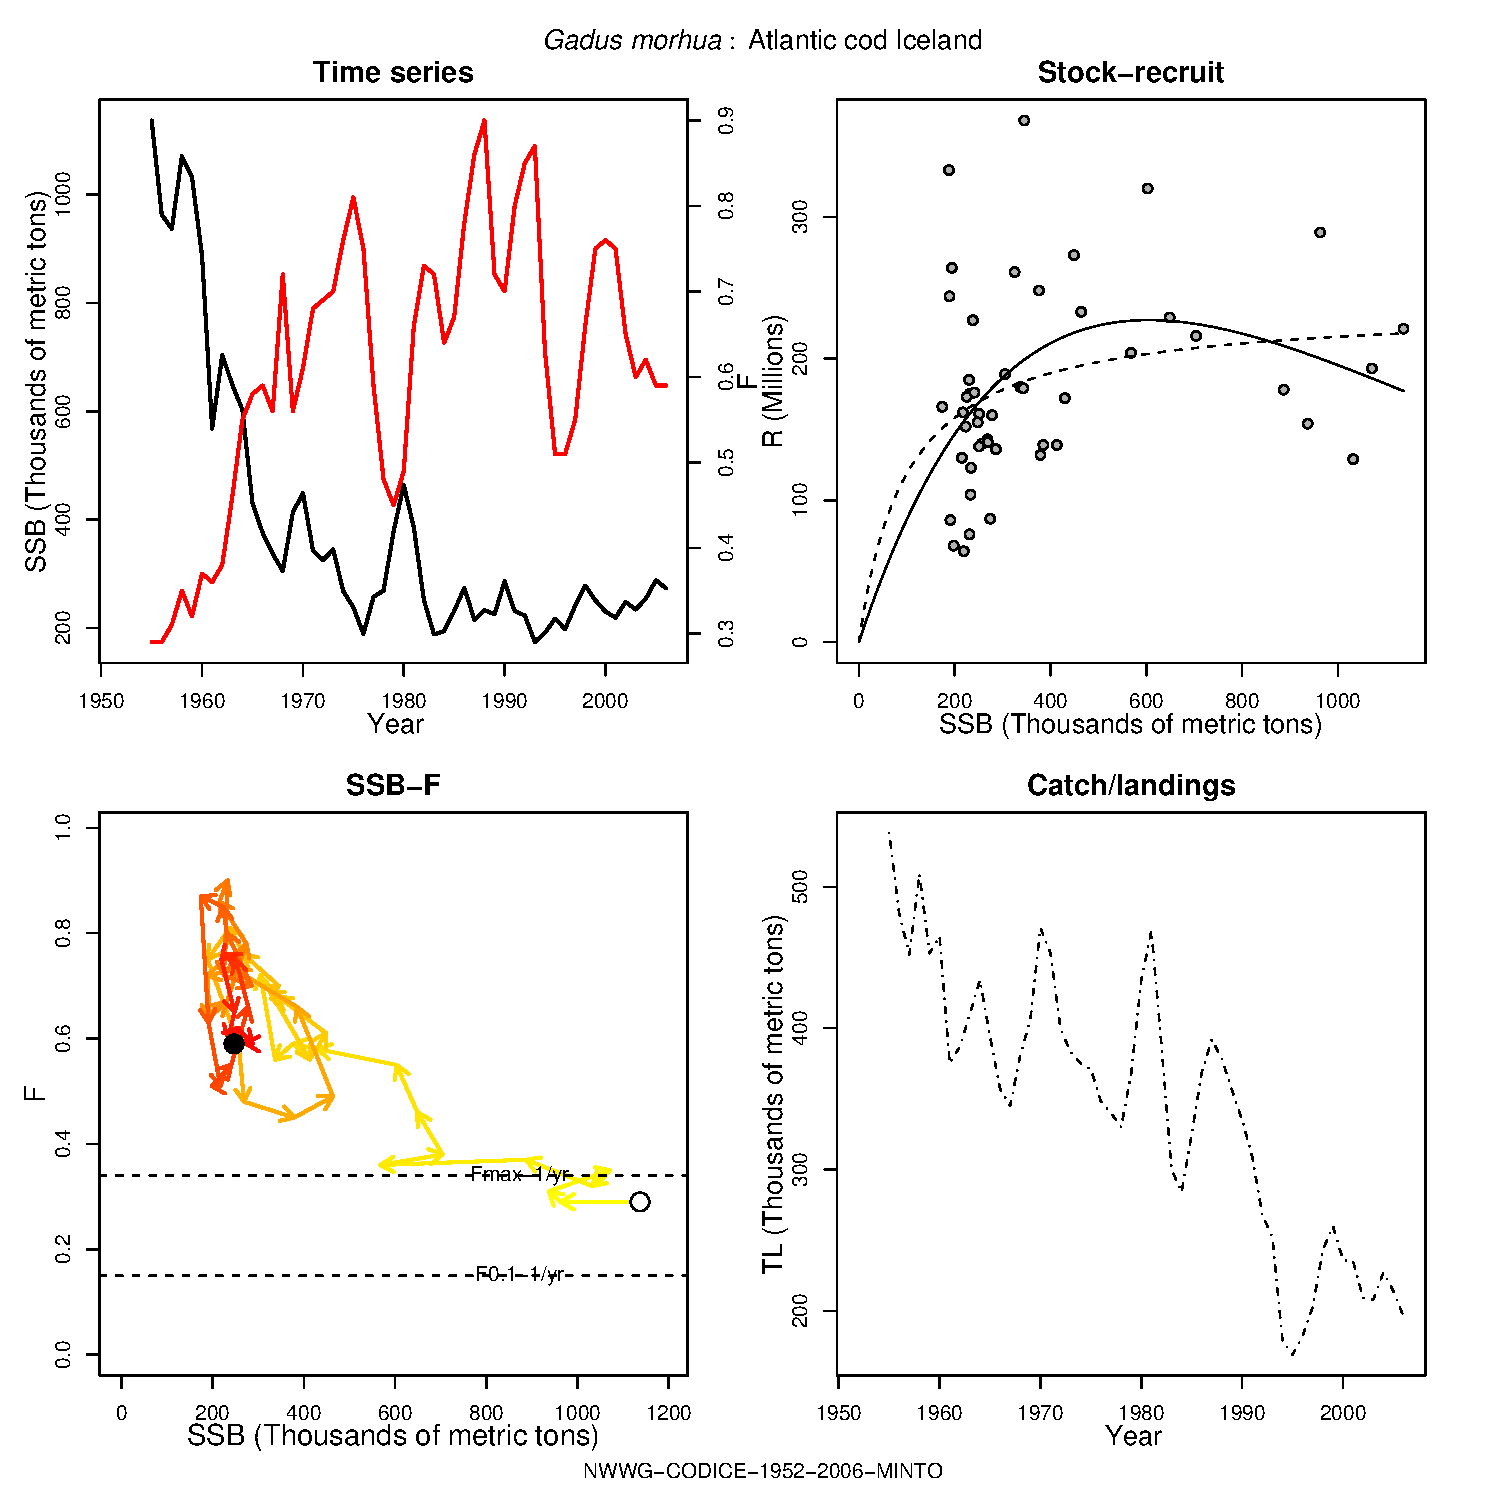
\includegraphics[width=1.2\textwidth]{../R/figures/NWWG-CODICE-1952-2006-MINTO.pdf}
\end{center}

\subsubsection{Gadus morhua - Atlantic cod}\index{Atlantic cod}\index{Gadus morhua}\index{Gadidae!Gadus morhua}
\begin{center}
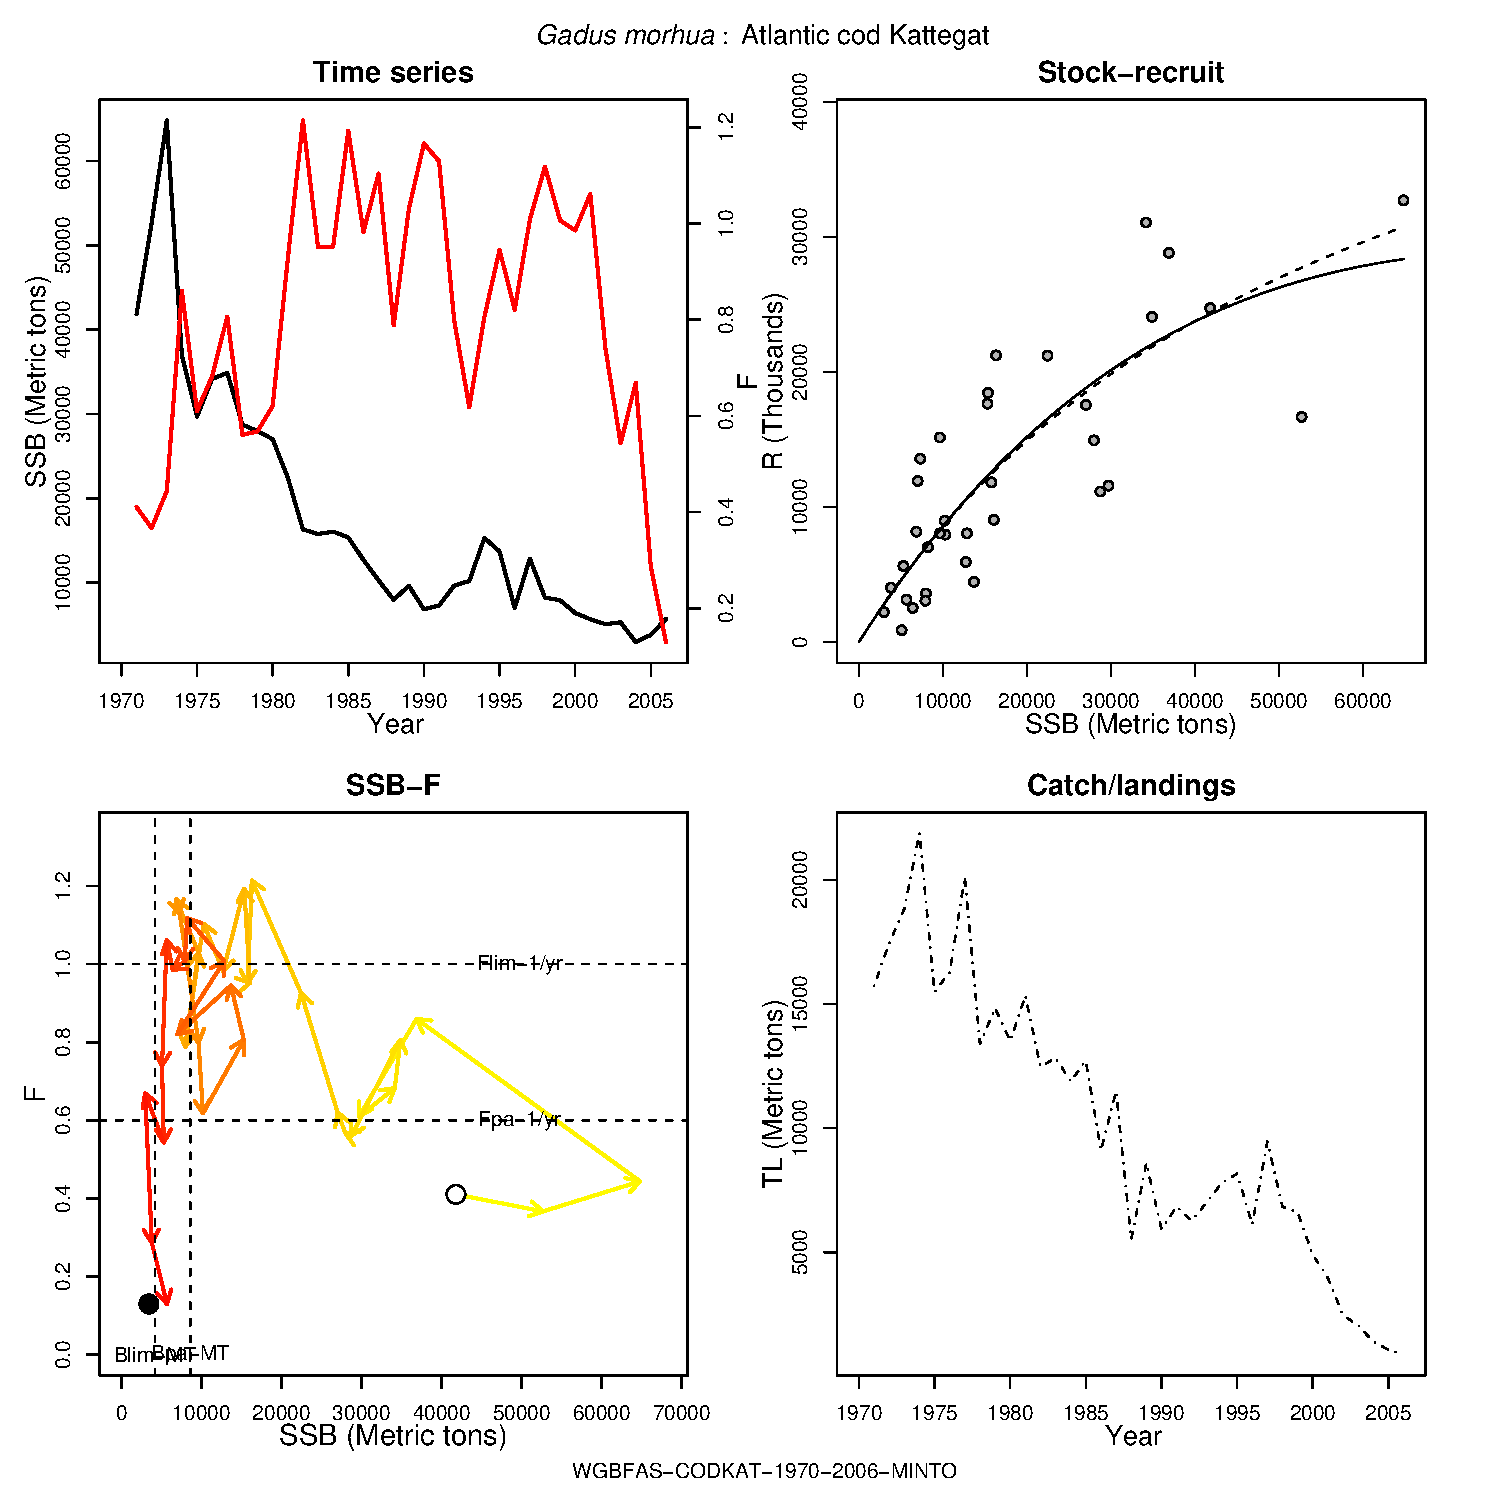
\includegraphics[width=1.2\textwidth]{../R/figures/WGBFAS-CODKAT-1970-2006-MINTO.pdf}
\end{center}

\subsubsection{Gadus morhua - Atlantic cod}\index{Atlantic cod}\index{Gadus morhua}\index{Gadidae!Gadus morhua}
\begin{center}
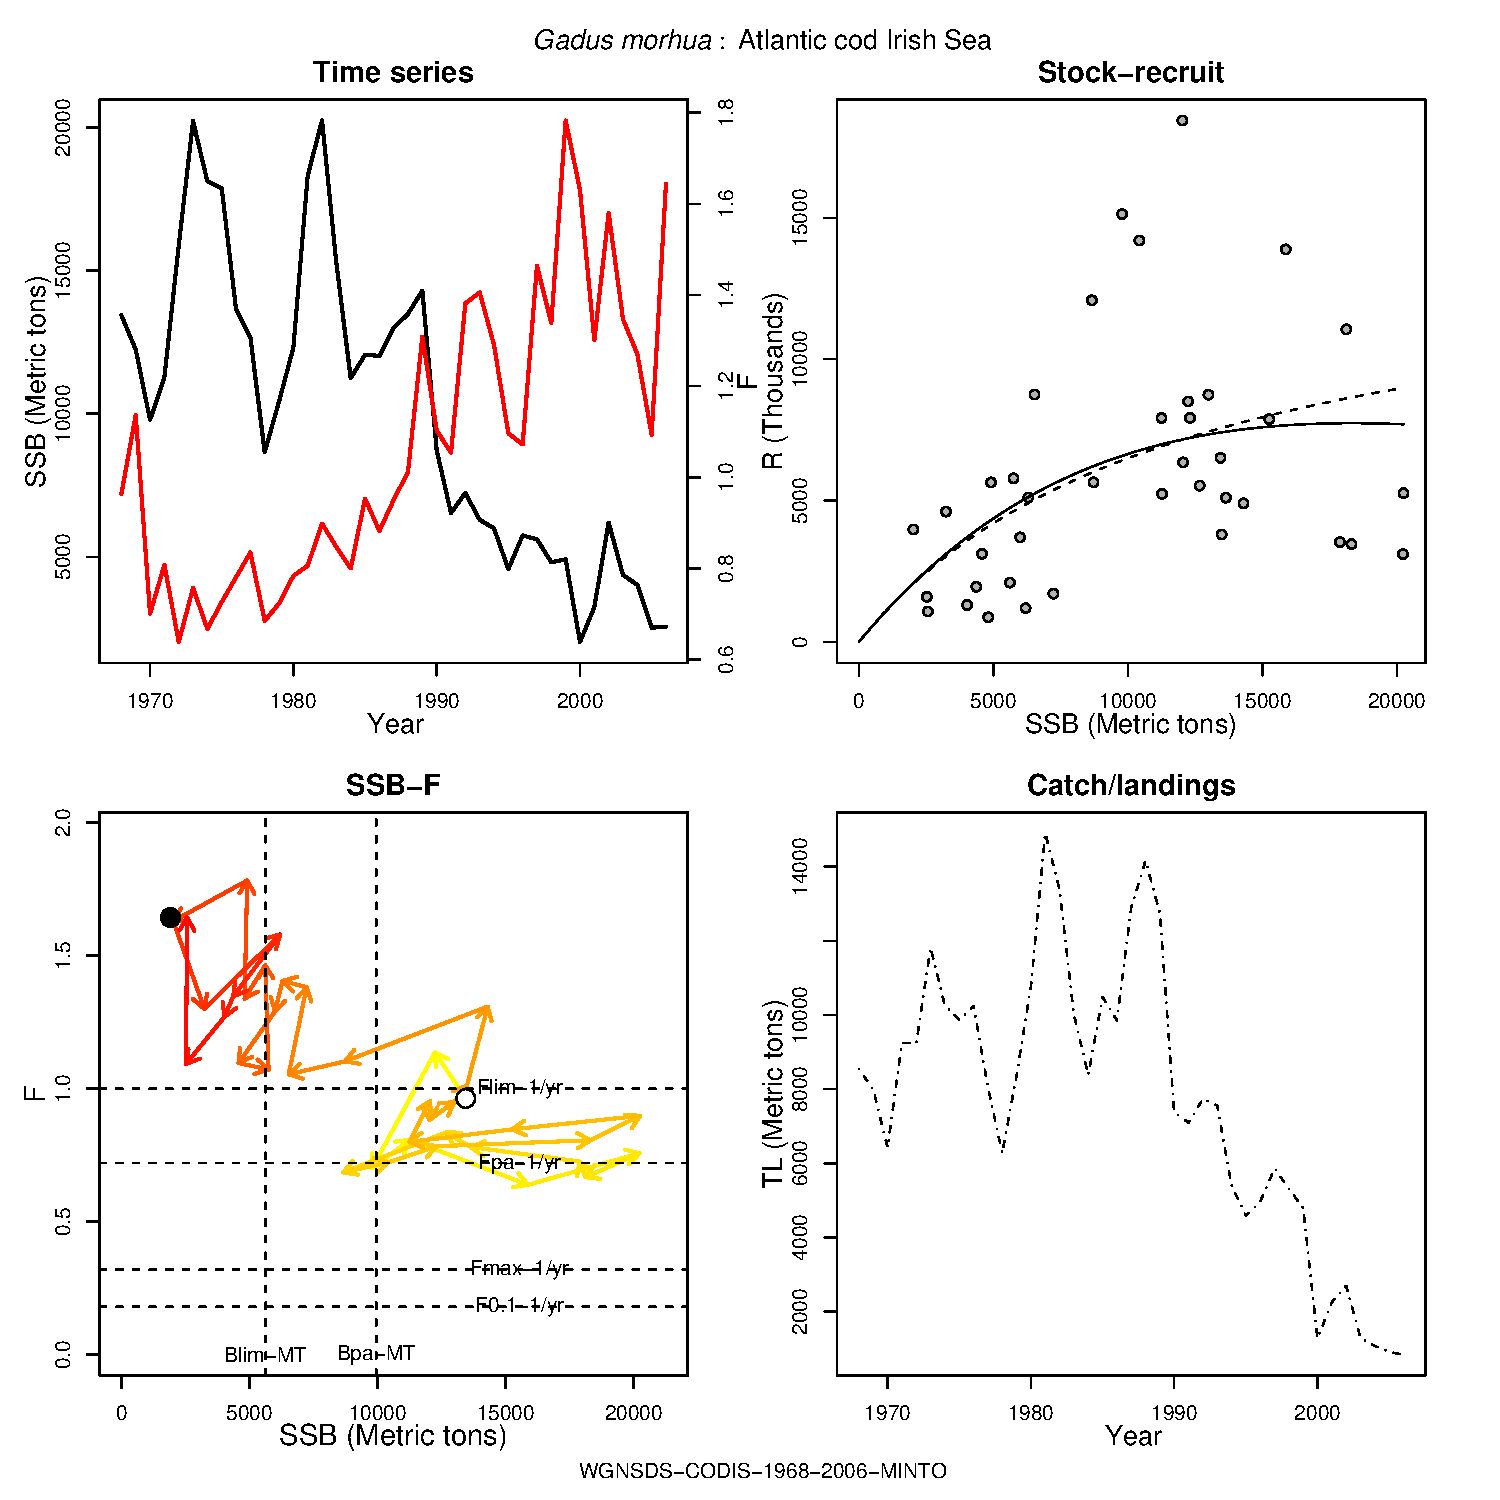
\includegraphics[width=1.2\textwidth]{../R/figures/WGNSDS-CODIS-1968-2006-MINTO.pdf}
\end{center}

\subsubsection{Gadus morhua - Atlantic cod}\index{Atlantic cod}\index{Gadus morhua}\index{Gadidae!Gadus morhua}
\begin{center}
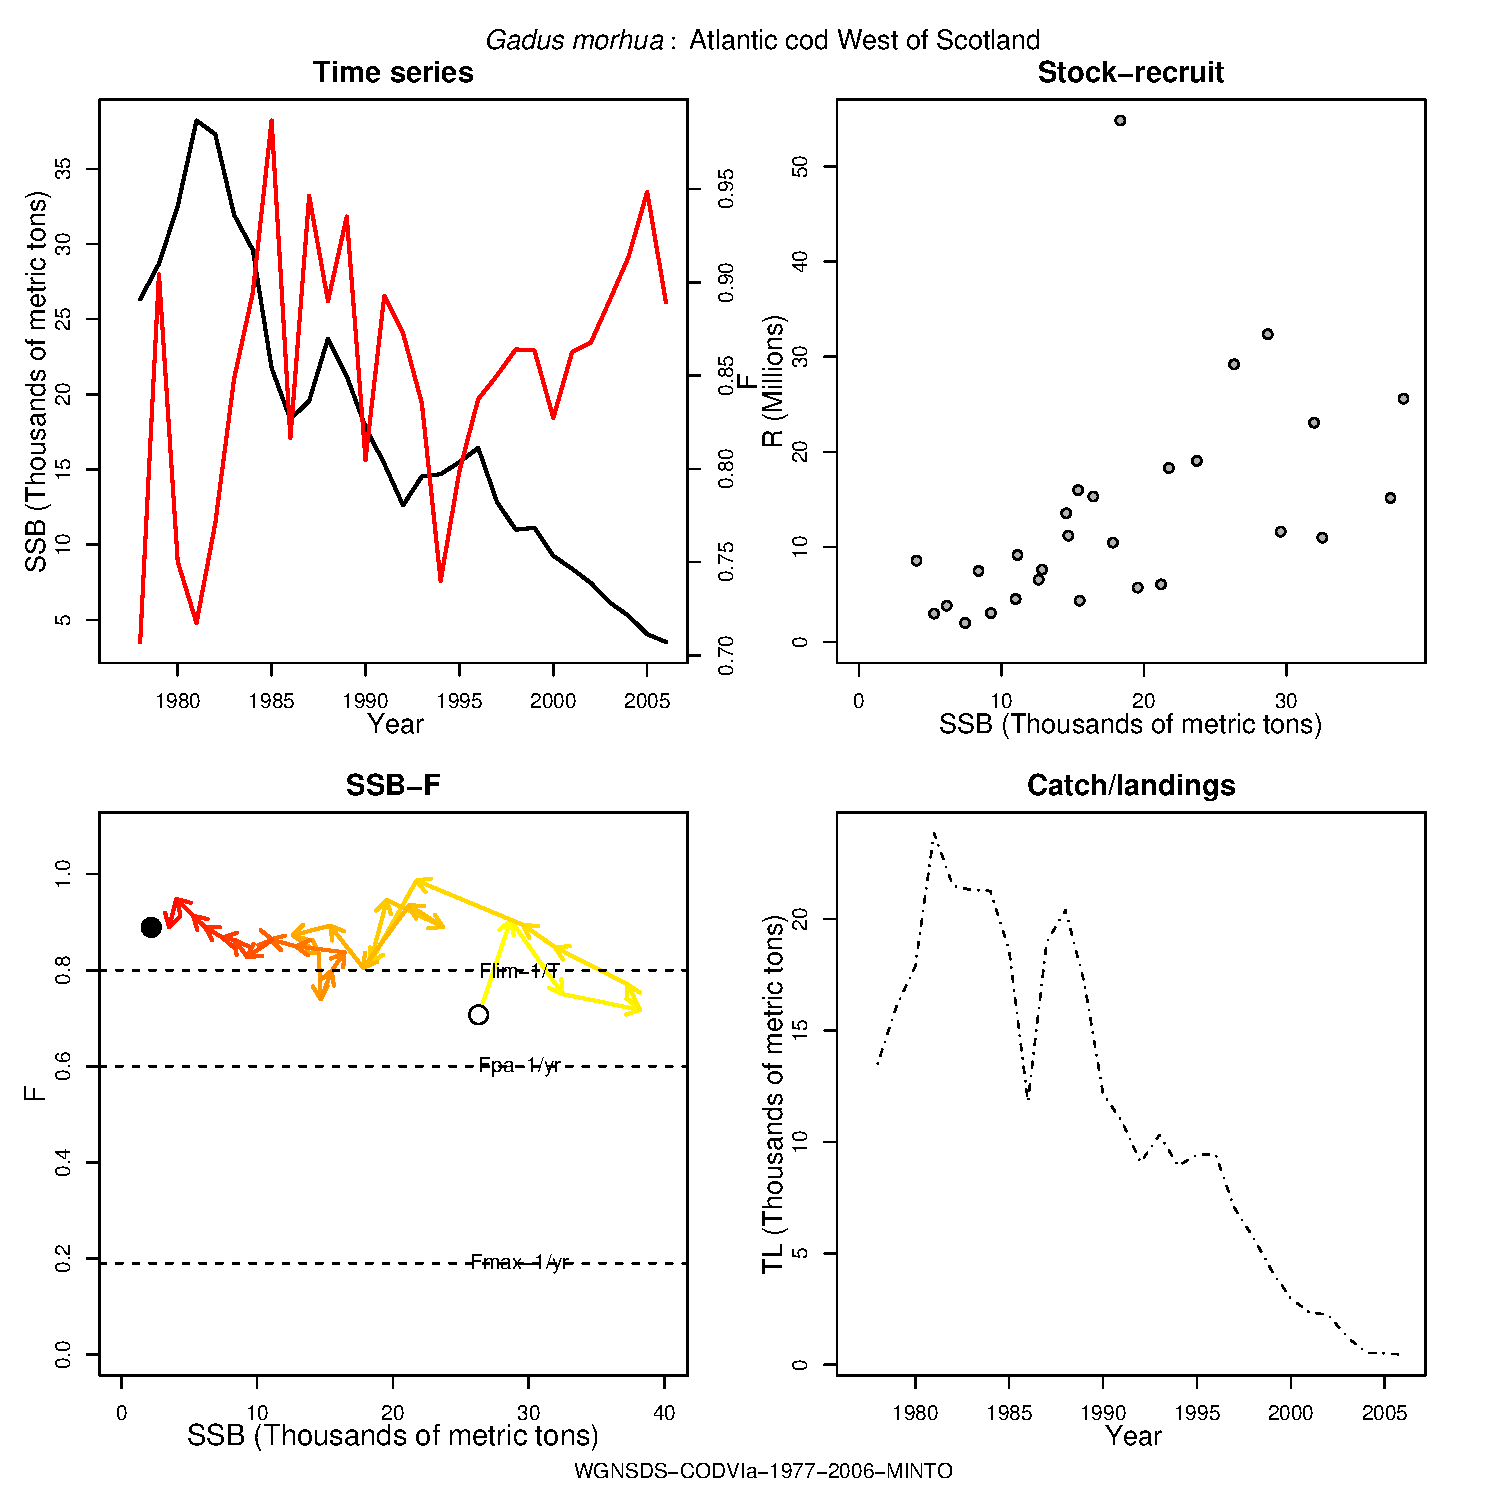
\includegraphics[width=1.2\textwidth]{../R/figures/WGNSDS-CODVIa-1977-2006-MINTO.pdf}
\end{center}

\subsubsection{Gadus morhua - Atlantic cod}\index{Atlantic cod}\index{Gadus morhua}\index{Gadidae!Gadus morhua}
\begin{center}
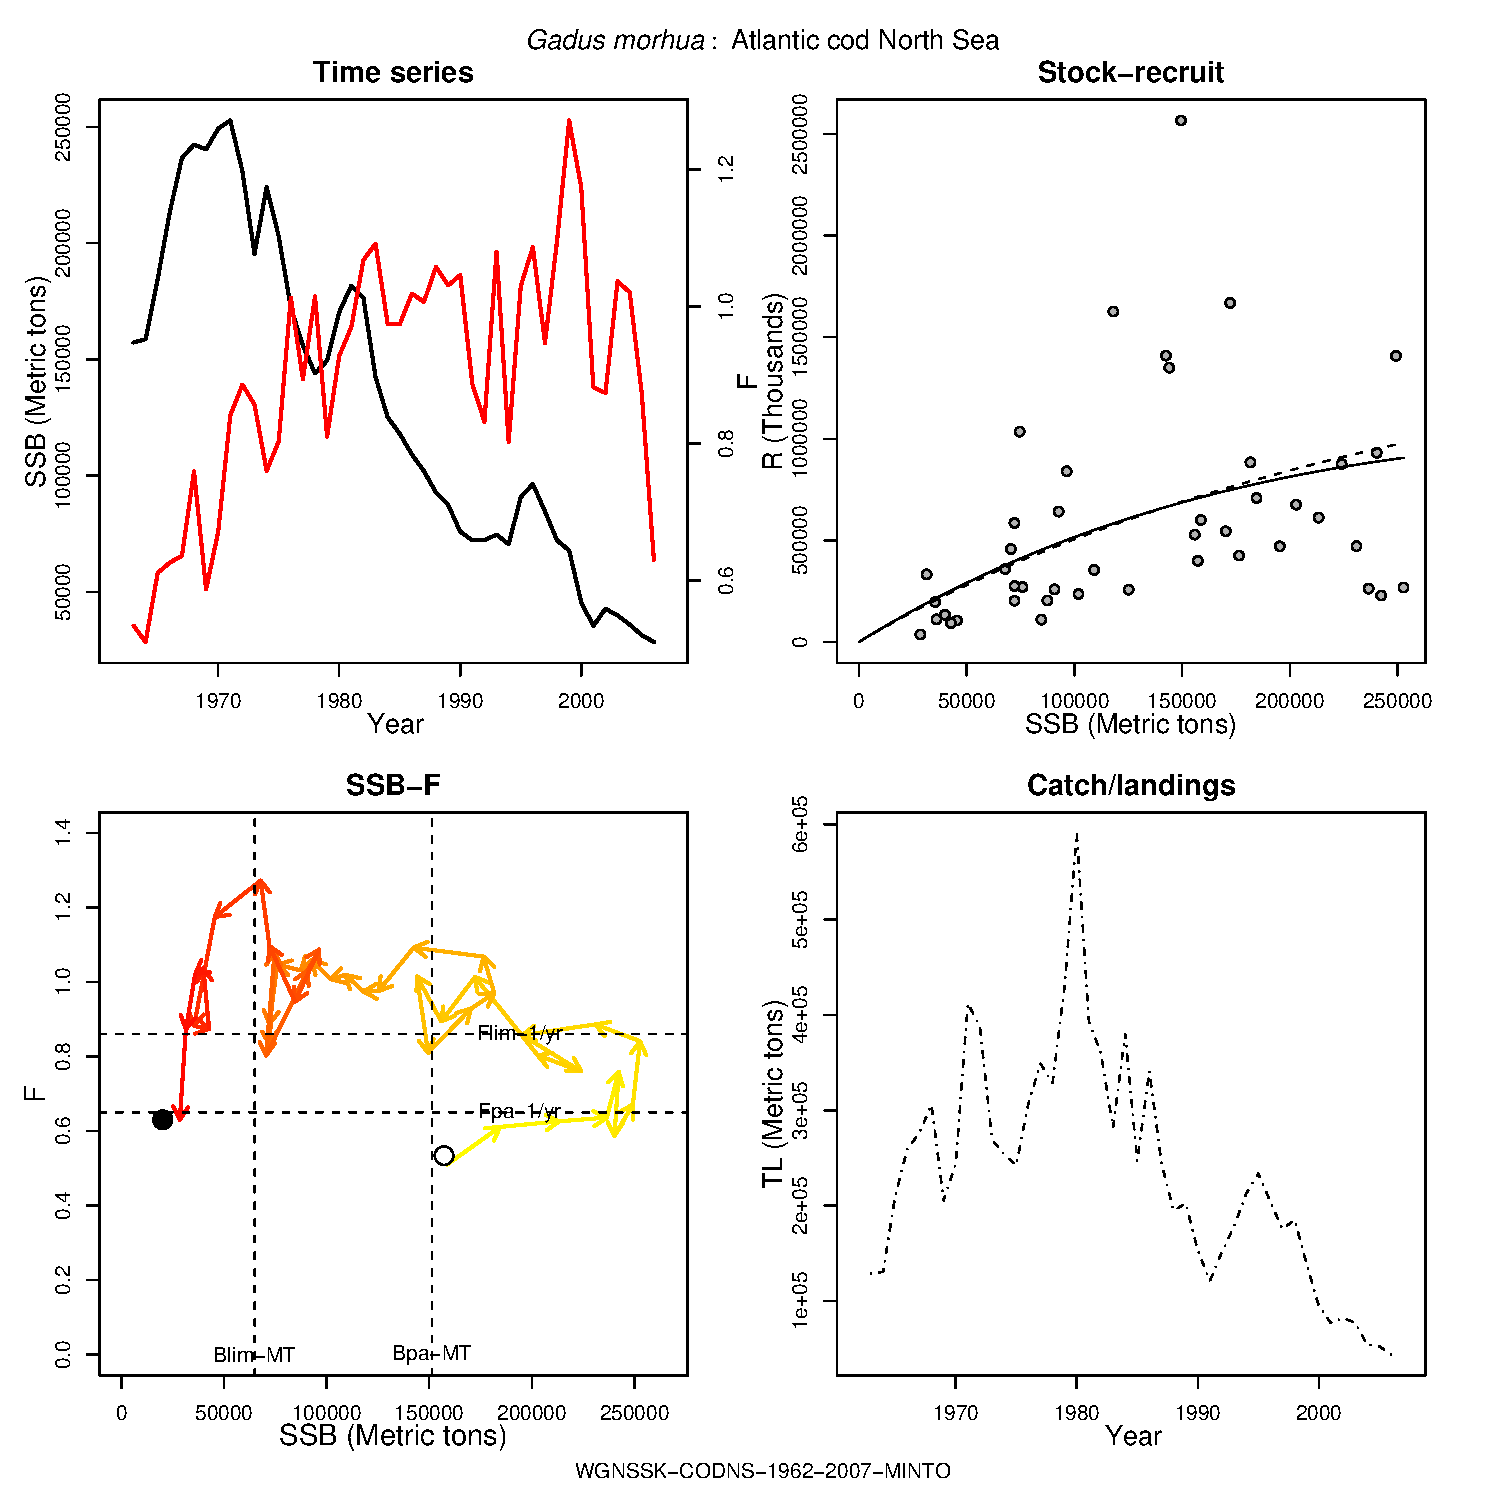
\includegraphics[width=1.2\textwidth]{../R/figures/WGNSSK-CODNS-1962-2007-MINTO.pdf}
\end{center}

\subsubsection{Gadus morhua - Atlantic cod}\index{Atlantic cod}\index{Gadus morhua}\index{Gadidae!Gadus morhua}
\begin{center}
\includegraphics[width=1.2\textwidth]{../R/figures/PHONYassessorid-COD1-1952-1992-MYERS.pdf}
\end{center}

\subsubsection{Gadus morhua - Atlantic cod}\index{Atlantic cod}\index{Gadus morhua}\index{Gadidae!Gadus morhua}
\begin{center}
\includegraphics[width=1.2\textwidth]{../R/figures/PHONYassessorid-COD2J3KL-1850-2000-MYERS.pdf}
\end{center}

\subsubsection{Gadus morhua - Atlantic cod}\index{Atlantic cod}\index{Gadus morhua}\index{Gadidae!Gadus morhua}
\begin{center}
\includegraphics[width=1.2\textwidth]{../R/figures/PHONYassessorid-COD3NO-1953-2002-MYERS.pdf}
\end{center}

\subsubsection{Gadus morhua - Atlantic cod}\index{Atlantic cod}\index{Gadus morhua}\index{Gadidae!Gadus morhua}
\begin{center}
\includegraphics[width=1.2\textwidth]{../R/figures/PHONYassessorid-COD4VsW-1957-1993-MYERS.pdf}
\end{center}

\subsubsection{Gadus morhua - Atlantic cod}\index{Atlantic cod}\index{Gadus morhua}\index{Gadidae!Gadus morhua}
\begin{center}
\includegraphics[width=1.2\textwidth]{../R/figures/PHONYassessorid-COD4X-1947-2001-MYERS.pdf}
\end{center}

\subsubsection{Gadus morhua - Atlantic cod}\index{Atlantic cod}\index{Gadus morhua}\index{Gadidae!Gadus morhua}
\begin{center}
\includegraphics[width=1.2\textwidth]{../R/figures/PHONYassessorid-COD5Z-1977-1998-MYERS.pdf}
\end{center}

\subsubsection{Gadus morhua - Atlantic cod}\index{Atlantic cod}\index{Gadus morhua}\index{Gadidae!Gadus morhua}
\begin{center}
\includegraphics[width=1.2\textwidth]{../R/figures/PHONYassessorid-CODBA2532-1964-2003-MYERS.pdf}
\end{center}

\subsubsection{Gadus morhua - Atlantic cod}\index{Atlantic cod}\index{Gadus morhua}\index{Gadidae!Gadus morhua}
\begin{center}
\includegraphics[width=1.2\textwidth]{../R/figures/PHONYassessorid-CODCOASTNOR-1982-2000-MYERS.pdf}
\end{center}

\subsubsection{Gadus morhua - Atlantic cod}\index{Atlantic cod}\index{Gadus morhua}\index{Gadidae!Gadus morhua}
\begin{center}
\includegraphics[width=1.2\textwidth]{../R/figures/PHONYassessorid-CODFAPL-1924-2000-MYERS.pdf}
\end{center}

\subsubsection{Gadus morhua - Atlantic cod}\index{Atlantic cod}\index{Gadus morhua}\index{Gadidae!Gadus morhua}
\begin{center}
\includegraphics[width=1.2\textwidth]{../R/figures/PHONYassessorid-CODICE-1905-2000-MYERS.pdf}
\end{center}

\subsubsection{Gadus morhua - Atlantic cod}\index{Atlantic cod}\index{Gadus morhua}\index{Gadidae!Gadus morhua}
\begin{center}
\includegraphics[width=1.2\textwidth]{../R/figures/PHONYassessorid-CODKAT-1970-2000-MYERS.pdf}
\end{center}

\subsubsection{Gadus morhua - Atlantic cod}\index{Atlantic cod}\index{Gadus morhua}\index{Gadidae!Gadus morhua}
\begin{center}
\includegraphics[width=1.2\textwidth]{../R/figures/PHONYassessorid-CODNEAR-1930-1991-MYERS.pdf}
\end{center}

\subsubsection{Gadus morhua - Atlantic cod}\index{Atlantic cod}\index{Gadus morhua}\index{Gadidae!Gadus morhua}
\begin{center}
\includegraphics[width=1.2\textwidth]{../R/figures/PHONYassessorid-CODNS-1930-2002-MYERS.pdf}
\end{center}

\subsubsection{Gadus morhua - Atlantic cod}\index{Atlantic cod}\index{Gadus morhua}\index{Gadidae!Gadus morhua}
\begin{center}
\includegraphics[width=1.2\textwidth]{../R/figures/PHONYassessorid-CODVIa-1965-2000-MYERS.pdf}
\end{center}

\subsubsection{Gadus morhua - Atlantic cod}\index{Atlantic cod}\index{Gadus morhua}\index{Gadidae!Gadus morhua}
\begin{center}
\includegraphics[width=1.2\textwidth]{../R/figures/DFO-COD5Zjm-1978-2003-PREFONTAINE.pdf}
\end{center}

\subsubsection{Gadus morhua - Atlantic cod}\index{Atlantic cod}\index{Gadus morhua}\index{Gadidae!Gadus morhua}
\begin{center}
\includegraphics[width=1.2\textwidth]{../R/figures/DFO-NFLD-COD2J3KLIS-1959-2006-PREFONTAINE.pdf}
\end{center}

\subsubsection{Gadus morhua - Atlantic cod}\index{Atlantic cod}\index{Gadus morhua}\index{Gadidae!Gadus morhua}
\begin{center}
\includegraphics[width=1.2\textwidth]{../R/figures/NAFO-SC-COD3NO-1953-2007-PREFONTAINE.pdf}
\end{center}

\subsubsection{Melanogrammus aeglefinus - Haddock}\index{Haddock}\index{Melanogrammus aeglefinus}\index{Gadidae!Melanogrammus aeglefinus}
\begin{center}
\includegraphics[width=1.2\textwidth]{../R/figures/NMFS-HADGB-2005-FOGARTY.pdf}
\end{center}

\subsubsection{Melanogrammus aeglefinus - Haddock}\index{Haddock}\index{Melanogrammus aeglefinus}\index{Gadidae!Melanogrammus aeglefinus}
\begin{center}
\includegraphics[width=1.2\textwidth]{../R/figures/AFWG-HADNEAR-1947-2006-MINTO.pdf}
\end{center}

\subsubsection{Melanogrammus aeglefinus - Haddock}\index{Haddock}\index{Melanogrammus aeglefinus}\index{Gadidae!Melanogrammus aeglefinus}
\begin{center}
\includegraphics[width=1.2\textwidth]{../R/figures/NWWG-HADFAPL-1955-2007-MINTO.pdf}
\end{center}

\subsubsection{Melanogrammus aeglefinus - Haddock}\index{Haddock}\index{Melanogrammus aeglefinus}\index{Gadidae!Melanogrammus aeglefinus}
\begin{center}
\includegraphics[width=1.2\textwidth]{../R/figures/NWWG-HADICE-1977-2007-MINTO.pdf}
\end{center}

\subsubsection{Melanogrammus aeglefinus - Haddock}\index{Haddock}\index{Melanogrammus aeglefinus}\index{Gadidae!Melanogrammus aeglefinus}
\begin{center}
\includegraphics[width=1.2\textwidth]{../R/figures/WGNSDS-HADIS-1991-2006-MINTO.pdf}
\end{center}

\subsubsection{Melanogrammus aeglefinus - Haddock}\index{Haddock}\index{Melanogrammus aeglefinus}\index{Gadidae!Melanogrammus aeglefinus}
\begin{center}
\includegraphics[width=1.2\textwidth]{../R/figures/WGNSDS-HADVIa-1977-2006-MINTO.pdf}
\end{center}

\subsubsection{Melanogrammus aeglefinus - Haddock}\index{Haddock}\index{Melanogrammus aeglefinus}\index{Gadidae!Melanogrammus aeglefinus}
\begin{center}
\includegraphics[width=1.2\textwidth]{../R/figures/WGNSSK-HADNS-IIIa-1963-2006-MINTO.pdf}
\end{center}

\subsubsection{Melanogrammus aeglefinus - Haddock}\index{Haddock}\index{Melanogrammus aeglefinus}\index{Gadidae!Melanogrammus aeglefinus}
\begin{center}
\includegraphics[width=1.2\textwidth]{../R/figures/PHONYassessorid-HADFAPL-1959-2000-MYERS.pdf}
\end{center}

\subsubsection{Melanogrammus aeglefinus - Haddock}\index{Haddock}\index{Melanogrammus aeglefinus}\index{Gadidae!Melanogrammus aeglefinus}
\begin{center}
\includegraphics[width=1.2\textwidth]{../R/figures/PHONYassessorid-HADICE-1950-1990-MYERS.pdf}
\end{center}

\subsubsection{Melanogrammus aeglefinus - Haddock}\index{Haddock}\index{Melanogrammus aeglefinus}\index{Gadidae!Melanogrammus aeglefinus}
\begin{center}
\includegraphics[width=1.2\textwidth]{../R/figures/PHONYassessorid-HADIS-1993-2000-MYERS.pdf}
\end{center}

\subsubsection{Melanogrammus aeglefinus - Haddock}\index{Haddock}\index{Melanogrammus aeglefinus}\index{Gadidae!Melanogrammus aeglefinus}
\begin{center}
\includegraphics[width=1.2\textwidth]{../R/figures/PHONYassessorid-HADNEAR-1947-2004-MYERS.pdf}
\end{center}

\subsubsection{Melanogrammus aeglefinus - Haddock}\index{Haddock}\index{Melanogrammus aeglefinus}\index{Gadidae!Melanogrammus aeglefinus}
\begin{center}
\includegraphics[width=1.2\textwidth]{../R/figures/PHONYassessorid-HADVIa-1965-1993-MYERS.pdf}
\end{center}

\subsubsection{Melanogrammus aeglefinus - Haddock}\index{Haddock}\index{Melanogrammus aeglefinus}\index{Gadidae!Melanogrammus aeglefinus}
\begin{center}
\includegraphics[width=1.2\textwidth]{../R/figures/DFO-HAD4X5Y-1960-2003-PREFONTAINE.pdf}
\end{center}

\subsubsection{Melanogrammus aeglefinus - Haddock}\index{Haddock}\index{Melanogrammus aeglefinus}\index{Gadidae!Melanogrammus aeglefinus}
\begin{center}
\includegraphics[width=1.2\textwidth]{../R/figures/DFO-HAD5Zejm-1969-2003-PREFONTAINE.pdf}
\end{center}

\subsubsection{Merlangius merlangus - Whiting}\index{Whiting}\index{Merlangius merlangus}\index{Gadidae!Merlangius merlangus}
\begin{center}
\includegraphics[width=1.2\textwidth]{../R/figures/WGNSDS-WHITVIa-1984-2007-MINTO.pdf}
\end{center}

\subsubsection{Merlangius merlangus - Whiting}\index{Whiting}\index{Merlangius merlangus}\index{Gadidae!Merlangius merlangus}
\begin{center}
\includegraphics[width=1.2\textwidth]{../R/figures/WGNSSK-WHITNS-VIId-IIIa-1979-2006-MINTO.pdf}
\end{center}

\subsubsection{Merlangius merlangus - Whiting}\index{Whiting}\index{Merlangius merlangus}\index{Gadidae!Merlangius merlangus}
\begin{center}
\includegraphics[width=1.2\textwidth]{../R/figures/PHONYassessorid-WHITBLACKW-1971-1993-MYERS.pdf}
\end{center}

\subsubsection{Merlangius merlangus - Whiting}\index{Whiting}\index{Merlangius merlangus}\index{Gadidae!Merlangius merlangus}
\begin{center}
\includegraphics[width=1.2\textwidth]{../R/figures/PHONYassessorid-WHITVIa-1964-1992-MYERS.pdf}
\end{center}

\subsubsection{Pollachius virens - Pollock}\index{Pollock}\index{Pollachius virens}\index{Gadidae!Pollachius virens}
\begin{center}
\includegraphics[width=1.2\textwidth]{../R/figures/AFWG-POLLNEAR-1957-2006-MINTO.pdf}
\end{center}

\subsubsection{Pollachius virens - Pollock}\index{Pollock}\index{Pollachius virens}\index{Gadidae!Pollachius virens}
\begin{center}
\includegraphics[width=1.2\textwidth]{../R/figures/NWWG-POLLFAPL-1958-2006-MINTO.pdf}
\end{center}

\subsubsection{Pollachius virens - Pollock}\index{Pollock}\index{Pollachius virens}\index{Gadidae!Pollachius virens}
\begin{center}
\includegraphics[width=1.2\textwidth]{../R/figures/WGNSSK-POLLNS-VI-IIIa-1964-2006-MINTO.pdf}
\end{center}

\subsubsection{Pollachius virens - Pollock}\index{Pollock}\index{Pollachius virens}\index{Gadidae!Pollachius virens}
\begin{center}
\includegraphics[width=1.2\textwidth]{../R/figures/PHONYassessorid-POLLNEAR-1957-2004-MYERS.pdf}
\end{center}

\subsubsection{Pollachius virens - Pollock}\index{Pollock}\index{Pollachius virens}\index{Gadidae!Pollachius virens}
\begin{center}
\includegraphics[width=1.2\textwidth]{../R/figures/DFO-POLL4VWX5Zc-1974-2007-PREFONTAINE.pdf}
\end{center}

\subsubsection{Theragra chalcogramma - Walleye pollock}\index{Walleye pollock}\index{Theragra chalcogramma}\index{Gadidae!Theragra chalcogramma}
\begin{center}
\includegraphics[width=1.2\textwidth]{../R/figures/NMFS-WPOLLGA-2007-FOGARTY.pdf}
\end{center}

\subsubsection{Trisopterus esmarkii - Norway Pout}\index{Norway Pout}\index{Trisopterus esmarkii}\index{Gadidae!Trisopterus esmarkii}
\begin{center}
\includegraphics[width=1.2\textwidth]{../R/figures/WGNSSK-NPOUTNS-1983-2007-MINTO.pdf}
\end{center}

\subsubsection{Trisopterus esmarkii - Norway Pout}\index{Norway Pout}\index{Trisopterus esmarkii}\index{Gadidae!Trisopterus esmarkii}
\begin{center}
\includegraphics[width=1.2\textwidth]{../R/figures/PHONYassessorid-NPOUTNS-1957-2001-MYERS.pdf}
\end{center}

\subsection{Merlucciidae}\index{Merlucciidae}\index{Gadiformes!Merlucciidae}

\subsubsection{Macruronus novaezelandiae - Hoki}\index{Hoki}\index{Macruronus novaezelandiae}\index{Merlucciidae!Macruronus novaezelandiae}
\begin{center}
\includegraphics[width=1.2\textwidth]{../R/figures/NIWA-HOKIENZ-1972-2007-FRANCIS.pdf}
\end{center}

\subsubsection{Macruronus novaezelandiae - Hoki}\index{Hoki}\index{Macruronus novaezelandiae}\index{Merlucciidae!Macruronus novaezelandiae}
\begin{center}
\includegraphics[width=1.2\textwidth]{../R/figures/NIWA-HOKIWNZ-1972-2007-FRANCIS.pdf}
\end{center}

\subsubsection{Merluccius productus - Pacific hake}\index{Pacific hake}\index{Merluccius productus}\index{Merlucciidae!Merluccius productus}
\begin{center}
\includegraphics[width=1.2\textwidth]{../R/figures/NMFS-PHAKEPCOAST-2006-FOGARTY.pdf}
\end{center}

\subsubsection{Merluccius productus - Pacific hake}\index{Pacific hake}\index{Merluccius productus}\index{Merlucciidae!Merluccius productus}
\begin{center}
\includegraphics[width=1.2\textwidth]{../R/figures/NMFS-PHAKEPCOAST-2007-FOGARTY.pdf}
\end{center}

\section{Lophiiformes}\index{Lophiiformes}

\subsection{Lophiidae}\index{Lophiidae}\index{Lophiiformes!Lophiidae}

\subsubsection{Lophius americanus - Monkfish}\index{Monkfish}\index{Lophius americanus}\index{Lophiidae!Lophius americanus}
\begin{center}
\includegraphics[width=1.2\textwidth]{../R/figures/NMFS-MONKGOMNGB-2007-FOGARTY.pdf}
\end{center}

\subsubsection{Lophius americanus - Monkfish}\index{Monkfish}\index{Lophius americanus}\index{Lophiidae!Lophius americanus}
\begin{center}
\includegraphics[width=1.2\textwidth]{../R/figures/NMFS-MONKSGBMATL-2007-FOGARTY.pdf}
\end{center}

\section{Ophidiiformes}\index{Ophidiiformes}

\subsection{Ophidiidae}\index{Ophidiidae}\index{Ophidiiformes!Ophidiidae}

\subsubsection{Genypterus blacodes - Australian rockling}\index{Australian rockling}\index{Genypterus blacodes}\index{Ophidiidae!Genypterus blacodes}
\begin{center}
\includegraphics[width=1.2\textwidth]{../R/figures/CSIRO-PINKLINGGABSESSF-YEAR-2007-Fulton.pdf}
\end{center}

\subsubsection{Genypterus blacodes - Australian rockling}\index{Australian rockling}\index{Genypterus blacodes}\index{Ophidiidae!Genypterus blacodes}
\begin{center}
\includegraphics[width=1.2\textwidth]{../R/figures/CSIRO-PINKLINGSESSF-YEAR-2007-Fulton.pdf}
\end{center}

\section{Osmeriformes}\index{Osmeriformes}

\subsection{Osmeridae}\index{Osmeridae}\index{Osmeriformes!Osmeridae}

\subsubsection{Mallotus villosus - Capelin}\index{Capelin}\index{Mallotus villosus}\index{Osmeridae!Mallotus villosus}
\begin{center}
\includegraphics[width=1.2\textwidth]{../R/figures/AFWG-CAPENOR-1964-2006-MINTO.pdf}
\end{center}

\subsubsection{Mallotus villosus - Capelin}\index{Capelin}\index{Mallotus villosus}\index{Osmeridae!Mallotus villosus}
\begin{center}
\includegraphics[width=1.2\textwidth]{../R/figures/NWWG-CAPEICE-1977-2007-MINTO.pdf}
\end{center}

\subsubsection{Mallotus villosus - Capelin}\index{Capelin}\index{Mallotus villosus}\index{Osmeridae!Mallotus villosus}
\begin{center}
\includegraphics[width=1.2\textwidth]{../R/figures/PHONYassessorid-CAPEICE-1977-1997-MYERS.pdf}
\end{center}

\section{Ostreoida}\index{Ostreoida}

\subsection{Pectinidae}\index{Pectinidae}\index{Ostreoida!Pectinidae}

\subsubsection{Placopecten magellanicus - Sea scallop}\index{Sea scallop}\index{Placopecten magellanicus}\index{Pectinidae!Placopecten magellanicus}
\begin{center}
\includegraphics[width=1.2\textwidth]{../R/figures/NMFS-SCALLNWATLC-2007-FOGARTY.pdf}
\end{center}

\section{Perciformes}\index{Perciformes}

\subsection{Ammodytidae}\index{Ammodytidae}\index{Perciformes!Ammodytidae}

\subsubsection{Ammodytes marinus - Sand eel}\index{Sand eel}\index{Ammodytes marinus}\index{Ammodytidae!Ammodytes marinus}
\begin{center}
\includegraphics[width=1.2\textwidth]{../R/figures/WGNSSK-SEELNS-1983-2007-MINTO.pdf}
\end{center}

\subsection{Centrolophidae}\index{Centrolophidae}\index{Perciformes!Centrolophidae}

\subsubsection{Seriolella punctata - Silverfish}\index{Silverfish}\index{Seriolella punctata}\index{Centrolophidae!Seriolella punctata}
\begin{center}
\includegraphics[width=1.2\textwidth]{../R/figures/CSIRO-SILVERFISHSESSF-YEAR-2006-Fulton.pdf}
\end{center}

\subsection{Cheilodactylidae}\index{Cheilodactylidae}\index{Perciformes!Cheilodactylidae}

\subsubsection{Nemadactylus macropterus - Hawaiian morwong}\index{Hawaiian morwong}\index{Nemadactylus macropterus}\index{Cheilodactylidae!Nemadactylus macropterus}
\begin{center}
\includegraphics[width=1.2\textwidth]{../R/figures/CSIRO-MORWONGSESSF-YEAR-2007-Fulton.pdf}
\end{center}

\subsection{Gempylidae}\index{Gempylidae}\index{Perciformes!Gempylidae}

\subsubsection{Rexea solandri - common gemfish}\index{common gemfish}\index{Rexea solandri}\index{Gempylidae!Rexea solandri}
\begin{center}
\includegraphics[width=1.2\textwidth]{../R/figures/CSIRO-GEMFISHSESSF-YEAR-2007-Fulton.pdf}
\end{center}

\subsection{Labridae}\index{Labridae}\index{Perciformes!Labridae}

\subsubsection{Tautoga onitis - Tautog}\index{Tautog}\index{Tautoga onitis}\index{Labridae!Tautoga onitis}
\begin{center}
\includegraphics[width=1.2\textwidth]{../R/figures/RIDEM-TAUTOGRI-YEAR-2007-COLLIE.pdf}
\end{center}

\subsection{Lutjanidae}\index{Lutjanidae}\index{Perciformes!Lutjanidae}

\subsubsection{Lutjanus campechanus - Red snapper}\index{Red snapper}\index{Lutjanus campechanus}\index{Lutjanidae!Lutjanus campechanus}
\begin{center}
\includegraphics[width=1.2\textwidth]{../R/figures/NMFS-RSNAPEGM-2006-FOGARTY.pdf}
\end{center}

\subsubsection{Lutjanus campechanus - Red snapper}\index{Red snapper}\index{Lutjanus campechanus}\index{Lutjanidae!Lutjanus campechanus}
\begin{center}
\includegraphics[width=1.2\textwidth]{../R/figures/NMFS-RSNAPWGM-2006-FOGARTY.pdf}
\end{center}

\subsubsection{Rhomboplites aurorubens - Vermilion snapper}\index{Vermilion snapper}\index{Rhomboplites aurorubens}\index{Lutjanidae!Rhomboplites aurorubens}
\begin{center}
\includegraphics[width=1.2\textwidth]{../R/figures/NMFS-VSNAPGM-2006-FOGARTY.pdf}
\end{center}

\subsection{Moronidae}\index{Moronidae}\index{Perciformes!Moronidae}

\subsubsection{Morone saxatilis - Striped bass}\index{Striped bass}\index{Morone saxatilis}\index{Moronidae!Morone saxatilis}
\begin{center}
\includegraphics[width=1.2\textwidth]{../R/figures/NMFS-STRIPEDBASSGOMCHATT-2008-FOGARTY.pdf}
\end{center}

\subsection{Pomatomidae}\index{Pomatomidae}\index{Perciformes!Pomatomidae}

\subsection{Scombridae}\index{Scombridae}\index{Perciformes!Scombridae}

\subsubsection{Scomberomorus cavalla - King Mackerel}\index{King Mackerel}\index{Scomberomorus cavalla}\index{Scombridae!Scomberomorus cavalla}
\begin{center}
\includegraphics[width=1.2\textwidth]{../R/figures/NMFS-KMACKGM-2004-FOGARTY.pdf}
\end{center}

\subsubsection{Scomberomorus cavalla - King Mackerel}\index{King Mackerel}\index{Scomberomorus cavalla}\index{Scombridae!Scomberomorus cavalla}
\begin{center}
\includegraphics[width=1.2\textwidth]{../R/figures/NMFS-KMACKSATLC-2004-FOGARTY.pdf}
\end{center}

\subsubsection{Scomberomorus maculatus - Spanish mackerel}\index{Spanish mackerel}\index{Scomberomorus maculatus}\index{Scombridae!Scomberomorus maculatus}
\begin{center}
\includegraphics[width=1.2\textwidth]{../R/figures/NMFS-SPANMACKGM-2003-FOGARTY.pdf}
\end{center}

\subsubsection{Scomberomorus maculatus - Spanish mackerel}\index{Spanish mackerel}\index{Scomberomorus maculatus}\index{Scombridae!Scomberomorus maculatus}
\begin{center}
\includegraphics[width=1.2\textwidth]{../R/figures/NMFS-SPANMACKSATLC-2003-FOGARTY.pdf}
\end{center}

\subsubsection{Scomber scombrus - Mackerel}\index{Mackerel}\index{Scomber scombrus}\index{Scombridae!Scomber scombrus}
\begin{center}
\includegraphics[width=1.2\textwidth]{../R/figures/NMFS-MACKGOMCHATT-2006-FOGARTY.pdf}
\end{center}

\subsubsection{Thunnus alalunga - Albacore tuna}\index{Albacore tuna}\index{Thunnus alalunga}\index{Scombridae!Thunnus alalunga}
\begin{center}
\includegraphics[width=1.2\textwidth]{../R/figures/NMFS-ALBANPAC-2006-FOGARTY.pdf}
\end{center}

\subsubsection{Thunnus albacares - Yellowfin tuna}\index{Yellowfin tuna}\index{Thunnus albacares}\index{Scombridae!Thunnus albacares}
\begin{center}
\includegraphics[width=1.2\textwidth]{../R/figures/IATTC-YFINEPAC-1975-2007-JENSEN.pdf}
\end{center}

\subsection{Sillaginidae}\index{Sillaginidae}\index{Perciformes!Sillaginidae}

\subsubsection{Sillago flindersi - School whiting}\index{School whiting}\index{Sillago flindersi}\index{Sillaginidae!Sillago flindersi}
\begin{center}
\includegraphics[width=1.2\textwidth]{../R/figures/CSIRO-SWHITSESSF-YEAR-2007-Fulton.pdf}
\end{center}

\subsection{Stromateidae}\index{Stromateidae}\index{Perciformes!Stromateidae}

\subsubsection{Peprilus triacanthus - Atlantic butterfish}\index{Atlantic butterfish}\index{Peprilus triacanthus}\index{Stromateidae!Peprilus triacanthus}
\begin{center}
\includegraphics[width=1.2\textwidth]{../R/figures/NMFS-BUTTERGOMCHATT-2004-FOGARTY.pdf}
\end{center}

\section{Pleuronectiformes}\index{Pleuronectiformes}

\subsection{Paralichthyidae}\index{Paralichthyidae}\index{Pleuronectiformes!Paralichthyidae}

\subsubsection{Paralichthys dentatus - Summer flounder}\index{Summer flounder}\index{Paralichthys dentatus}\index{Paralichthyidae!Paralichthys dentatus}
\begin{center}
\includegraphics[width=1.2\textwidth]{../R/figures/NMFS-SFLOUNMATLC-2006-FOGARTY.pdf}
\end{center}

\subsection{Pleuronectidae}\index{Pleuronectidae}\index{Pleuronectiformes!Pleuronectidae}

\subsubsection{Glyptocephalus cynoglossus - Witch flounder}\index{Witch flounder}\index{Glyptocephalus cynoglossus}\index{Pleuronectidae!Glyptocephalus cynoglossus}
\begin{center}
\includegraphics[width=1.2\textwidth]{../R/figures/NMFS-WITFLOUNNWATLC-2005-FOGARTY.pdf}
\end{center}

\subsubsection{Glyptocephalus zachirus - Rex sole}\index{Rex sole}\index{Glyptocephalus zachirus}\index{Pleuronectidae!Glyptocephalus zachirus}
\begin{center}
\includegraphics[width=1.2\textwidth]{../R/figures/NMFS-REXSOLEGA-2007-FOGARTY.pdf}
\end{center}

\subsubsection{Hippoglossoides elassodon - Flathead sole}\index{Flathead sole}\index{Hippoglossoides elassodon}\index{Pleuronectidae!Hippoglossoides elassodon}
\begin{center}
\includegraphics[width=1.2\textwidth]{../R/figures/NMFS-FLSOLEGA-2007-FOGARTY.pdf}
\end{center}

\subsubsection{Hippoglossoides platessoides - American plaice}\index{American plaice}\index{Hippoglossoides platessoides}\index{Pleuronectidae!Hippoglossoides platessoides}
\begin{center}
\includegraphics[width=1.2\textwidth]{../R/figures/NAFO-SC-AMPL3LNO-YEAR-2007-BAUM.pdf}
\end{center}

\subsubsection{Hippoglossoides platessoides - American plaice}\index{American plaice}\index{Hippoglossoides platessoides}\index{Pleuronectidae!Hippoglossoides platessoides}
\begin{center}
\includegraphics[width=1.2\textwidth]{../R/figures/NAFO-SC-AMPL3M-YEAR-2005-BAUM.pdf}
\end{center}

\subsubsection{Hippoglossoides platessoides - American plaice}\index{American plaice}\index{Hippoglossoides platessoides}\index{Pleuronectidae!Hippoglossoides platessoides}
\begin{center}
\includegraphics[width=1.2\textwidth]{../R/figures/NMFS-AMPLGOMGB-2005-FOGARTY.pdf}
\end{center}

\subsubsection{Hippoglossoides platessoides - American plaice}\index{American plaice}\index{Hippoglossoides platessoides}\index{Pleuronectidae!Hippoglossoides platessoides}
\begin{center}
\includegraphics[width=1.2\textwidth]{../R/figures/PHONYassessorid-AMPL3LNO-1958-1989-MYERS.pdf}
\end{center}

\subsubsection{Hippoglossoides platessoides - American plaice}\index{American plaice}\index{Hippoglossoides platessoides}\index{Pleuronectidae!Hippoglossoides platessoides}
\begin{center}
\includegraphics[width=1.2\textwidth]{../R/figures/NAFO-SC-AMPL3M-1960-2005-PREFONTAINE.pdf}
\end{center}

\subsubsection{Lepidopsetta polyxystra - Northern rock sole}\index{Northern rock sole}\index{Lepidopsetta polyxystra}\index{Pleuronectidae!Lepidopsetta polyxystra}
\begin{center}
\includegraphics[width=1.2\textwidth]{../R/figures/NMFS-NRSOLEEBSAI-2007-FOGARTY.pdf}
\end{center}

\subsubsection{Limanda ferruginea - Yellowtail flounder}\index{Yellowtail flounder}\index{Limanda ferruginea}\index{Pleuronectidae!Limanda ferruginea}
\begin{center}
\includegraphics[width=1.2\textwidth]{../R/figures/NMFS-YELLCCODGOM-2005-FOGARTY.pdf}
\end{center}

\subsubsection{Limanda ferruginea - Yellowtail flounder}\index{Yellowtail flounder}\index{Limanda ferruginea}\index{Pleuronectidae!Limanda ferruginea}
\begin{center}
\includegraphics[width=1.2\textwidth]{../R/figures/NMFS-YELLGB-2005-FOGARTY.pdf}
\end{center}

\subsubsection{Limanda ferruginea - Yellowtail flounder}\index{Yellowtail flounder}\index{Limanda ferruginea}\index{Pleuronectidae!Limanda ferruginea}
\begin{center}
\includegraphics[width=1.2\textwidth]{../R/figures/NMFS-YELLSNEMATL-2005-FOGARTY.pdf}
\end{center}

\subsubsection{Limanda ferruginea - Yellowtail flounder}\index{Yellowtail flounder}\index{Limanda ferruginea}\index{Pleuronectidae!Limanda ferruginea}
\begin{center}
\includegraphics[width=1.2\textwidth]{../R/figures/PHONYassessorid-YELL5Z-1960-1996-MYERS.pdf}
\end{center}

\subsubsection{Microstomus pacificus - Dover sole}\index{Dover sole}\index{Microstomus pacificus}\index{Pleuronectidae!Microstomus pacificus}
\begin{center}
\includegraphics[width=1.2\textwidth]{../R/figures/NMFS-DSOLEGA-2007-FOGARTY.pdf}
\end{center}

\subsubsection{Parophrys vetulus - English sole}\index{English sole}\index{Parophrys vetulus}\index{Pleuronectidae!Parophrys vetulus}
\begin{center}
\includegraphics[width=1.2\textwidth]{../R/figures/NMFS-ESOLEPCOAST-2007-FOGARTY.pdf}
\end{center}

\subsubsection{Pleuronectes platessa - European Plaice}\index{European Plaice}\index{Pleuronectes platessa}\index{Pleuronectidae!Pleuronectes platessa}
\begin{center}
\includegraphics[width=1.2\textwidth]{../R/figures/WGNSDS-PLAICIS-1962-2006-MINTO.pdf}
\end{center}

\subsubsection{Pleuronectes platessa - European Plaice}\index{European Plaice}\index{Pleuronectes platessa}\index{Pleuronectidae!Pleuronectes platessa}
\begin{center}
\includegraphics[width=1.2\textwidth]{../R/figures/WGNSSK-PLAIC7d-1979-2006-MINTO.pdf}
\end{center}

\subsubsection{Pleuronectes platessa - European Plaice}\index{European Plaice}\index{Pleuronectes platessa}\index{Pleuronectidae!Pleuronectes platessa}
\begin{center}
\includegraphics[width=1.2\textwidth]{../R/figures/WGNSSK-PLAICIIIa-1976-2005-MINTO.pdf}
\end{center}

\subsubsection{Pleuronectes platessa - European Plaice}\index{European Plaice}\index{Pleuronectes platessa}\index{Pleuronectidae!Pleuronectes platessa}
\begin{center}
\includegraphics[width=1.2\textwidth]{../R/figures/WGNSSK-PLAICNS-1956-2006-MINTO.pdf}
\end{center}

\subsubsection{Pleuronectes platessa - European Plaice}\index{European Plaice}\index{Pleuronectes platessa}\index{Pleuronectidae!Pleuronectes platessa}
\begin{center}
\includegraphics[width=1.2\textwidth]{../R/figures/PHONYassessorid-PLAIC7d-1979-2000-MYERS.pdf}
\end{center}

\subsubsection{Pleuronectes platessa - European Plaice}\index{European Plaice}\index{Pleuronectes platessa}\index{Pleuronectidae!Pleuronectes platessa}
\begin{center}
\includegraphics[width=1.2\textwidth]{../R/figures/PHONYassessorid-PLAICIIIa-1976-2001-MYERS.pdf}
\end{center}

\subsubsection{Pleuronectes platessa - European Plaice}\index{European Plaice}\index{Pleuronectes platessa}\index{Pleuronectidae!Pleuronectes platessa}
\begin{center}
\includegraphics[width=1.2\textwidth]{../R/figures/PHONYassessorid-PLAICIS-1963-2000-MYERS.pdf}
\end{center}

\subsubsection{Pleuronectes platessa - European Plaice}\index{European Plaice}\index{Pleuronectes platessa}\index{Pleuronectidae!Pleuronectes platessa}
\begin{center}
\includegraphics[width=1.2\textwidth]{../R/figures/PHONYassessorid-PLAICNS-1956-2000-MYERS.pdf}
\end{center}

\subsubsection{Pseudopleuronectes americanus - Winter flounder}\index{Winter flounder}\index{Pseudopleuronectes americanus}\index{Pleuronectidae!Pseudopleuronectes americanus}
\begin{center}
\includegraphics[width=1.2\textwidth]{../R/figures/RIDEM-WINFLOUNDRI-YEAR-2007-COLLIE.pdf}
\end{center}

\subsubsection{Pseudopleuronectes americanus - Winter flounder}\index{Winter flounder}\index{Pseudopleuronectes americanus}\index{Pleuronectidae!Pseudopleuronectes americanus}
\begin{center}
\includegraphics[width=1.2\textwidth]{../R/figures/NMFS-WINFLOUNGOM-2005-FOGARTY.pdf}
\end{center}

\subsubsection{Pseudopleuronectes americanus - Winter flounder}\index{Winter flounder}\index{Pseudopleuronectes americanus}\index{Pleuronectidae!Pseudopleuronectes americanus}
\begin{center}
\includegraphics[width=1.2\textwidth]{../R/figures/NMFS-WINFLOUNSNEMATL-2005-FOGARTY.pdf}
\end{center}

\subsubsection{Reinhardtius hippoglossoides - Greenland halibut}\index{Greenland halibut}\index{Reinhardtius hippoglossoides}\index{Pleuronectidae!Reinhardtius hippoglossoides}
\begin{center}
\includegraphics[width=1.2\textwidth]{../R/figures/AFWG-GHALNEAR-1959-2006-MINTO.pdf}
\end{center}

\subsubsection{Reinhardtius hippoglossoides - Greenland halibut}\index{Greenland halibut}\index{Reinhardtius hippoglossoides}\index{Pleuronectidae!Reinhardtius hippoglossoides}
\begin{center}
\includegraphics[width=1.2\textwidth]{../R/figures/PHONYassessorid-GHALNEAR-1959-2004-MYERS.pdf}
\end{center}

\subsubsection{Reinhardtius hippoglossoides - Greenland halibut}\index{Greenland halibut}\index{Reinhardtius hippoglossoides}\index{Pleuronectidae!Reinhardtius hippoglossoides}
\begin{center}
\includegraphics[width=1.2\textwidth]{../R/figures/NAFO-SC-GHAL23KLMNO-1960-2006-PREFONTAINE.pdf}
\end{center}

\subsubsection{Reinhardtius stomias - Arrowtooth flounder}\index{Arrowtooth flounder}\index{Reinhardtius stomias}\index{Pleuronectidae!Reinhardtius stomias}
\begin{center}
\includegraphics[width=1.2\textwidth]{../R/figures/NMFS-ARFLOUNDGA-2007-FOGARTY.pdf}
\end{center}

\subsubsection{Reinhardtius stomias - Arrowtooth flounder}\index{Arrowtooth flounder}\index{Reinhardtius stomias}\index{Pleuronectidae!Reinhardtius stomias}
\begin{center}
\includegraphics[width=1.2\textwidth]{../R/figures/NMFS-ARFLOUNDPCOAST-2007-FOGARTY.pdf}
\end{center}

\subsection{Soleidae}\index{Soleidae}\index{Pleuronectiformes!Soleidae}

\subsubsection{Solea vulgaris - common European sole}\index{common European sole}\index{Solea vulgaris}\index{Soleidae!Solea vulgaris}
\begin{center}
\includegraphics[width=1.2\textwidth]{../R/figures/WGNSDS-SOLEIS-1968-2006-MINTO.pdf}
\end{center}

\subsubsection{Solea vulgaris - common European sole}\index{common European sole}\index{Solea vulgaris}\index{Soleidae!Solea vulgaris}
\begin{center}
\includegraphics[width=1.2\textwidth]{../R/figures/WGNSSK-SOLENS-1956-2006-MINTO.pdf}
\end{center}

\subsubsection{Solea vulgaris - common European sole}\index{common European sole}\index{Solea vulgaris}\index{Soleidae!Solea vulgaris}
\begin{center}
\includegraphics[width=1.2\textwidth]{../R/figures/WGNSSK-SOLEVIId-1981-2006-MINTO.pdf}
\end{center}

\subsubsection{Solea vulgaris - common European sole}\index{common European sole}\index{Solea vulgaris}\index{Soleidae!Solea vulgaris}
\begin{center}
\includegraphics[width=1.2\textwidth]{../R/figures/PHONYassessorid-SOLEIS-1968-2000-MYERS.pdf}
\end{center}

\subsubsection{Solea vulgaris - common European sole}\index{common European sole}\index{Solea vulgaris}\index{Soleidae!Solea vulgaris}
\begin{center}
\includegraphics[width=1.2\textwidth]{../R/figures/PHONYassessorid-SOLENS-1906-2000-MYERS.pdf}
\end{center}

\subsubsection{Solea vulgaris - common European sole}\index{common European sole}\index{Solea vulgaris}\index{Soleidae!Solea vulgaris}
\begin{center}
\includegraphics[width=1.2\textwidth]{../R/figures/PHONYassessorid-SOLEVIId-1970-2000-MYERS.pdf}
\end{center}

\section{Rajiformes}\index{Rajiformes}

\subsection{Rajidae}\index{Rajidae}\index{Rajiformes!Rajidae}

\subsubsection{Raja rhina - Longnose skate}\index{Longnose skate}\index{Raja rhina}\index{Rajidae!Raja rhina}
\begin{center}
\includegraphics[width=1.2\textwidth]{../R/figures/NMFS-LNOSESKAPCOAST-2007-FOGARTY.pdf}
\end{center}

\section{Scorpaeniformes}\index{Scorpaeniformes}

\subsection{Anoplopomatidae}\index{Anoplopomatidae}\index{Scorpaeniformes!Anoplopomatidae}

\subsubsection{Anoplopoma fimbria - Sablefish}\index{Sablefish}\index{Anoplopoma fimbria}\index{Anoplopomatidae!Anoplopoma fimbria}
\begin{center}
\includegraphics[width=1.2\textwidth]{../R/figures/NMFS-SABLEFPCOAST-2007-FOGARTY.pdf}
\end{center}

\subsection{Platycephalidae}\index{Platycephalidae}\index{Scorpaeniformes!Platycephalidae}

\subsubsection{Neoplatycephalus richardsoni - Tiger flathead}\index{Tiger flathead}\index{Neoplatycephalus richardsoni}\index{Platycephalidae!Neoplatycephalus richardsoni}
\begin{center}
\includegraphics[width=1.2\textwidth]{../R/figures/CSIRO-TIGERFLATSESSF-YEAR-2006-Fulton.pdf}
\end{center}

\subsection{Scorpaenidae}\index{Scorpaenidae}\index{Scorpaeniformes!Scorpaenidae}

\subsubsection{Sebastes aleutianus - Rougheye rockfish}\index{Rougheye rockfish}\index{Sebastes aleutianus}\index{Scorpaenidae!Sebastes aleutianus}
\begin{center}
\includegraphics[width=1.2\textwidth]{../R/figures/NMFS-REYEROCKGA-2007-FOGARTY.pdf}
\end{center}

\subsubsection{Sebastes alutus - Pacific ocean perch}\index{Pacific ocean perch}\index{Sebastes alutus}\index{Scorpaenidae!Sebastes alutus}
\begin{center}
\includegraphics[width=1.2\textwidth]{../R/figures/NMFS-POPERCHPCOAST-2007-FOGARTY.pdf}
\end{center}

\subsubsection{Sebastes ciliatus - Dusky rockfish}\index{Dusky rockfish}\index{Sebastes ciliatus}\index{Scorpaenidae!Sebastes ciliatus}
\begin{center}
\includegraphics[width=1.2\textwidth]{../R/figures/NMFS-DUSKYROCKGA-2007-FOGARTY.pdf}
\end{center}

\subsubsection{Sebastes crameri - Darkblotched rockfish}\index{Darkblotched rockfish}\index{Sebastes crameri}\index{Scorpaenidae!Sebastes crameri}
\begin{center}
\includegraphics[width=1.2\textwidth]{../R/figures/NMFS-DKROCKPCOAST-2007-FOGARTY.pdf}
\end{center}

\subsubsection{Sebastes entomelas - Widow rockfish}\index{Widow rockfish}\index{Sebastes entomelas}\index{Scorpaenidae!Sebastes entomelas}
\begin{center}
\includegraphics[width=1.2\textwidth]{../R/figures/NMFS-WROCKPCOAST-2007-FOGARTY.pdf}
\end{center}

\subsubsection{Sebastes fasciatus - Acadian redfish}\index{Acadian redfish}\index{Sebastes fasciatus}\index{Scorpaenidae!Sebastes fasciatus}
\begin{center}
\includegraphics[width=1.2\textwidth]{../R/figures/NMFS-ACADREDGOMGB-2005-FOGARTY.pdf}
\end{center}

\subsubsection{Sebastes goodei - Chilipepper rockfish}\index{Chilipepper rockfish}\index{Sebastes goodei}\index{Scorpaenidae!Sebastes goodei}
\begin{center}
\includegraphics[width=1.2\textwidth]{../R/figures/NMFS-CHILISPCOAST-2007-FOGARTY.pdf}
\end{center}

\subsubsection{Sebastes levis - Cowcod}\index{Cowcod}\index{Sebastes levis}\index{Scorpaenidae!Sebastes levis}
\begin{center}
\includegraphics[width=1.2\textwidth]{../R/figures/NMFS-COWCODSCAL-2007-FOGARTY.pdf}
\end{center}

\subsubsection{Sebastes melanops - Black rockfish}\index{Black rockfish}\index{Sebastes melanops}\index{Scorpaenidae!Sebastes melanops}
\begin{center}
\includegraphics[width=1.2\textwidth]{../R/figures/NMFS-BLACKROCKNPCOAST-2007-FOGARTY.pdf}
\end{center}

\subsubsection{Sebastes mentella - Deepwater redfish}\index{Deepwater redfish}\index{Sebastes mentella}\index{Scorpaenidae!Sebastes mentella}
\begin{center}
\includegraphics[width=1.2\textwidth]{../R/figures/AFWG-REDDEEPI_II-1987-2007-MINTO.pdf}
\end{center}

\subsubsection{Sebastes mystinus - Blue rockfish}\index{Blue rockfish}\index{Sebastes mystinus}\index{Scorpaenidae!Sebastes mystinus}
\begin{center}
\includegraphics[width=1.2\textwidth]{../R/figures/NMFS-BLUEROCKCAL-2007-FOGARTY.pdf}
\end{center}

\subsubsection{Sebastes norvegicus - Golden Redfish}\index{Golden Redfish}\index{Sebastes norvegicus}\index{Scorpaenidae!Sebastes norvegicus}
\begin{center}
\includegraphics[width=1.2\textwidth]{../R/figures/AFWG-GOLDREDNEAR-1986-2006-MINTO.pdf}
\end{center}

\subsubsection{Sebastes paucispinis - Bocaccio}\index{Bocaccio}\index{Sebastes paucispinis}\index{Scorpaenidae!Sebastes paucispinis}
\begin{center}
\includegraphics[width=1.2\textwidth]{../R/figures/NMFS-BOCACCSPCOAST-2007-FOGARTY.pdf}
\end{center}

\subsubsection{Sebastes pinniger - Canary rockfish}\index{Canary rockfish}\index{Sebastes pinniger}\index{Scorpaenidae!Sebastes pinniger}
\begin{center}
\includegraphics[width=1.2\textwidth]{../R/figures/NMFS-CROCKPCOAST-2007-FOGARTY.pdf}
\end{center}

\subsubsection{Sebastes polyspinis - Northern rockfish}\index{Northern rockfish}\index{Sebastes polyspinis}\index{Scorpaenidae!Sebastes polyspinis}
\begin{center}
\includegraphics[width=1.2\textwidth]{../R/figures/NMFS-NROCKGA-2007-FOGARTY.pdf}
\end{center}

\subsubsection{Sebastes ruberrimus - Yelloweye rockfish}\index{Yelloweye rockfish}\index{Sebastes ruberrimus}\index{Scorpaenidae!Sebastes ruberrimus}
\begin{center}
\includegraphics[width=1.2\textwidth]{../R/figures/NMFS-YEYEROCKPCOAST-2007-FOGARTY.pdf}
\end{center}

\section{Tetraodontiformes}\index{Tetraodontiformes}

\subsection{Balistidae}\index{Balistidae}\index{Tetraodontiformes!Balistidae}

\subsubsection{Balistes capriscus - Gray triggerfish}\index{Gray triggerfish}\index{Balistes capriscus}\index{Balistidae!Balistes capriscus}
\begin{center}
\includegraphics[width=1.2\textwidth]{../R/figures/NMFS-GTRIGGM-2006-FOGARTY.pdf}
\end{center}



%\chapter*{References}
%\bibliographystyle{authordate1}
%\bibliography{/home/ricardd/linux_sync_folder/papers_references/main}


\addcontentsline{toc}{Chapter}{Index . . . . . . . . . . . . . . . . . . . . . . . . . . . . . . . . . . . . . . . . } 
\printindex

\end{document}
